% !TeX spellcheck = pl_PL
%%%%%%%%%%%%%%%%%%%%%%%%%%%%%%%%%%%%%%%%%%%
%                                        %
% Szablon pracy dyplomowej magisterskiej %
% zgodny  z aktualnymi  przepisami  SZJK %
%                                        %
%%%%%%%%%%%%%%%%%%%%%%%%%%%%%%%%%%%%%%%%%%
%                                        %
%  (c) Krzysztof Simiński, 2018-2023     %
%                                        %
%%%%%%%%%%%%%%%%%%%%%%%%%%%%%%%%%%%%%%%%%%
%                                        %
% Najnowsza wersja szablonów jest        %
% podstępna pod adresem                  %
% github.com/ksiminski/polsl-aei-theses  %
%                                        %
%%%%%%%%%%%%%%%%%%%%%%%%%%%%%%%%%%%%%%%%%%
%
%
% Projekt LaTeXowy zapewnia odpowiednie formatowanie pracy,
% zgodnie z wymaganiami Systemu zapewniania jakości kształcenia.
% Proszę nie zmieniać ustawień formatowania (np. fontu,
% marginesów, wytłuszczeń, kursywy itd. ).
%
% Projekt można kompilować na kilka sposobów.
%
% 1. kompilacja pdfLaTeX
%
% pdflatex main
% bibtex   main
% pdflatex main
% pdflatex main
%
%
% 2. kompilacja XeLaTeX
%
% Kompilatacja przy użyciu XeLaTeXa różni się tym, że na stronie
% tytułowej używany jest font Calibri. Wymaga to jego uprzedniego
% zainstalowania.
%
% xelatex main
% bibtex  main
% xelatex main
% xelatex main
%
%
%%%%%%%%%%%%%%%%%%%%%%%%%%%%%%%%%%%%%%%%%%%%%%%%%%%%%
% W przypadku pytań, uwag, proszę pisać na adres:   %
%      krzysztof.siminski(małpa)polsl.pl            %
%%%%%%%%%%%%%%%%%%%%%%%%%%%%%%%%%%%%%%%%%%%%%%%%%%%%%
%
% Chcemy ulepszać szablony LaTeXowe prac dyplomowych.
% Wypełniając ankietę spod poniższego adresu pomogą
% Państwo nam to zrobić. Ankieta jest całkowicie
% anonimowa. Dziękujemy!


% https://docs.google.com/forms/d/e/1FAIpQLScyllVxNKzKFHfILDfdbwC-jvT8YL0RSTFs-s27UGw9CKn-fQ/viewform?usp=sf_link
%
%%%%%%%%%%%%%%%%%%%%%%%%%%%%%%%%%%%%%%%%%%%%%%%%%%%%%%%%%%%%%%%%%%%%%%%%%

%%%%%%%%%%%%%%%%%%%%%%%%%%%%%%%%%%%%%%%%%%%%%%%
%                                             %
% PERSONALIZACJA PRACY – DANE PRACY           %
%                                             %
%%%%%%%%%%%%%%%%%%%%%%%%%%%%%%%%%%%%%%%%%%%%%%%

% Proszę wpisać swoje dane w poniższych definicjach.

% TODO
% dane autora
\newcommand{\FirstNameAuthor}{Tomasz}
\newcommand{\SurnameAuthor}{Sadawa}
\newcommand{\IdAuthor}{300840}   % numer albumu  (bez $\langle$ i $\rangle$)

% drugi autor:
%\newcommand{\FirstNameCoauthor}{Imię}   % Jeżeli jest drugi autor, to tutaj należy podać imię.
%\newcommand{\SurnameCoauthor}{Nazwisko} % Jeżeli jest drugi autor, to tutaj należy podać nazwisko.
%\newcommand{\IdCoauthor}{$\langle$wpisać właściwy$\rangle$}  % numer albumu drugiego autora (bez $\langle$ i $\rangle$)
% Gdy nie ma drugiego autora, należy zostawić poniższe definicje puste, jak poniżej. Gdy jest drugi autor, należy zakomentować te linie.
\newcommand{\FirstNameCoauthor}{} % Jeżeli praca ma tylko jednego autora, to dane drugiego autora zostają puste.
\newcommand{\SurnameCoauthor}{}   % Jeżeli praca ma tylko jednego autora, to dane drugiego autora zostają puste.
\newcommand{\IdCoauthor}{}  % Jeżeli praca ma tylko jednego autora, to dane drugiego autora zostają puste.
%%%%%%%%%%

\newcommand{\Supervisor}{$\langle$tytuł lub stopień naukowy oraz imię i nazwisko$\rangle$}     % dane promotora (bez $\langle$ i $\rangle$)
\newcommand{\Title}{Tytuł pracy dyplomowej magisterskiej}           % tytuł pracy po polsku
\newcommand{\TitleAlt}{Thesis title in English}                     % thesis title in English
\newcommand{\Program}{$\langle$wpisać właściwy$\rangle$}            % kierunek studiów  (bez $\langle$ i $\rangle$)
\newcommand{\Specialisation}{$\langle$wpisać właściwą$\rangle$}     % specjalność  (bez $\langle$ i $\rangle$)
\newcommand{\Departament}{$\langle$wpisać właściwą$\rangle$}        % katedra promotora  (bez $\langle$ i $\rangle$)

% Jeżeli został wyznaczony promotor pomocniczy lub opiekun, proszę go/ją wpisać ...
\newcommand{\Consultant}{$\langle$stopień naukowy imię i nazwisko$\rangle$} % dane promotora pomocniczego, opiekuna (bez $\langle$ i $\rangle$)
% ... w przeciwnym razie proszę zostawić puste miejsce jak poniżej:
%\newcommand{\Consultant}{} % brak promotowa pomocniczego / opiekuna

% koniec fragmentu do modyfikacji
%%%%%%%%%%%%%%%%%%%%%%%%%%%%%%%%%%%%%%%%%%


%%%%%%%%%%%%%%%%%%%%%%%%%%%%%%%%%%%%%%%%%%%%%%%
%                                             %
% KONIEC PERSONALIZACJI PRACY                 %
%                                             %
%%%%%%%%%%%%%%%%%%%%%%%%%%%%%%%%%%%%%%%%%%%%%%%

%%%%%%%%%%%%%%%%%%%%%%%%%%%%%%%%%%%%%%%%


%%%%%%%%%%%%%%%%%%%%%%%%%%%%%%%%%%%%%%%%%%%%%%%
%                                             %
% PROSZĘ NIE MODYFIKOWAĆ PONIŻSZYCH USTAWIEŃ! %
%                                             %
%%%%%%%%%%%%%%%%%%%%%%%%%%%%%%%%%%%%%%%%%%%%%%%



\documentclass[a4paper,twoside,12pt]{book}
\usepackage[utf8]{inputenc}                                      
\usepackage[T1]{fontenc}  
\usepackage{amsmath,amsfonts,amssymb,amsthm}
\usepackage[british,polish]{babel} 
\usepackage{indentfirst}
\usepackage{xurl}
\usepackage{xstring}
\usepackage{ifthen}



\usepackage{ifxetex}

\ifxetex
\usepackage{fontspec}
\defaultfontfeatures{Mapping=tex—text} % to support TeX conventions like ``——-''
\usepackage{xunicode} % Unicode support for LaTeX character names (accents, European chars, etc)
\usepackage{xltxtra} % Extra customizations for XeLaTeX
\else
\usepackage{lmodern}
\fi



\usepackage[margin=2.5cm]{geometry}
\usepackage{graphicx} 
\usepackage{float}
\usepackage{hyperref}
\usepackage{booktabs}
\usepackage{tikz}
\usepackage{pgfplots}
\usepackage{mathtools}
\usepackage{geometry}
\usepackage{subcaption}   % subfigures
\usepackage[page]{appendix} % toc,
\renewcommand{\appendixtocname}{Dodatki}
\renewcommand{\appendixpagename}{Dodatki}
\renewcommand{\appendixname}{Dodatek}

\usepackage{csquotes}
\usepackage[natbib=true,backend=bibtex,maxbibnames=99,sorting=nty]{biblatex}  % kompilacja bibliografii BibTeXem
%\usepackage[natbib=true,backend=biber,maxbibnames=99]{biblatex}  % kompilacja bibliografii Biberem
\bibliography{biblio}

\usepackage{ifmtarg}   % empty commands  

\usepackage{setspace}
\onehalfspacing


\frenchspacing

%%%%%%%%%%%%%%%%%%%%%%%%%%%%%%%%%%
% środowiska dla definicji, twierdzenia, przykładu
\usepackage{amsthm}

\newtheorem{Definition}{Definicja}
\newtheorem{Example}{Przykład}
\newtheorem{Theorem}{Twierdzenie}
%%%%%%%%%%%%%%%%%%%%%%%%%%%%%%%%%%

%%%% TODO LIST GENERATOR %%%%%%%%%

\usepackage{color}
\definecolor{brickred}      {cmyk}{0   , 0.89, 0.94, 0.28}

\makeatletter \newcommand \kslistofremarks{\section*{Uwagi} \@starttoc{rks}}
\newcommand\l@uwagas[2]
{\par\noindent \textbf{#2:} %\parbox{10cm}
	{#1}\par} \makeatother


\newcommand{\ksremark}[1]{%
	{%\marginpar{\textdbend}
		{\color{brickred}{[#1]}}}%
	\addcontentsline{rks}{uwagas}{\protect{#1}}%
}

\newcommand{\comma}{\ksremark{przecinek}}
\newcommand{\nocomma}{\ksremark{bez przecinka}}
\newcommand{\styl}{\ksremark{styl}}
\newcommand{\ortografia}{\ksremark{ortografia}}
\newcommand{\fleksja}{\ksremark{fleksja}}
\newcommand{\pauza}{\ksremark{pauza `--', nie dywiz `-'}}
\newcommand{\kolokwializm}{\ksremark{kolokwializm}}
\newcommand{\cudzyslowy}{\ksremark{,,polskie cudzysłowy''}}

%%%%%%%%%%%%%% END OF TODO LIST GENERATOR %%%%%%%%%%%

\newcommand{\printCoauthor}{%		
	\StrLen{\FirstNameCoauthor}[\FNCoALen]
	\ifthenelse{\FNCoALen > 0}%
	{%
		{\large\bfseries\Coauthor\par}
		
		{\normalsize\bfseries \LeftId: \IdCoauthor\par}
	}%
	{}
} 

%%%%%%%%%%%%%%%%%%%%%
\newcommand{\autor}{%		
	\StrLen{\FirstNameCoauthor}[\FNCoALenXX]
	\ifthenelse{\FNCoALenXX > 0}%
	{\FirstNameAuthor\ \SurnameAuthor, \FirstNameCoauthor\ \SurnameCoauthor}%
	{\FirstNameAuthor\ \SurnameAuthor}%
}
%%%%%%%%%%%%%%%%%%%%%

\StrLen{\FirstNameCoauthor}[\FNCoALen]
\ifthenelse{\FNCoALen > 0}%
{%
	\author{\FirstNameAuthor\ \SurnameAuthor, \FirstNameCoauthor\ \SurnameCoauthor}
}%
{%
	\author{\FirstNameAuthor\ \SurnameAuthor}
}%

%%%%%%%%%%%% ZYWA PAGINA %%%%%%%%%%%%%%%
% brak kapitalizacji zywej paginy
\usepackage{fancyhdr}
\pagestyle{fancy}
\fancyhf{}
\fancyhead[LO]{\nouppercase{\it\rightmark}}
\fancyhead[RE]{\nouppercase{\it\leftmark}}
\fancyhead[LE,RO]{\it\thepage}


\fancypagestyle{tylkoNumeryStron}{%
	\fancyhf{} 
	\fancyhead[LE,RO]{\it\thepage}
}

\fancypagestyle{bezNumeracji}{%
	\fancyhf{} 
	\fancyhead[LE,RO]{}
}


\fancypagestyle{NumeryStronNazwyRozdzialow}{%
	\fancyhf{} 
	\fancyhead[LE]{\nouppercase{\autor}}
	\fancyhead[RO]{\nouppercase{\leftmark}} 
	\fancyfoot[CE, CO]{\thepage}
}


%%%%%%%%%%%%% OBCE WTRETY  
\newcommand{\obcy}[1]{\emph{#1}}
\newcommand{\english}[1]{{\selectlanguage{british}\obcy{#1}}}
%%%%%%%%%%%%%%%%%%%%%%%%%%%%%

% polskie oznaczenia funkcji matematycznych
\renewcommand{\tan}{\operatorname {tg}}
\renewcommand{\log}{\operatorname {lg}}

% jeszcze jakies drobiazgi

\newcounter{stronyPozaNumeracja}

%%%%%%%%%%%%%%%%%%%%%%%%%%% 
\newcommand{\printOpiekun}[1]{%		
	
	\StrLen{\Consultant}[\mystringlen]
	\ifthenelse{\mystringlen > 0}%
	{%
		{\large{\bfseries OPIEKUN, PROMOTOR POMOCNICZY}\par}
		
		{\large{\bfseries \Consultant}\par}
	}%
	{}
} 
%
%%%%%%%%%%%%%%%%%%%%%%%%%%%%%%%%%%%%%%%%%%%%%%

% Proszę nie modyfikować poniższych definicji!
\newcommand{\Author}{\FirstNameAuthor\ \MakeUppercase{\SurnameAuthor}} 
\newcommand{\Coauthor}{\FirstNameCoauthor\ \MakeUppercase{\SurnameCoauthor}}
\newcommand{\Type}{PRACA MAGISTERSKA}
\newcommand{\Faculty}{Wydział Automatyki, Elektroniki i Informatyki} 
\newcommand{\Polsl}{Politechnika Śląska}
\newcommand{\Logo}{politechnika_sl_logo_bw_pion_pl.pdf}
\newcommand{\LeftId}{Nr albumu}
\newcommand{\LeftProgram}{Kierunek}
\newcommand{\LeftSpecialisation}{Specjalność}
\newcommand{\LeftSUPERVISOR}{PROWADZĄCY PRACĘ}
\newcommand{\LeftDEPARTMENT}{KATEDRA}
%%%%%%%%%%%%%%%%%%%%%%%%%%%%%%%%%%%%%%%%%%%%%%

%%%%%%%%%%%%%%%%%%%%%%%%%%%%%%%%%%%%%%%%%%%%%%%
%                                             %
% KONIEC USTAWIEŃ                             %
%                                             %
%%%%%%%%%%%%%%%%%%%%%%%%%%%%%%%%%%%%%%%%%%%%%%%




%%%%%%%%%%%%%%%%%%%%%%%%%%%%%%%%%%%%%%%%%%%%%%%
%                                             %
% MOJE PAKIETY, USTAWIENIA ITD                %
%                                             %
%%%%%%%%%%%%%%%%%%%%%%%%%%%%%%%%%%%%%%%%%%%%%%%

% Tutaj proszę umieszczać swoje pakiety, makra, ustawienia itd.



%%%%%%%%%%%%%%%%%%%%%%%%%%%%%%%%%%%%%%%%%%%%%%%%%%%%%%%%%%%%%%%%%%%%%
% listingi i fragmentu kodu źródłowego 
% pakiet: listings lub minted
% % % % % % % % % % % % % % % % % % % % % % % % % % % % % % % % % % % 

% biblioteka listings
\usepackage{listings}
\lstset{%
	morekeywords={string,exception,std,vector},% słowa kluczowe rozpoznawane przez pakiet listings
	language=C++,% C, Matlab, Python, SQL, TeX, XML, bash, ... – vide https://www.ctan.org/pkg/listings
	commentstyle=\textit,%
	identifierstyle=\textsf,%
	keywordstyle=\sffamily\bfseries, %\texttt, %
	%captionpos=b,%
	tabsize=3,%
	frame=lines,%
	numbers=left,%
	numberstyle=\tiny,%
	numbersep=5pt,%
	breaklines=true,%
	escapeinside={@*}{*@},%
}

% % % % % % % % % % % % % % % % % % % % % % % % % % % % % % % % % % % 
% pakiet minted
%\usepackage{minted}

% pakiet wymaga specjalnego kompilowania:
% pdflatex -shell-escape main.tex
% xelatex  -shell-escape main.tex

%\usepackage[chapter]{minted} % [section]
%%\usemintedstyle{bw}   % czarno-białe kody 
%
%\setminted % https://ctan.org/pkg/minted
%{
	%%fontsize=\normalsize,%\footnotesize,
	%%captionpos=b,%
	%tabsize=3,%
	%frame=lines,%
	%framesep=2mm,
	%numbers=left,%
	%numbersep=5pt,%
	%breaklines=true,%
	%escapeinside=@@,%
	%}

%%%%%%%%%%%%%%%%%%%%%%%%%%%%%%%%%%%%%%%%%%%%%%%%%%%%%%%%%%%%%%%%%%%%%



%%%%%%%%%%%%%%%%%%%%%%%%%%%%%%%%%%%%%%%%%%%%%%%
%                                             %
% KONIEC MOICH USTAWIEŃ                       %
%                                             %
%%%%%%%%%%%%%%%%%%%%%%%%%%%%%%%%%%%%%%%%%%%%%%%



%%%%%%%%%%%%%%%%%%%%%%%%%%%%%%%%%%%%%%%%
\graphicspath{{gotowe_wykresy/}{results/eksp_00_prep/figures/}{results/eksp_01_window/figures/}{results/eksp_01b_large_windows/figures/}{results/eksp_01b_large_windows/}{results/eksp_02_stat/figures/}{results/eksp_02b_stat_tuned/figures/}{results/eksp_03_ml/figures/}{results/eksp_03b_ml_tuned/figures/}{results/eksp_04_dl/figures/}{results/eksp_04b_dl_tuned/figures/}{results/eksp_05_complexity/figures/}{results/wizualizacja_danych}}

\begin{document}
	%\kslistofremarks
	
	\frontmatter
	
	%%%%%%%%%%%%%%%%%%%%%%%%%%%%%%%%%%%%%%%%%%%%%%%
	%                                             %
	% PROSZĘ NIE MODYFIKOWAĆ STRONY TYTUŁOWEJ!    %
	%                                             %
	%%%%%%%%%%%%%%%%%%%%%%%%%%%%%%%%%%%%%%%%%%%%%%%
	
	
	%%%%%%%%%%%%%%%%%%  STRONA TYTUŁOWA %%%%%%%%%%%%%%%%%%%
	\pagestyle{empty}
	{
		\newgeometry{top=1.5cm,%
			bottom=2.5cm,%
			left=3cm,
			right=2.5cm}
		
		\ifxetex 
		\begingroup
		\setsansfont{Calibri}
		
		\fi 
		\sffamily
		\begin{center}
			\includegraphics[width=50mm]{\Logo}
			
			
			{\Large\bfseries\Type\par}
			
			\vfill  \vfill  
			
			{\large\Title\par}
			
			\vfill  
			
			{\large\bfseries\Author\par}
			
			{\normalsize\bfseries \LeftId: \IdAuthor}
			
			\printCoauthor
			
			\vfill  		
			
			{\large{\bfseries \LeftProgram:} \Program\par} 
			
			{\large{\bfseries \LeftSpecialisation:} \Specialisation\par} 
			
			\vfill  \vfill 	\vfill 	\vfill 	\vfill 	\vfill 	\vfill  
			
			{\large{\bfseries \LeftSUPERVISOR}\par}
			
			{\large{\bfseries \Supervisor}\par}
			
			{\large{\bfseries \LeftDEPARTMENT\ \Departament} \par}
			
			{\large{\bfseries \Faculty}\par}
			
			\vfill  \vfill  
			
			
			\printOpiekun{\Consultant}
			
			\vfill  \vfill  
			
			{\large\bfseries  Gliwice \the\year}
			
		\end{center}	
		\ifxetex 
		\endgroup
		\fi
		\restoregeometry
	}
	
	%%%%%%%%%%%%%%%%%%%%%%%%%%%%%%%%%%%%%%%%%%%%%%%
	%                                             %
	% KONIEC STRONY TYTUŁOWEJ                     %
	%                                             %
	%%%%%%%%%%%%%%%%%%%%%%%%%%%%%%%%%%%%%%%%%%%%%%%  
	
	
	\cleardoublepage
	
	\rmfamily\normalfont
	\pagestyle{empty}
	
	
	%%% No to zaczynamy pisać pracę :-) %%%%
	
	% TODO
	\subsubsection*{Tytuł pracy} 
	\Title
	
	\subsubsection*{Streszcz\label{key}enie}  
	Praca skupia się na ewaluacji i analizie porównawczej algorytmów z trzech klas (metod statystyczne, uczenia maszynowego i głębokiego uczenia ) w zakresie detekcji anomalii w wielowymiarowych szeregach czasowych. Eksperymenty przeprowadzono na zbiorze ESA-ADB udostępnionym przez Europejską Agencję Kosmiczną. W ramach metodyki zaprojektowano rurociąg badawczy, zawierający inżynierię cech, optymalizację parametrów metod oraz analizę istotności statystycznej wyników i kosztów obliczeniowych, dla każdej metody. Wyniki wykazują generowanie wielu fałszywych alarmów przez grupę metod statystycznych, co wpływa na mierzone miary skuteczności. Modele głębokiego uczenia, w szczególności autoenkoder oparty na gęstej sieci neuronowej z mechanizmem Dropout, zapewniły najlepszy kompromis wyników do kosztów. Istotność statystyczna wyników została dodatkowo potwierdzona testami. Praca dowodzi, że zoptymalizowane architektury głębokiego uczenia podnoszą niezawodność systemów monitorowania na przykładzie danych satelitarnych.  
	
	\subsubsection*{Słowa kluczowe} 
	(2-5 slow (fraz) kluczowych, oddzielonych przecinkami)
	
	\subsubsection*{Thesis title} 
	\begin{otherlanguage}{british}
		\TitleAlt
	\end{otherlanguage}
	
	\subsubsection*{Abstract} 
	\begin{otherlanguage}{british}
		(Thesis abstract – to be copied into an appropriate field during an electronic submission – in English.)
	\end{otherlanguage}
	\subsubsection*{Key words}  
	\begin{otherlanguage}{british}
		(2-5 keywords, separated by commas)
	\end{otherlanguage}
	
	
	
	
	%%%%%%%%%%%%%%%%%% SPIS TRESCI %%%%%%%%%%%%%%%%%%%%%%
	% Add \thispagestyle{empty} to the toc file (main.toc), because \pagestyle{empty} doesn't work if the TOC has multiple pages
	\addtocontents{toc}{\protect\thispagestyle{empty}}
	\tableofcontents
	
	%%%%%%%%%%%%%%%%%%%%%%%%%%%%%%%%%%%%%%%%%%%%%%%%%%%%%
	\setcounter{stronyPozaNumeracja}{\value{page}}
	\mainmatter
	\pagestyle{empty}
	
	\cleardoublepage
	
	\pagestyle{NumeryStronNazwyRozdzialow}
	
	%%%%%%%%%%%%%% wlasciwa tresc pracy %%%%%%%%%%%%%%%%%
	
	% TODO
	\chapter{Wstęp}
	
	Niniejsza praca podejmuje temat porównania skuteczności algorytmów detekcji anomalii, na przykładzie analizy danych telemetrycznych z satelitów należących do Europejskiej Agencji Kosmicznej. Jest to tylko jeden z przykładów generujących bardzo duże ilości danych telemetrycznych w dobie gwałtownego rozwoju infrastruktury. Monitorowanie w czasie rzeczywistym \ksremark{Uwaga! Śliska nawierzchnia! Proszę uważać. W informatyce czas rzeczywisty oznacza coś innego, niż się zwykle ludziom wydaje. O czasie rzeczywistym mówimy wtedy, gdy czas logiczny systemu pokrywa się z czasem fizycznym. Czyli czas systemu jest rzeczywistym czasem fizycznym. Zatem, jeżeli system operacyjny wstrzymuje jakiś proces i czas logiczny procesu „zwalnia”, to nie mamy już systemu czasu rzeczywistego, bo czas logiczny i fizyczny się rozchodzą. Czas rzeczywisty w informatyce nie oznacza, że coś się dzieje szybko i dla nas ludzi czas działania jest pomijalny. System może działać bardzo powoli i długo, a i tak będzie pracować w czasie rzeczywistym. Takie popularne (ale nieprawidłowe) określenie „czas rzeczywisty” lepiej zastąpić czymś innym, często dobrze pasuje „na bieżąco”.} liczy się z ryzykiem wystąpienia niespodziewanych danych, które zaburzają obraz generowany przez dany zbiór. Dodatkowo, wzrost i ciągła komputeryzacja systemów obsługujących dane maszyny, zwiększa obciążenie nakładane na osoby zajmujące się monitorowaniem danych wchodzących do systemu, do punktu, że manualny nadzór danych przez operatora staje się niewystarczający i trzeba posiłkować się bardziej zaawansowanym algorytmami \ksremark{Tu bym postawił kropkę, bo ciąg dalszy nie zawsze jest prawdziwy.} wspieranym przez formy sztucznej inteligencji. 
	Wyzwanie w detekcji anomalii nie polega tylko na namierzeniu wartości znacznie odbiegających od poziomu normalnego sygnału, bo często anomalie nie są nagłym skokiem wartości w tylko jednym sensorze. W zdecydowanej większości przypadków jest to postać bardzo delikatnych, nieliniowych korelacji pomiędzy wieloma kanałami danych, które sprawiają duże problemy prostym metodom statystycznym, które nie są w stanie wykrywać tak złożonego problemu. \ksremark{$\gets$ Czy coś takiego jest analizowane w pracy?}
	\ksremark{Warto napisać, że są tutaj dwa duże problemy: (1) niezbyt wielka ekspresja anomalii w kanałach danych i (2) rozmiar danych, który uniemożliwia stosowanie wielu metod.}
	
	W niniejszej pracy podjęto próbę zmierzenia się z wyzwaniem analizy wpływu dobranego paradygmatu decyzji spośród trzech, jakimi są klasyczne metody statystyczne, algorytmy uczenia maszynowego, a także metody głębokiego uczenia, gdzie każdy \ksremark{Trochę nie wiem, czego dotyczy ten zaimek.} jest reprezentowany przez kilka różnych podejść. 
	
	Celem tej pracy jest opracowanie, zaimplementowanie i ocena skuteczności wybranych algorytmów w problemie detekcji anomalii w danych szeregu czasowego pochodzącego ze zbioru \textit{Anomaly Detection Benchmark} \ksremark{\english{Anomaly Detection Benchmark} Proszę tego używać do zapisu angielskich słów / fraz. Po pierwsze: składa kursywą. Do drugie: przełącza LaTeX na angielską typografię, m. in. angielskie zasady dzielenia wyrazów itd.} (ESA-ADB) udostępnionego przez Europejską Agencję Kosmiczną. W ramach tej pracy zestaw danych poddano inżynierii cech, która dodała lokalne miary na podstawie techniki okna kroczącego, którego celem było dodanie kontekstu czasowego wspomagając metody ewaluacji. 
	W zakresie pracy zawarte są:
	\begin{itemize}
		\item przegląd literatury naukowej w zakresie wykrywania anomalii w szeregach czasowych i opis metod detekcji użytych w pracy,
		\item przygotowanie \textit{pipeline'u} \ksremark{po polsku} badawczego i implementacja algorytmów trzech paradygmatów metodologicznych,
		\item seria eksperymentów badawczych, w których dokonano optymalizacji parametrów poszczególnych metod,
		\item ocena jakości modeli na podstawie podstawowych miar, jakimi są Precyzja, Czułość \ksremark{nazwy miar małą literą} i F1-Score \ksremark{$F_1$} będący nadrzędnym wskaźnikiem skuteczności.
		\item dodatkowa analiza istotności statystycznej uzyskanych wyników za pomocą testów przedziału ufności i bootstrapowej różnicy w mierze F1-Score
	\end{itemize}
	Praca ta zawiera 5 rozdziałów. Rozdział 2 \ksremark{Referencje \LaTeX owe!!! rozdział \ref{cha:teoria}} przybliża technologiczne podstawy zagadnienia szeregu czasowego i anomalii, a także prezentuje naturę poszczególnych klas metod detekcji. Rozdział 3 zawiera szczegóły dotyczące zaprojektowanej metodyki badawczej, na którą składa się przybliżenie zbioru badawczego, inżynieria cech, której ów zbiór został poddany, oraz platforma badawcza użyta do przeprowadzenia badań. W Rozdziale \ksremark{małą literą} 4 omówiono uzyskane wyniki w zależności od rodzaju metody i optymalizacji parametrów, a także poddano je analizie istotności statystycznej i kosztu obliczeniowego. Praca kończy się Podsumowaniem \ksremark{małą literą}, w którym sformułowano wnioski końcowe i wskazano potencjalne kierunki dalszych badań. 
	

	
	
	\chapter{Zagadnienia teoretyczne}
	\label{cha:teoria}
	W idealnym świecie w trakcie wykonywania dużych ilości pomiarów w dużym oknie czasowym, osoba nadzorująca pomiar może mieć absolutną pewność, że nie zdarzy się nic co nie powinno. Wszystkie mierzone wartości zachowują się zgodnie z zaplanowanym scenariuszem pomiarowym. Operator ma całkowite zaufanie do instrumentów pomiarowych, co umożliwia sterowanie procesem bez obaw o nagłe błędy zaburzające układ danych w czasie rzeczywistym, co przekłada się na całościową jakość próbki badawczej w trakcie eksperymentu. Przykładem mogą być precyzyjne badania w systemach przemysłowych, w których stabilne wartości temperatury, czy ciśnienia umożliwiają pożądaną jakość produkcji. Wiarygodność zgromadzonych danych jest kluczowym aspektem w środowiskach zarówno przemysłowych jak i naukowych. 
	
	Rzeczywistość charakteryzuje się jednak ciągłymi zmianami, występowaniem niespodziewanych zdarzeń w trakcie różnych procesów. Ich przyczyną może być awaria czujników pomiarowych, zaburzenia w transmisji, czy nagłe zmiany środowiskowe. W wyniku tych czynników wartości rejestrowane w ramach pomiarów zaczynają odbiegać od normalnego stanu, zakłócając jednocześnie trend całego sygnału rejestrowanego w czasie. Dlatego specjaliści w dziedzinach inżynierii danych i utrzymania ruchu muszą obsługiwać narzędzia analityczne, które pozwalają na odpowiednio wczesne wykrywanie niepożądanych zmian i analizy ich natury w celu odróżnienia szumu pomiarowego, który naturalnie występuje w środowisku od faktycznych odchyleń, które nie pasują do przyjętego wzorca poprawnego zachowania danych. Literatura naukowa definiuje te zaburzenia jako anomalie\cite{chandola2009anomaly}
	
	\newpage
	\section{Szeregi czasowe i anomalie}

	\subsection{Definicja szeregu czasowego}
		Szeregiem czasowym można nazwać ciąg danych, które są zapisywane sekwencyjnie w czasie \cite{zamanzadeh2024deep} Najczęstszą postacią tej reprezentacji danych jest ukazanie ich na linii czasowej, co pozwala na ujawnienie informacji o wzorcach w danych. \cite{ naqvi2017time}. Przykładem takich szeregów jest np. pomiary temperatury z godzinnymi interwałami na konkretniej stacji pogodowej, lub pomiary ceny zamknięcia danej akcji na giełdzie \cite{naqvi2017time}. W typowym przypadku szereg czasowy można poddać dekompozycji na wzór:
	
	\begin{equation}
		Y_t = T_t + S_t + R_t
	\end{equation}
	
	Gdzie $Y_T$ oznacza obserwowany szereg, $T_t$ oznacza komponent łączący element trendu danego sygnału i cyklu, będący długoterminowym kierunkiem zmian natury sygnału mierzonego, co dla prostoty często jest nazywane po prostu trendem. Zmienna $S_t$ jest komponentem sezonowości danego szeregu, czyli , a $R_t$ oznacza element nieregularności, czyli jakiekolwiek szumy występujące w sygnale . Wszystkie wartości są w okresie t. \cite{dudek2023std}. Równanie szeregu czasowego alternatywnie można zapisać w formacie iloczynu, który w literaturze przedmiotu wygląda następująco~\cite{hyndman2018forecasting}:
	
	\begin{equation}
		Y_t = T_t \cdot S_t \cdot R_t
		\label{eq:multiplicative_model}
	\end{equation}
	
	Według literatury poprawną formą zapisu równania szeregu czasowego jest postać sumy, jeżeli występuje sytuacja, w której amplituda zmian sezonowych, lub wariancja wokół trendu trzymają się stałego poziomu, co znajduje zastosowanie przykładowo przy pomiarze temperatury maszyny w trakcie trwania procesu produkcyjnego. Model iloczynu znajduje powszechne zastosowanie w szeregach ekonomicznych, gdzie wahania sygnału są proporcjonalne do bazowego poziomu. W ramach przykładu, spółka z większą kapitalizacją, będzie miała proporcjonalnie większe wahania, niż nowy start-up na giełdzie.
	
	\subsection{Rodzaje anomalii}
	Anomalia to wzorzec w danych niepasujący do zdefiniowanego pojęcia normalnego zachowania \cite{chandola2009anomaly}. Najczęściej jest tłumaczone jako sytuacja, kiedy szum resztkowy powoduje zmiany sygnału znacznie odbiegające od przyjętej normy. Wszelkie anomalie można podzielić na różne kategorie według natury danej niepożądanej zmiany:
	Anomalię punktową charakteryzujemy jako nagłe odchylenie sygnału, który nie powoduje gwałtownej zmiany natury sygnału i szybko wraca do wartości domyślnej. Jest to najprostszy typ występowania anomalii i główny punkt skupienia prac badawczych na ten temat \cite{chandola2009anomaly}. Rzeczywiste przykłady można znaleźć w wielu aspektach życia codziennego. Jednym z nich może być wykrywanie oszustwa pieniężnego. Niech dane odnoszą się tylko do sumy wypłat z bankomatu z danego rachunku bankowego. Jeżeli kwota, która została wypłacona w jednej transakcji w danym okresie czasu, zdecydowanie przekracza wartości klasyfikowane jako normalne, można uznać to za anomalię punktową, którą jest najczęściej udaną próbą oszustwa \cite{chandola2009anomaly}.
	W przypadku, kiedy dana instancja danych jest anormalna w specyficznym kontekście, lecz bez niego dane są normalne, występuje anomalia kontekstowa \cite{chandola2009anomaly}. Do definicji danych używa się dwóch zestawów atrybutów. Pierwszym z nich są atrybuty kontekstowe, które mają za zadanie wykrywać kontekst danej instancji. W przypadku szeregów czasowych kontekstem jest położenie danej instancji w czasie \cite{chandola2009anomaly2}, takim jak na przykład miesiąc badania, w którym znajduje się dana wartość. Drugim z nich są atrybuty behawioralne, badające poza kontekstową naturę danej \cite{chandola2009anomaly}. Przykładowo, w prognozie pogody atrybutem kontekstowym jest temperatura w danej stacji pogodowej, która wysyła dane do centrali.
	Kiedy istnieje segment danych które zachowują się jak anomalie w stosunku do reszty próbki badawczej, są one nazywane anomaliami kolektywnymi \cite{chandola2009anomaly}. Pojedyncze dane same w sobie nie są anomaliami, natomiast ich występowanie w segmencie danych jest już uznawane za anomalię. Przykładem takiego rodzaju jest zatrzymanie akcji serca w trakcie badania elektrokardiogramem. W danym oknie czasowym brak tętna nie zwiastuje nic, natomiast w przypadku, kiedy ta wartość pojawia się w dłuższym oknie czasu, mowa jest już o arytmii, którą trzeba poddać dodatkowym badaniu, charakteryzującym jej rodzaj \cite{chandola2009anomaly}.
	
	\section{Metody Statystyczne}
	Jedną z najprostszych koncepcji wykrywania anomalii jest grupa metod statystycznych. Skupia się głównie na pomiarze wartości, które mogą potencjalnie zostać zidentyfikowane jako anomalie w trakcie badania \cite{lenart2024comparison}, z wykorzystaniem progów wyznaczonych na podstawie właściwości rozkładu danych. Jedną z głównych zalet takich rozwiązań jest prostota w implementacji i interpretacji wyników. Jednak w zestawieniu z bardziej złożonymi anomaliami kontekstowymi metody te napotykają trudności i ogranicza to ich użyteczność. 
	
	\subsection{IQR Baseline}
	Metoda rozstępu międzykwartylowego (ang. \english{Interquartile Range}, IQR) jest często używanym narzędziem do mierzenia stopnia rozłożenia wartości w rozkładzie \cite{kang2005q}. Jest to jedna z najpopularniejszych i najodporniejszych miar rozproszenia. W dziedzinie wykrywania anomalii algorytm bazuje na podziale zbioru danych badawczych na kwartyle. Sam rozstęp jest definiowany jako różnica między trzecim kwartylem, oznaczającym 75. percentyl, a pierwszym, który wskazuje 25. percentyl danych. Siła tej metody tkwi w prostocie i w tym, że w porównaniu do innej popularnej miary, jaką jest odchylenie standardowe nie jest na tyle podatna na zniekształcenia w wyniku obecności wartości skrajnych. 
	Bardzo intuicyjną graficzną reprezentacją IQR jest wykres pudełkowy  (ang.\english{boxplot}). W nim centralne pudełko ukazuje sam rozstęp międzykwartylowy. Sam proces klasyfikacji anomalii opiera się na wyznaczeniu tzw. „wąsów”, które reprezentują dolną i górną granicę klasyfikowaną jako normalność. Ograniczeniem akceptowalnych wartości jest układ równań
	\begin{equation}
		L = Q_1 - k \cdot \text{IQR}, \qquad
		U = Q_3 + k \cdot \text{IQR},
		\label{eq:iqr}
	\end{equation}
	 gdzie parametr $k$ to parametr strojenia, będącym mnożnikiem czułości algorytmu, który standardowo wynosi 1{,}5 \cite{migdadi2019robust}. W momencie, kiedy dana wartość znajduje się poza granicami wykresem jest klasyfikowana jako anomalia. Metoda ta bada zjawiska tylko i wyłącznie punktowo, przez co będzie miała ograniczone zdolności do wykrywania anomalii kontekstowych.
	
	\subsection{Z-Score}
	Z-Score jest wskaźnikiem pierwotnie używanym do anatomicznych i fizycznych badań, takich jak pomiary elektrokardiogramem, wzrost, waga, czy ciśnienie krwi, co ma zastosowanie przy diagnozach pacjentów \cite{curtis2016mystery}. Z matematycznego punktu widzenia opisuje on jak bardzo wartość w odchyleniach standardowych leży powyżej, lub poniżej średniej w porównywalnej grupie wieku, lub rozmiarów pacjenta \cite{curtis2016mystery}.
	Z-Score jest kalkulowany według poniższego wzoru:
	\begin{equation}
		z_t = \frac{x_t - \mu}{\sigma},
		\label{eq:zscore}
	\end{equation}
	Gdzie $x_t$ oznacza wartość badaną, $mu$ jest średnią arytmetyczną dla danej grupy, a $sigma$ oznacza odchylenie standardowe \cite{curtis2016mystery}. Jest to wzór transformacji liniowej. Metoda ta zakłada, że analizowane dane podlegają w przybliżeniu rozkładowi Gaussa \cite{aggarwal2016introduction}, zwany też normalnym. 
	Natomiast ta klasyczna standaryzacja ma jedną kluczową wadę, jaką jest wrażliwość na dane skrajne \cite{aggarwal2016introduction}. W odpowiedzi na tę właściwość parametry rozkładu zostały zastąpione wielkościami statystycznie odpornymi. Średnią arytmetyczną  zastąpiono medianą próby, z kolei odchylenie standardowe medianowym odchyleniem bezwzględnym (ang. \english{Median Absolute Deviation}, MAD) \cite{iglewicz1993volume}. Tak zmodyfikowany wskaźnik nazywany zmodyfikowanym Z-Score jest przedstawiany następującym wzorem:

	\begin{equation}
		z_t^* = \frac{0{,}6745\,(x_t - \tilde{x})}{\text{MAD}},
		\label{eq:zscore_mod}
	\end{equation}
	Gdzie dodaje się jeszcze współczynnik 0{,}6745, co pozwala na upodobnienie wariancji MAD do idealnego odchylenia standardowego rozkładu normalnego. Podejście to łączy prostotę interpretacji odchyleń klasycznego Z-Score z zwiększoną odpornością na zakłócenia. Twórcy metody rekomendują używanie rygorystycznych progów decyzyjnych, kwalifikując próbki, dla których wartość Z-Score  wynosi $|M_i| \ge 3{,}5$~\cite{iglewicz1993volume}. 
	
	\subsection{CUSUM}
	CUSUM, czyli suma kumulacyjna jest algorytmem, który w odróżnieniu do algorytmów analizujących pojedyncze odchylenia, akumuluje na bieżąco informacje z kolejnych pomiarów dotyczące różnic od poszukiwanej wartości. Powoduje to czułość na małe zmiany średniej wartości procesu \cite{riaz2011improving}. Układ równań akumualcji, który umożliwia detekcję niechcianego wzrostu, jak i spadku sygnału badanego ma postać:
	 \begin{align}
	 	S_t^+ &= \max\!\bigl(0,\; S_{t-1}^+ + (x_t - \mu) - k\bigr),
	 	\label{eq:cusum_pos} \\
	 	S_t^- &= \min\!\bigl(0,\; S_{t-1}^- + (x_t - \mu) + k\bigr),
	 	\label{eq:cusum_neg}
	 \end{align}
	Gdzie $S_t^+$ oraz $S_t^-$ oznaczają górną i dolną sumę skumulowaną, $x_t$ reprezentuje badaną próbkę w danej instancji, a $\mu$ oznacza wartość referencyjną.  Parametr $k$ oznacza parametr dryfu, który kontroluje czułość na przesunięcia sygnału i zapobiega akumulacji naturalnego szumu szeregu, a wartość $h$ jest progiem decyzyjnym. Anomalia jest sygnalizowana, gdy spełniona jest nierówność:

	\begin{align}
		S_t^+ > h \\
		S_t^- < h
	\end{align}
		
	\subsection{EWMA}
	Alternatywnym podejściem  do uwzględnienia historii sygnału w procesie analizy szeregów czasowych kątem wykrywania anomalii jest użycie wykładniczo ważonej średniej ruchomej (ang. \english{Exponentially Weighted Moving Average}, EWMA). W przeciwieństwie do CUSUM przypisuje  starszym obserwacjom proporcjonalnie mniejszą wagę \cite{vcisar2011optimization}. Dla próbki $i$ EWMA jest definiowana poniższym wzorem:
	\begin{equation}
		\hat{x}_t = \alpha\, x_t + (1 - \alpha)\, \hat{x}_{t-1},
		\label{eq:ewma}
	\end{equation}
	gdzie modyfikowaną wartością, jest parametr wygładzania $\lambda \in (0,1]$, który dostosowuje głębokość pamięci wchodzącej do ewaluacji. Mniejsza wartość, sprawia, że model opiera się na coraz bardziej historycznych  danych, zwiększając jednocześnie wpływ powolnych dryfów. Wartości bliskie górnej granicy przybliżają naturę metody do klasycznych metod punktowych. Anomalia zostaje wykryta, gdy wartość wygładzona $Z_i$ przekroczy granicę kontrolną \cite{vcisar2011optimization}. 
	
	\section{Metody uczenia maszynowego}
	W ramach postępu technologicznego nowe systemy telemetryczne stały się bardziej złożone i ilość gromadzonych danych także się zwiększyła. Metody statystyczne z czasem w obliczu tego rozwoju stały się niewystarczające. Pomimo wysokiej skuteczności w zakresie analizy jednowymiarowej metody takie jak Z-Score, czy EWMA zaczęły docierać do granic swoich możliwości w obliczu wielowymiarowych przestrzeni danych. Rozwiązaniem problemu jest zastosowanie algorytmów uczenia maszynowego (ang. \english{Machine Learning}, ML) . Jest to część szerszego zagadnienia jakim jest sztuczna inteligencja, na którą się składa budowanie modeli zdolnych do nauki i podejmowania decyzji opartych na dostępnych danych \cite{kufel2023machine}. W dziedzinie inżynierii danych, są to jedne z najpopularniejszych narzędzi używanych obecnie przez analityków danych \cite{lenart2024comparison}. Jest to grupa metod używająca klasycznych metod analizy danych, takich jak metoda najmniejszych kwadratów, czy interpolacja wielomianowa .W kontekście wykrywania anomalii, algorytmy uczenia maszynowego, dzieli się na trzy główne kategorie, w zależności od struktury danych i ich dostępności:  
	\begin{itemize}
		\item \textbf{Uczenie nadzorowane} (\textit{supervised learning}): Metody z tej grupy wykorzystują zbiory danych zawierające etykiety, gdzie każda próbka ma przypisany stan docelowy. Po wyuczeniu relacji między wejściem a wyjściem, model jest w stanie dokonywać predykcji dla nowych, nieznanych wcześniej danych \cite{kufel2023machine}. Głównymi metodami w tym nurcie są klasyfikacja (np. rozpoznawanie obiektów na obrazach czy analiza grafologiczna) oraz regresja \cite{kufel2023machine}.
		
		\item \textbf{Uczenie nienadzorowane} (\textit{unsupervised learning}): Algorytmy te nie korzystają z etykiet, poszukując nietypowych struktur lub wartości odstających w surowym sygnale. Maszyna automatycznie grupuje dane, nie posiadając uprzedniej wiedzy o wzorcu anomalii \cite{kufel2023machine}. Wyróżnia się tutaj dwie główne grupy metod: klastrowanie, polegające na grupowaniu danych o podobnych cechach, oraz asocjację, skupiającą się na analizie relacji między danymi w zbiorze \cite{kufel2023machine}.
		
		\item \textbf{Uczenie częściowo nadzorowane} (\textit{semi-supervised learning}): Jest to specyficzny wariant uczenia, szczególnie istotny w detekcji anomalii w danych sekwencyjnych. Sprowadza się do identyfikacji nietypowych sekwencji w odniesieniu do wzorcowej bazy referencyjnej. Dysponując zbiorem uczącym (zawierającym zazwyczaj tylko stany normalne) oraz zbiorem testowym, algorytm wyznacza miarę anomalii dla badanej próbki w odniesieniu do wyuczonych wzorców normalności \cite{chandola2009anomaly2}.
	\end{itemize}

	\subsection{Isolation Forest}
	Algorytm Isolation Forest jest metodą uczenia maszynowego wprowadzonym przez chińskich naukowców Liu, Tinga i Zhou\cite{liu2008isolation}.  , która izoluje anomalie, poprzez wykorzystanie dwóch właściwości. Pierwszą z nich jest ich mała liczba, a druga to występowanie wartości, które różnią się od danych normalnych \cite{liu2008isolation}. Metoda ta działa poprzez budowanie struktury drzew izolacyjnych (\textit{Isolation Trees}) do danego zestawu danych, gdzie anomaliami są te wartości, które mają krótką średnią drogę w strukturze drzewa, podczas gdy dane normalne wymagają głębszych podziałów  \cite{liu2008isolation}. Algorytm Isolation Forest korzysta z mechanizmu podpróbkowania (ang. \textit{sub-sampling}), czyli losowej selekcji danych bez zastąpienia, co daje możliwość budowania drzew \cite{liu2008isolation}.  Podejście to zwiększa efektywność obliczeniową algorytmu. Dzięki złożoności czasowej w trakcie eksperymentu w wysokości $O(nt\log \psi)$, gdzie $\psi$ oznacza rozmiar podpróbkowania, $t$ oznacza ilość drzew, algorytm ten jest dobrze przystosowany do pracy z wielowymiarowymi zbiorami danych \cite{liu2008isolation}. W odniesieniu do poniższej pracy metoda jest głównym filtrującym mechanizmem redukującym ilość danych telemetrycznych, pozwalając szybko wskazywać kandydatów na anomalie.
	
	\subsection{Local Outlier Factor (LOF)}
	Metoda Local Outlier Factor, jest detektorem odstępstw opartym na lokalnej gęstości, który szuka anomalii, poprzez kalkulację punktowego odstępu danego punktu w zbiorze w danej instancji badania. W przeciwieństwie do metod, zakładających obecność anomalii w dużej odległości od pozostałych próbek w przestrzeni danych, LOF skupia się na analizowaniu lokalnego otoczenia danej próbki badawczej. Anomalia jest wykrywana na podstawie gęstości punktów znajdujących się w okolicy próbki badanej, w odniesieniu do średniej gęstości $k$ punktów sąsiednich. Im mniejsza gęstość, tym większa szansa na sklasyfikowane jej jako anomalia \cite{cheng2019outlier}. Sam algorytm ma istotne ograniczenia wynikające z wysokiej złożoności obliczeniowej, która wymusza stosowanie metod hybrydowych łączących LOF z innymi propozycjami \cite{cheng2019outlier}.
	
	\subsection{One-Class SVM}
	Maszyna wektorów nośnych (ang. \textit{Support Vector Machines (SVM}) jest zaawansowanym narzędziem matematycznym, opartym na statystycznej teorii uczenia i jest używana do problemów klasyfikacji i regresji \cite{hejazi2013one}. Podstawowe koncepcje SVM były proponowane jako metoda binarnej klasyfikacji predykcyjnej do osiągnięcia dokładności predykcyjnej w problemach detekcji i klasyfikacji \cite{hejazi2013one}. Modyfikacja tej metody jaką jest klasyfikacja (ang.\textit(one-class), która poszukuje klasyfikatora, opartego na różnych jądrach, która może być używana do problemu detekcji anomalii \ cite{hejazi2013one}. Głównym założeniem algorytmu jest rzutowanie danych do przestrzeni cech o większej wymiarowości, za pomocą tzw. sztuczki jądrowej (ang. \textit{kernel trick}). Po tym przekształceniu powstaje hiperprzestrzeń o maksymalnym marginesie oddzielająca dane normalne od początku układu współrzędnych \cite{hejazi2013one}. Za anomalie uważane są wartości, które znajdują się po przeciwnej stronie tej granicy.
	
	\subsection{K-Means jako detektor anomalii}
	Algorytm K-Means jest bardzo popularną metodą uczenia nienadzorowanego, która rozdziela zbiór danych na $k$ rozłącznych grup, nazywanych klastrami, o czym było wspomniane przy wyjaśnieniu pojęcia uczenia nienadzorowanego. Proces działania opiera się na iteracyjnym minimalizowaniu sumy kwadratów odległości euklidesowej od centroidu klastru, czyli jego centrum \cite{lima2010anomaly}. W założeniu detekcji anomalii K-Means wykorzystuje założenie, że normalne dane są bardzo zagęszczone wokół tych środkowych wartości. Natomiast dane nietypowe, podejrzane o bycie anomalią zwykle znajdują się w dłuższej odległości od tych centroidów. Przypisanie próbki do klasy odbywa się na podstawie przekroczenia progu akceptacji, przez euklidesową odległość od centrum klastra danych \cite{munz2007traffic}. Metoda ta jest ceniona za wysoką efektywność obliczeniową, pomimo uzależnienia od dobrego dobrania parametru $k$, oraz wartości odstające na tyle blisko od środka, żeby nie być uznanym za anomalię, ale na tyle daleko, że powoduje przesunięcia centroidu. 
	
	\section{Metody głębokiego uczenia}
	Współczesna analiza danych telemetrycznych wymusza odejście od klasycznych modeli ML w stronę głębokiego uczenia (ang. \textit{Deep Learning}). W przeciwieństwie do tradycyjnych metod, gdzie proces ekstrakcji cech (ang. \textit{feature engineering}) był narzucany przez analityka, architektury głębokie automatyzują ten etap. Dzięki zastosowaniu wielowarstwowej struktury sieci, model samoczynnie dekoduje sygnał na coraz wyższe poziomy abstrakcji. W niniejszej pracy podejście to wykorzystano do modelowania nieliniowych zależności w danych satelitarnych, których klasyczne algorytmy (jak np. K-Means) nie były w stanie w pełni odzwierciedlić.
	W pracy do ewaluacji metod głębokiego uczenia użyto autoenkoderów wykorzystujących kilka architektur. Jest to typ sieci, który uczy się kompresować dane do odpowiedniego rozmiaru i potem ich dekompresję. W kontekście wykrywania anomalii model jest trenowany tylko na danych normalnych, co sprawia, że próbki nietypowe, będą generować większy błąd rekonstrukcji. Jest to narzędzie do  zmniejszenia wymiarowości sygnałów telemetrycznych , co ułatwia izolowanie „szumu” od rzeczywistych anomalii. 
	
	
	\subsection{Autoenkoder gęsty}
	Sieci gęste (w pełni połączone) stanowią podstawowy typ implementacji głębokiego uczenia w zadaniu detekcji anomalii. Architektura składa się z symetrycznie ułożonych warstw gęstych, gdzie każdy neuron w warstwie jest połączony z każdym neuronem warstwy następnej \cite{liu2018dense}. Model uczy się kompresji danych do tzw. przestrzeni utajonej (ang. \textit{latent space}) o zdecydowanie mniejszej liczbie wymiarów niż wejście. Sieć wtedy wyodrębnia kluczowe cechy sygnału, ignorując szum pomiarowy\cite{liu2018dense}. W ramach detekcji model rekonstruuje próbkę na podstawie skompresowanej wersji. Błąd średniokwadratowy (ang. \textit{Mean Square Error (MSE)}) jest głównym wskaźnikiem anomalii, jeżeli przekracza założony próg , to jest uznawany za anomalię \cite{cao2016hybrid}. 
	W odróżnieniu od metod statystycznych, które analizują parametry w sposób niezależny, Dense Autoencoder automatycznie modeluje nieliniowe korelacje między wieloma kanałami telemetrycznymi jednocześnie. W niniejszej pracy architektura ta została wykorzystana do wyznaczenia granicy stanu nominalnego zbioru ESA-ADB. Dzięki zastosowaniu etykiet dostępnych w tym zbiorze (używanych wyłącznie do oceny skuteczności modelu, a nie do treningu), udało się zweryfikować, że nieliniowe odwzorowanie pozwala na wykrycie odchyleń, które w prostych analizach progowych pozostają niezauważone.
	
	\subsection{Autoenkoder splotowy (CNN-1D)}
	Choć architektury typu konwolucyjnego  (ang. \textit{Convolutional Neural Network (CNN)}) są głównie kojarzone z przetwarzaniem obrazów, w aspekcie inżynierii danych znajdują zastosowanie w analizie lokalnych struktur w sygnałach szeregów czasowych \cite{kwon2018empirical}. W tej architekturze sieci neuronowej kluczem jest operacja splotu (ang. \textit{convolution}), która przesuwa zestaw filtrów wzdłuż danych wejściowych, wyodrębniając wzorce lokalne \cite{di2018using}. Po splocie sieci wykorzystują warstwy poolingu, które nadają modelowi odporność na drobne przesunięcia czasowe w danych \cite{nirthika2022pooling}. W przeciwieństwie do gęstych autoenkoderów, które przetwarzają dane w sposób „płaski” CNN zachowuje relację sąsiedztwa, pomiędzy kolejnymi próbkami czasowymi. Pozwala to na wychwycenie anomalii, które sieci gęste mogły uznać za szum. 
	
	\subsection{LSTM}
	Sieć typu Long Short-Term Memory (LSTM) stanowi odmianę rekurencyjnej sieci neuronowej, zaprojektowaną z myślą o rozwiązywaniu problemu znikającego gradientu, co umożliwia naukę długotrwałych zależności \cite{noh2021analysis}. Mechanizm „bramkowania”  (ang. \textit{gates}) determinuje, które informacje sygnału sieć ma zachować, a które nie mają znaczenia dla przewidywania kolejnego stanu \cite{xu2019multitask}. LSTM jest siecią, która zna historię czasową przebiegu, w przeciwieństwie do architektur gęstych i konwolucyjnych, które się skupiają na korelacjach międzykanałowych lub lokalnych. Ma to szczególne zastosowanie w detekcji nienaturalnych zmian w czasie. 
	
	\section{Miary oceny jakości detekcji}
	
	W celu ocenienia skuteczności algorytmów detekcji anomalii w trakcie badań wykorzystuje się standardowe miary oceny jakości wywodzące się z macierzy błędów (zwana też macierzą pomyłek, ang. \english{confusion matrix}) \cite{yang2024confusion}. Jest to dwukolumnowa i dwuwierszowa tabela. Wiersze oznaczają właściwe wartości oznaczone jako pozytywne i negatywne. Kolumny, natomiast reprezentują wartości prognozowane przez testowany model. Umiejscowienie typów danych nie jest ustandaryzowane. Wartości wyznaczone przez model mogą być w wierszach tabeli, a właściwe jako kolumny \cite{yang2024confusion}. Macierz błędów składa się z 4 kluczowych wartości będących kombinacją wartości w tabeli:
	\begin{itemize}
		\item \textbf{TP (True Positive)} - prawidłowa wykryta anomalia,
		\item \textbf{FP (False  Positive)} - fałszywy alarm (normalna wartość sklasyfikowana jako anomalia),
		\item \textbf{FN (False Negative)} - wartość przeoczona przez model (anomalia niewykryta),
		\item \textbf{TN (True Negative)} - prawidłowy wykryty stan normalny.
	\end{itemize}
	
	\subsection{Precyzja}
	Precyzja {(ang. \english{precision})} $P$ określa, jak wiele z danych sklasyfikowanych jako pozytywne, są faktycznie pozytywne. W przypadku wykrywania anomalii, analogicznie, jest to stosunek faktycznych wykrytych wartości, które model klasyfikuje jako wartość niezgodna z normą, do wszystkich alarmów, jaki model podnosi. Określa się ją wzorem: 
	\begin{equation}
		P = \frac{TP}{TP + FP}
		\label{eq:precision}
	\end{equation} 
	Im większa wartość precyzji, tym mniej fałszywych alarmów model podnosi, co w sytuacji nadzoru jest kluczowe, gdyż pomaga ograniczać koszty, a w przypadku wykonywania pomiarów i badań wpływa na jakość uzyskanych wyników i użytek w warunkach klinicznych \cite{yang2024confusion}.
	
	\subsection{Czułość (Recall)}
	Czułość $R$ definiuje zdolność modelu do wykrywania wszystkich występujących w zbiorze anomalii. Jest to stosunek poprawnie wykrytych anomalii do łącznej rzeczywistej liczby zdarzeń \cite{sathyanarayanan2024confusion}. Wzór na tą miarę jest następujący:
	
	\begin{equation}
		R = \frac{TP}{TP + FN}
		\label{eq:recall}
	\end{equation} 
	
	Wysoka czułość minimalizuje ryzyko przeoczenie awarii, co jest kluczowe, dla bardzo istotnych systemów.

	
	\subsection{F1-Score}
	
	Miara F1-Score $F_1$ stanowi średnią harmoniczną między $P$ i $R$. Jest to wartość wykorzystywana jako globalny wskaźnik jakości modelu, kiedy zbiór danych jest niezbilansowany, a dążenie do jak największej precyzji, bardzo często pokrywa się z spadkiem czułości \cite{sathyanarayanan2024confusion}. Dzięki temu  F1-Score pozwala na wyważoną ocenę modelu, niż pojedyncze miary precyzji i czułości, stanowiąc skuteczny wskaźnik w modelach klasyfikacyjnych. Wzór na tą miarę jest umieszczony poniżej:
	
	\begin{equation}
		F_1 = 2 \cdot \frac{P \cdot R}{P + R}
		\label{eq:f1score}
	\end{equation}
	

	
	\chapter{Metodyka eksperymentów} 
	
	W tym rozdziale szczegółowo omówiono metodykę badawczą przyjętą w procesie waluacji algorytmów detekcji anomalii. W inżynierii danych i uczeniu maszynowym od nałożonego rygoru na proces eksperymentalny zależy wiarygodność, obiektywizm i jakość uzyskanych wyników, czyli wyłonienie optymalnego algorytmu do ciągłej analizy danych telemetrycznych. Koniecznym działaniem było zaprojektowanie klarownego i powtarzalnego rurociągu badawczego (ang. \english{research pipeline}).
	Proces eksperymentalny składa się z czterech głównych faz:
	\begin{enumerate}
		\item \textbf{Akwizycja i przygotowanie danych:} W tym kroku zakłada się pozyskanie rzeczywistego zbioru danych telemetrycznych(ESA-ADB), jego analiza, dobór odpowiednich kanałów oraz inżynieria cech z wykorzystaniem techniki okna kroczącego/
		\item \textbf {Punkt odniesienia:} Implementacja i optymalizacja jednej z metod statystycznych, stanowiącej odniesienie do badania innych, bardziej złożonych metod.
		\item \textbf{Właściwe badanie:} Trening i optymalizacja dobranych algorytmów z trzech różnych klas: metod statystycznych, uczenia maszynowego i głębokiego uczenia opartego na sieciach neuronowych w warunkach pełnej kontroli.
		\item \textbf {Ewaluacja i weryfikacja:} Zestawienie uzyskanych wyników przy pomocy głównych miar (Precyzja, Czułość, F1-Score) oraz sprawdzenie ich rzetelności za pomocą testów statystycznych.
	\end{enumerate}
	
	\newpage
	
	\section{Zbiór danych}
	Do przeprowadzenia badań wykorzystano zbiór Anomaly Detection Benchmark \cite{kotowski2024esaadb} autorstwa Europejskiej Agencji Kosmicznej. Jest to otwarty zbiór służący do oceny zdolności algorytmów wykrywających anomalie w szeregach czasowych. Obejmuje on setki miliony próbek danych zebranych w trakcie misji satelitarnych w przeciągu 14 lat. Benchmark udostępnia 76 kanałów danych o różnych odsetkach zawartości anomalii. Zostały także poddane procesowi etykietowania, aby ułatwić pracę osobom przeprowadzającym badania, a także normalizacji do zakresu od 0 do 1, przez inżynierów Agencji. Wszystkie anomalie oznaczone w zbiorze.
	W pracy skupiono się głównie na 6 kanałach oznaczonych  numerami od 41 do 46, wskazanych, jako najbardziej reprezentatywne przez autorów, aby nie przetwarzać całości zbioru.  Łącznie posiadają one niecałe 15 mln próbek, co przy całości zbioru, który posiada ponad 700 milionów danych. 
	
	\subsection{Charakterystyka i podział 80/20}
	Wszystkie kanały zbioru, które zostały poddane badaniom, tak jak wspomniano wcześniej, posiadają łącznie 14{,}7 mln próbek. W przypadku ewaluacji pod kątem wykrywania anomalii, podstawową praktyką jest podzielenie zbioru na dwie części. Pierwsze 80 \% danych będzie służyć do trenowania modelu, natomiast na pozostałych 20 \% będzie przeprowadzany test. Podział chronologiczny służy do zapobiegania niepożądanemu zjawisku, jakim jest wyciek danych \english{(ang. data leakage)}. Ta praktyka symuluje ocenę skuteczności algorytmów w warunkach realistycznej implementacji w dowolnej gałęzi przemysłu, gdzie modele są trenowane na historycznych próbkach i testowane na wartościach, które dopiero do modelu wejdą. 
	
	\begin{figure}%[H]
		\centering
		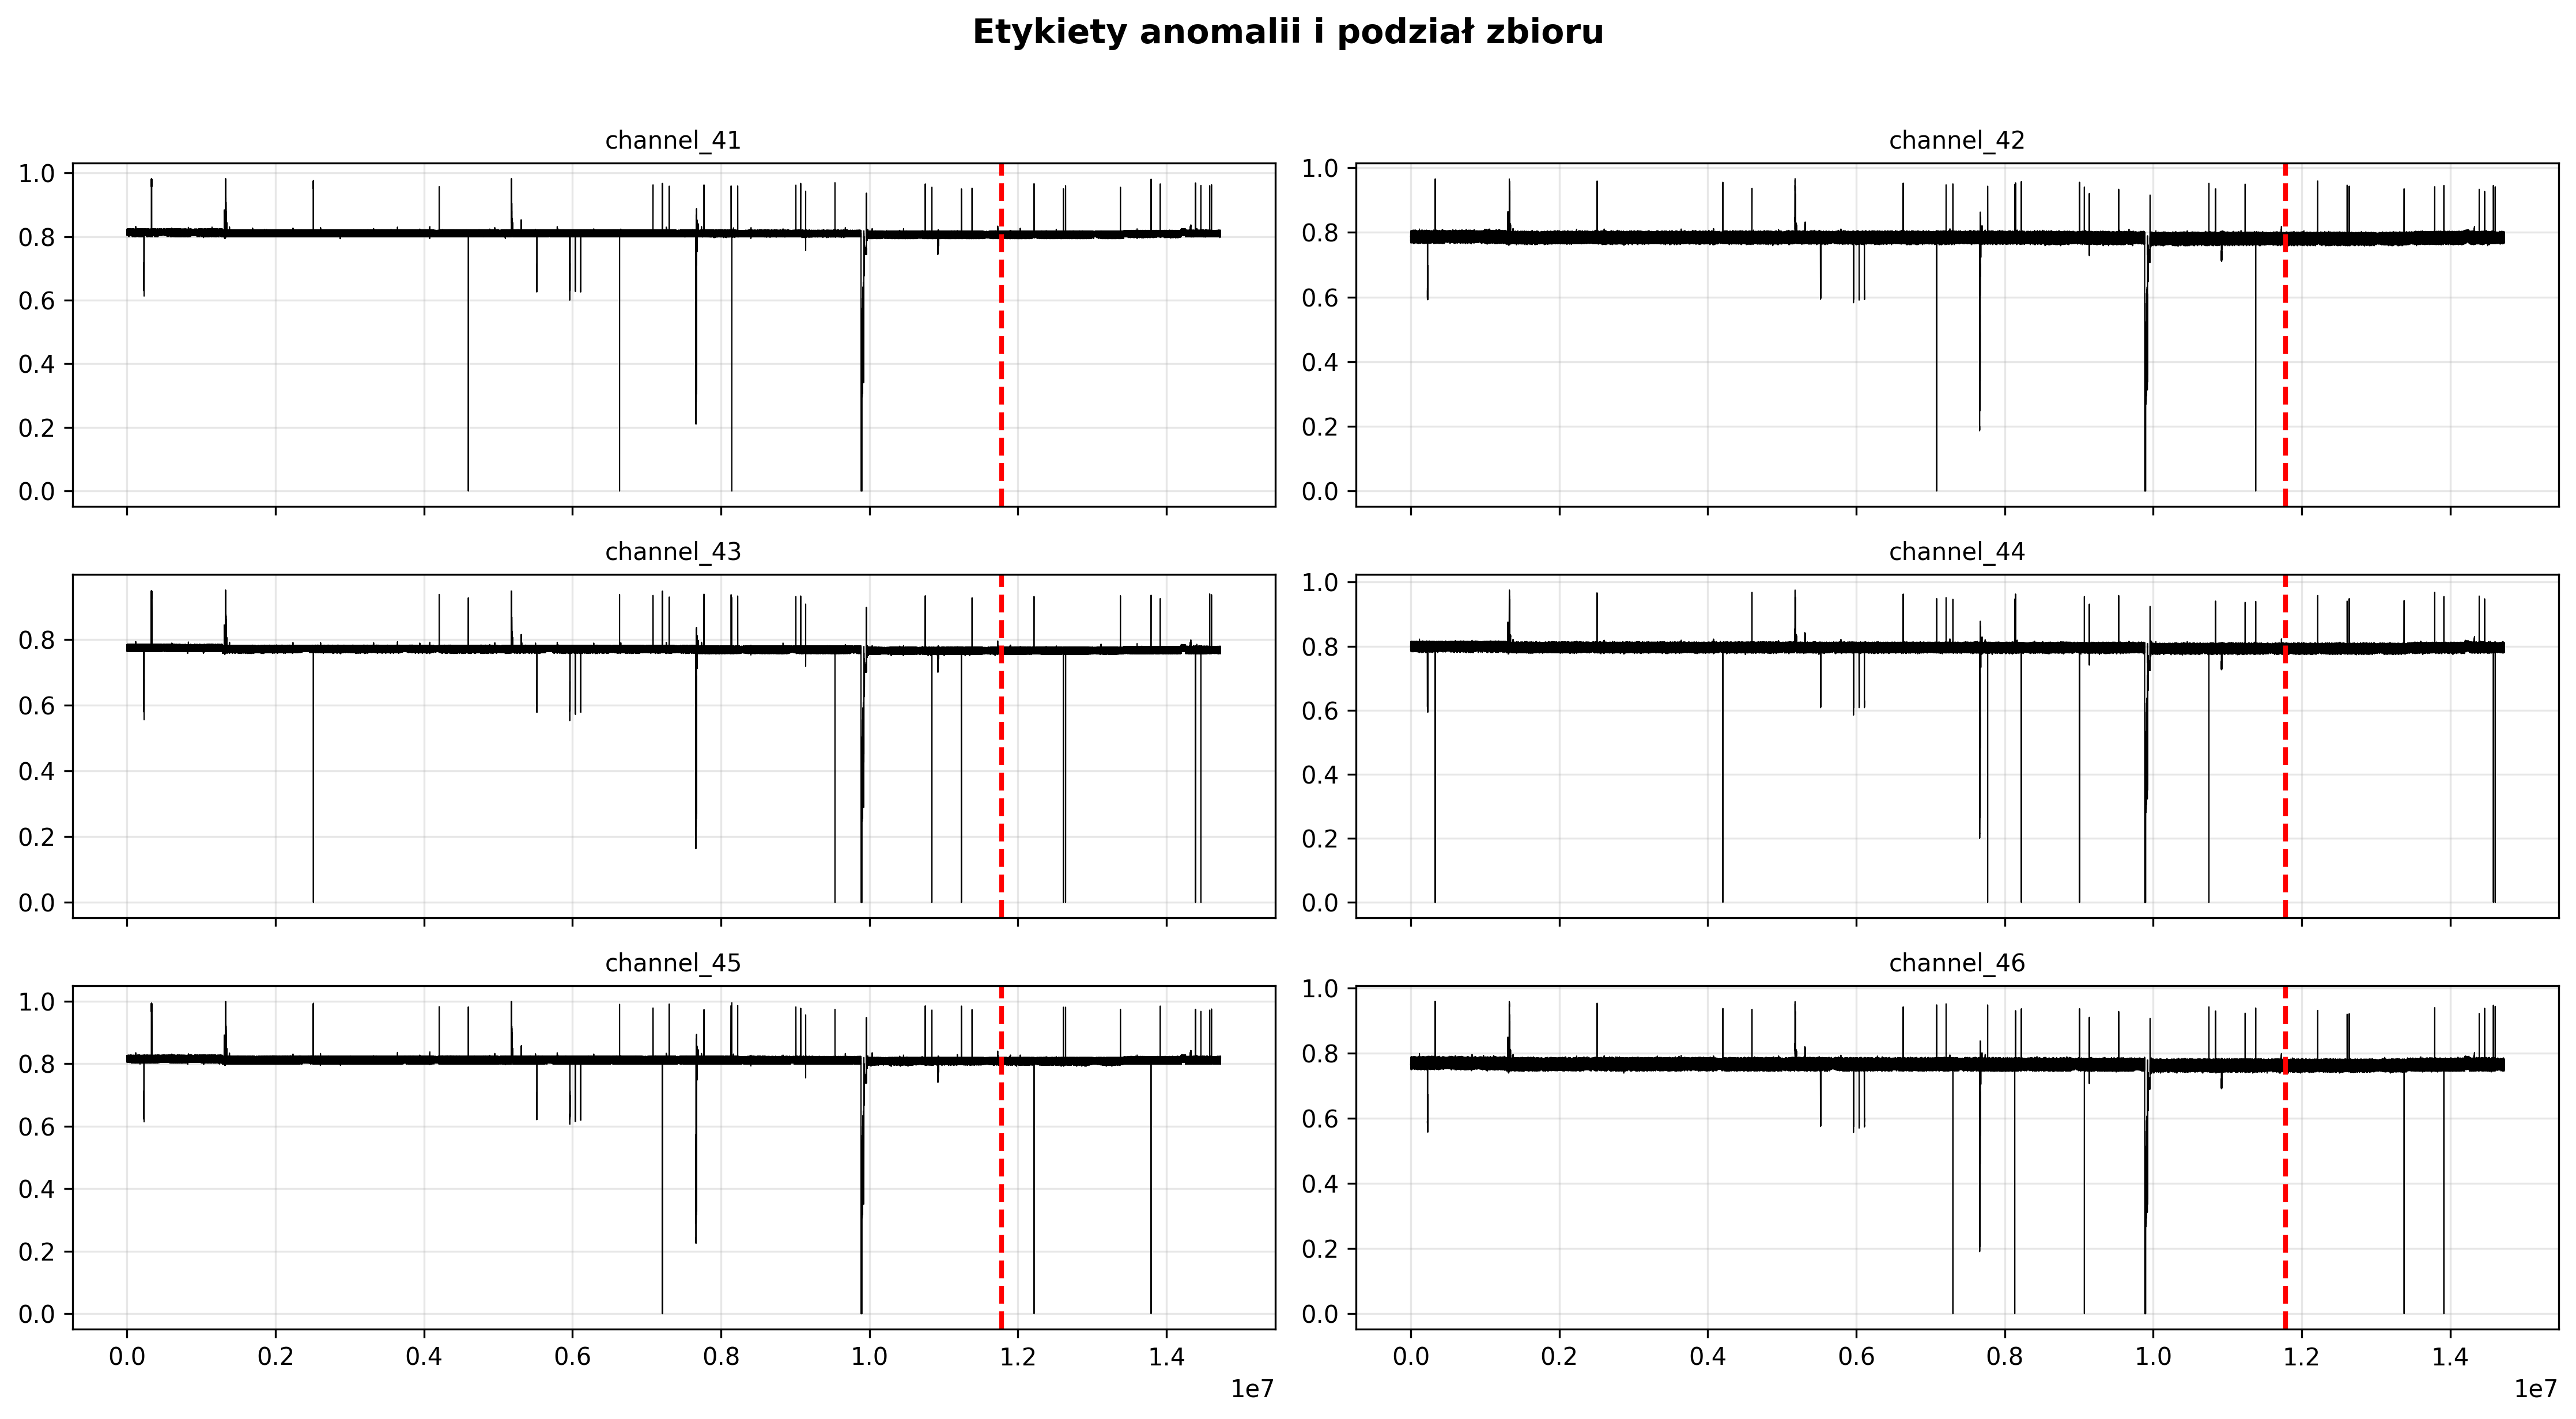
\includegraphics[width=0.9\textwidth]{fig_00_sig_overview.png}
		\caption{Przegląd sygnałów z podziałem chronologicznym 80/20.}
		\label{fig:00-sig-overview}
	\end{figure}
	Rysunek ~\ref{fig:00-sig-overview} przedstawia... umieszczony powyżej przedstawia przegląd rozkładu wartości danych we wszystkich badanych kanałach. Można zauważyć, że czerwona, przerywana linia oznacza linię podziału danych we wszystkich kanałach na zbiory uczące i testując
	\begin{figure}%[H]
		\centering
		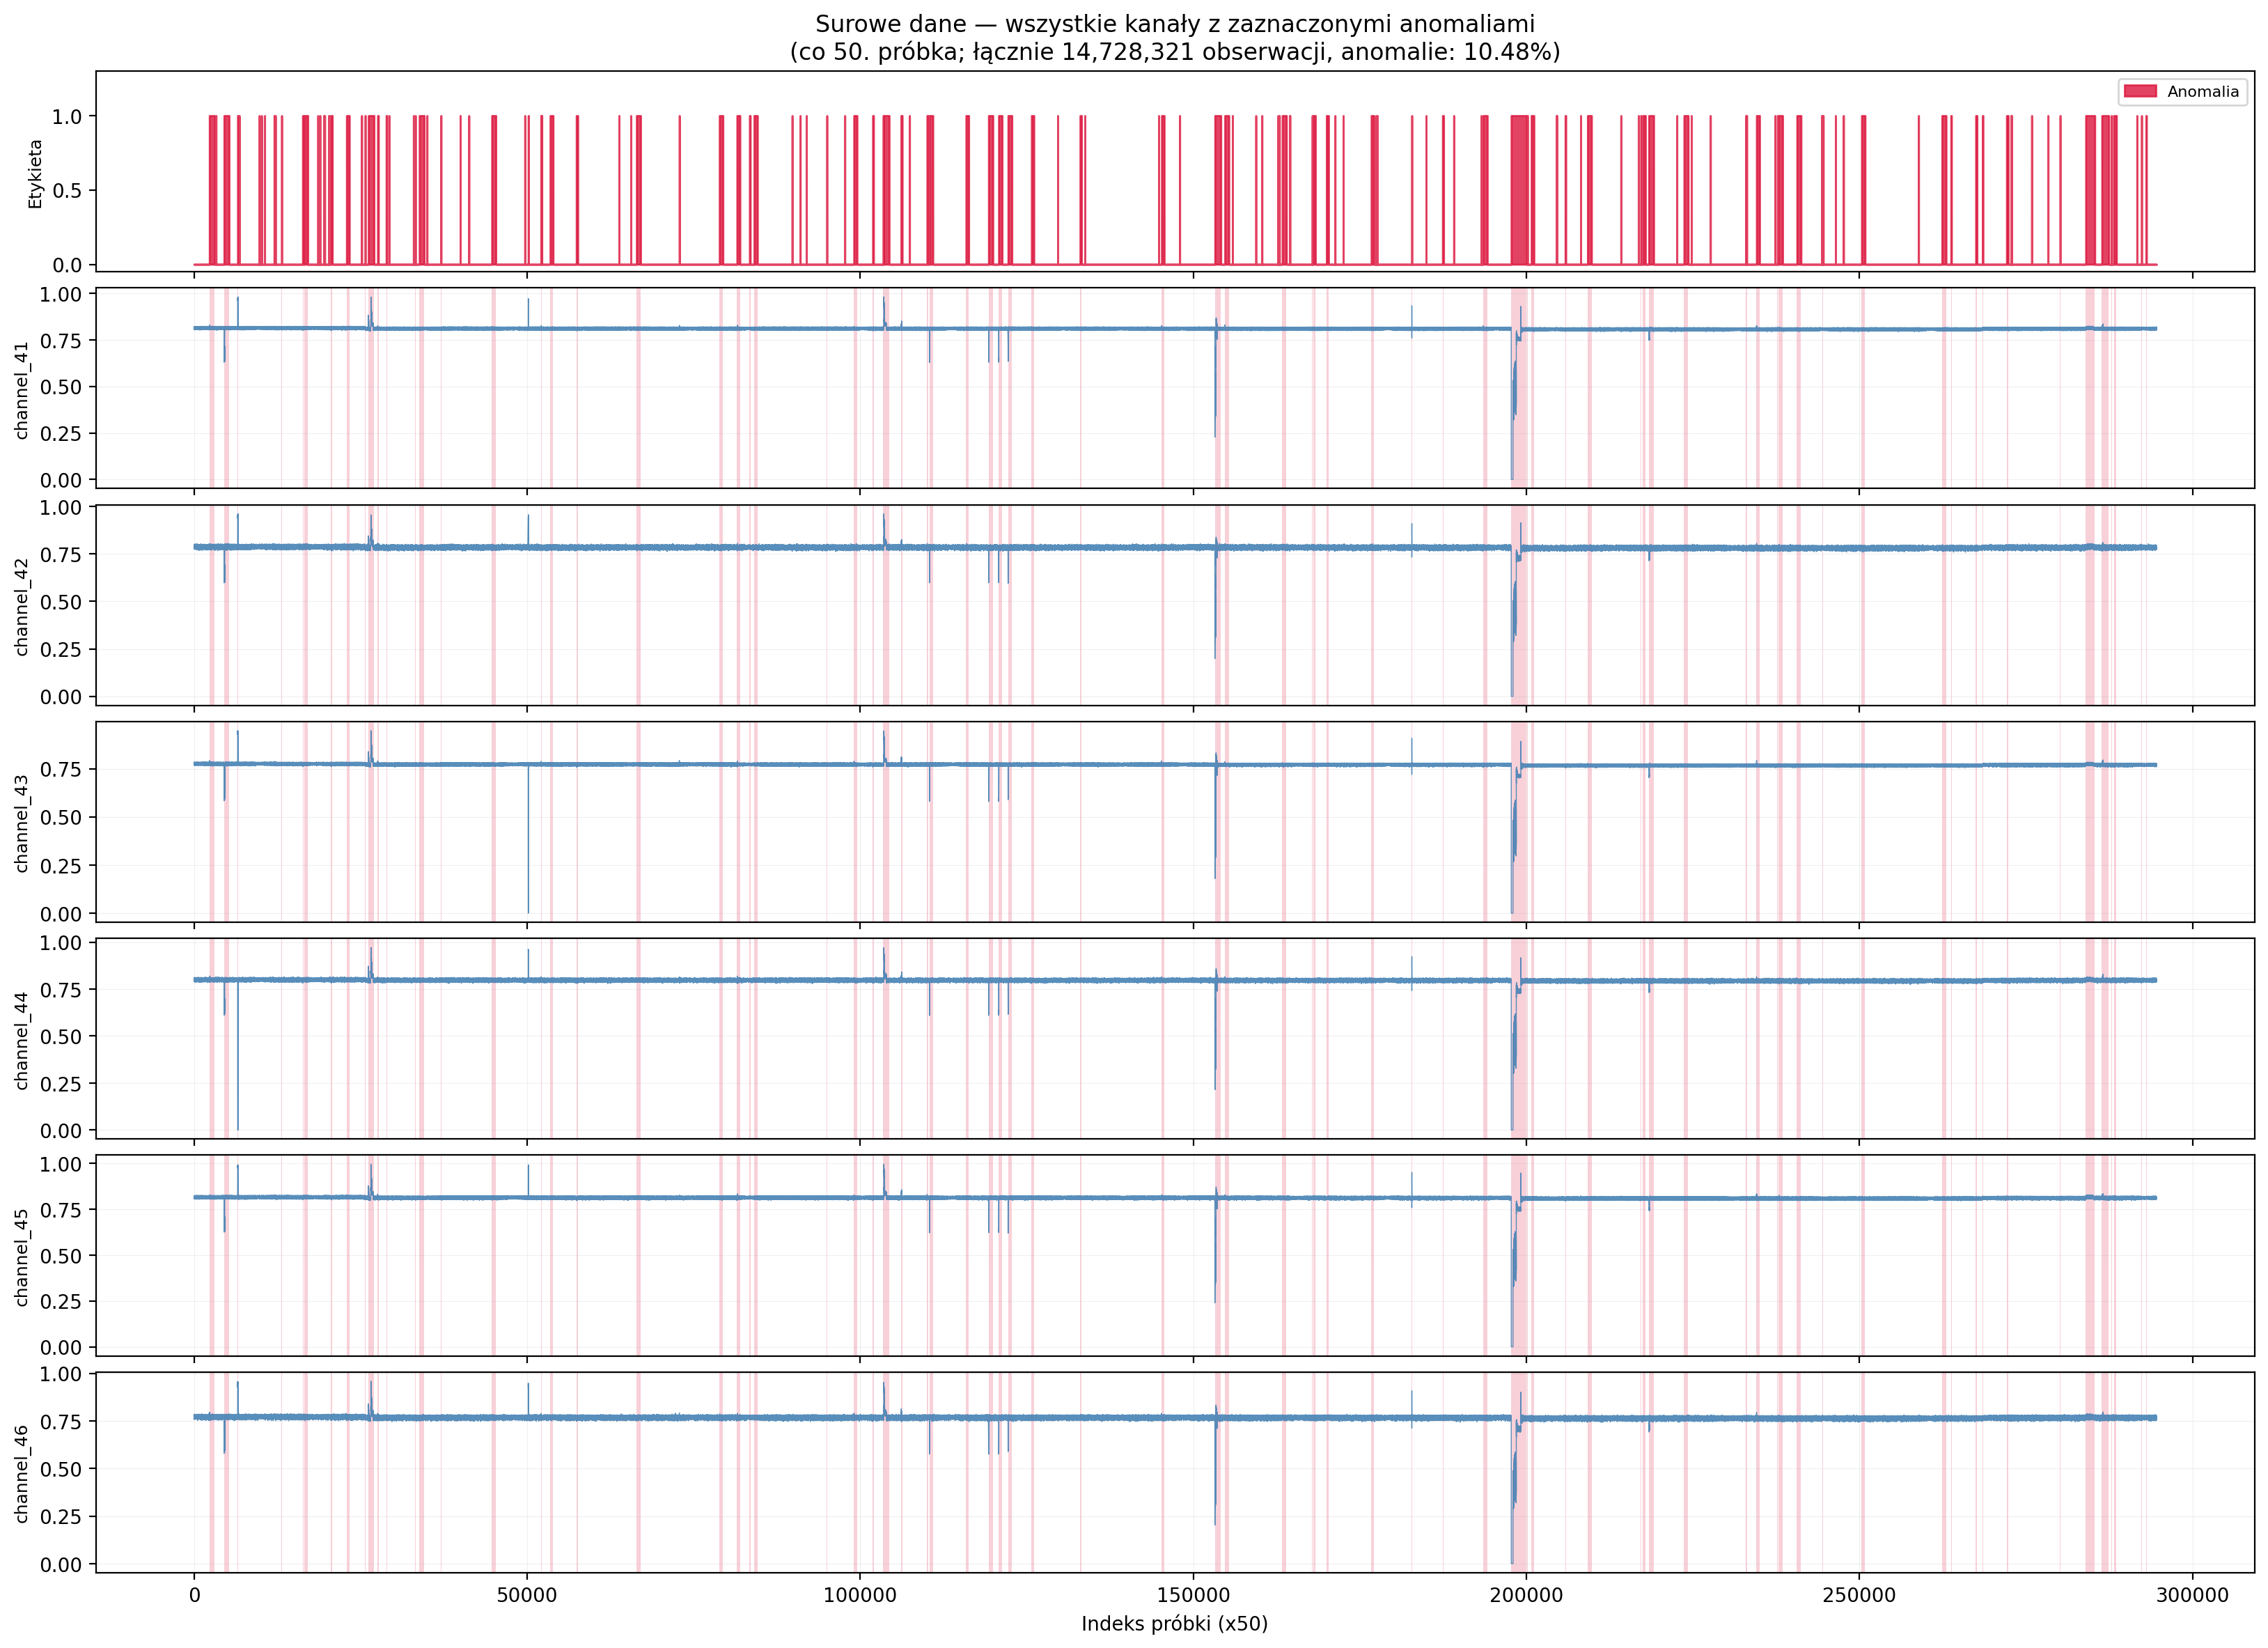
\includegraphics[width=0.9\textwidth]{fig_raw_01_overview.png}
		\caption{Wykres kanałów z występującymi anomaliami}
		\label{fig:raw:01-overview}
	\end{figure}
	
	\begin{figure}%[H]
		\centering
		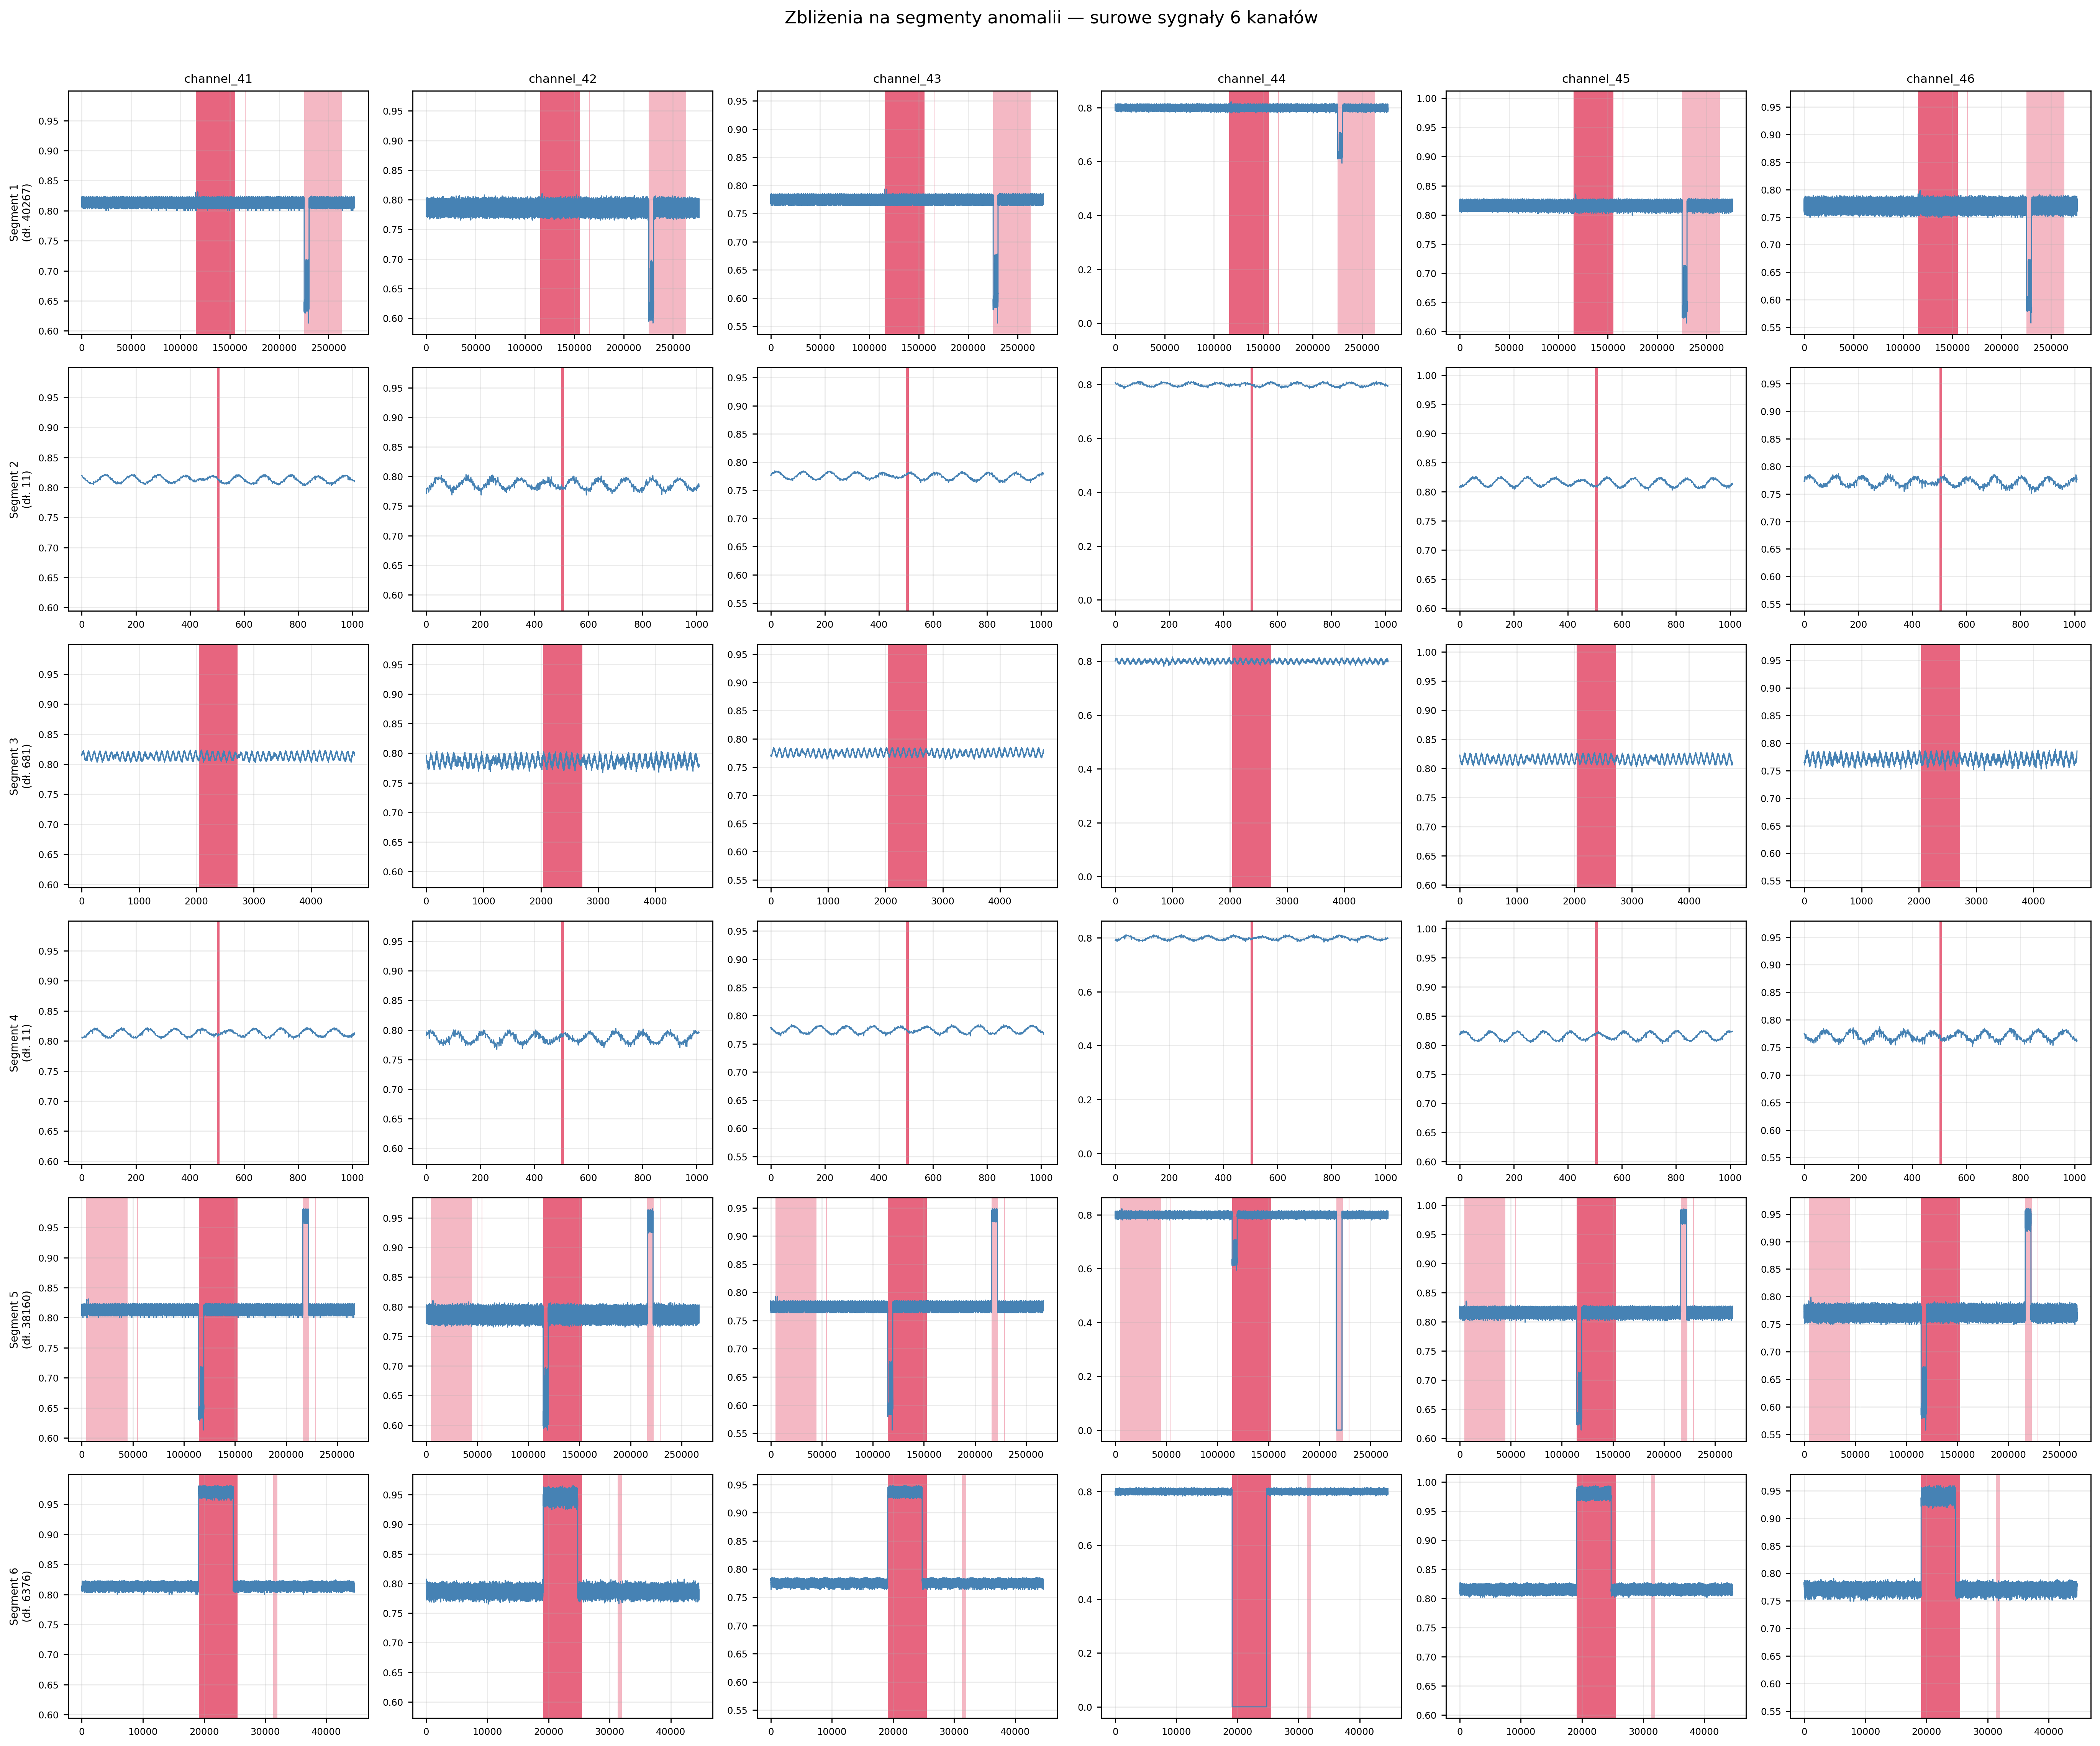
\includegraphics[width=0.9\textwidth]{fig_raw_02_zoom_segments.png}
		\caption{Przybliżone wykresy przedstawiające segmenty z anomaliami}
		\label{fig:raw:02-zoom-segments}
	\end{figure}
	
	Z kolei na rysunku ~\ref{fig:raw:01-overview} ukazano rozkład anomalii w zbiorze, aby pokazać, gdzie się skupiają. W celu ukazania skali pokazano tylko co pięćdziesiątą próbkę, aby pokazać skalę danych na których ewaluowano model. Aby jednak wskazać konkretniej jak wyglądają segmenty anomalii na tle danych normalnych zdecydowano dać przybliżenie na poszczególne segmenty, które zostały ukazane na rysunku ~\ref{fig:raw:02-zoom-segments}. Na obu tych rysunkach anomalie zostały oznaczone na czerwono, a intensywność barwy jest wprost proporcjonalna do gęstości tych danych na obszarze. 
	
	\subsection{Balans klas i rozkład anomalii}
	Na rysunku ~\ref{fig:00-class-balance} umieszczonym poniżej widać \comma\ jak rozłożenie danych na treningowe i testowe wpływa na odsetek anomalii. W analizowanej próbce, opartej na kanałach od 41 do 46 pierwsza część, czyli 11,7 mln danych zawiera 1,2 mln próbek oznaczonych jako anomalie, co przekłada się na 10,47 procent anomalii. W dalszych częściach badania ta część będzie służyć do uczenia modeli. Pozostała część zbioru, obejmująca pozostałą  część danych, posiada 310 tysięcy anomalii w sobie. Daje to łączenie 10,48 procent anomalii w całości. Oznacza to, że jest to wartość zdecydowanie większa niż w reszcie benchmarku, gdyż średnia danych całości wynosi ledwie 1,8 procent dla danych Mission-1\cite{kotowski2024esaadb}, co czyni badaną część skrajnie niezbilansowaną, co może mieć wpływ na końcowy wynik.
	\begin{figure}%[H]
		\centering
		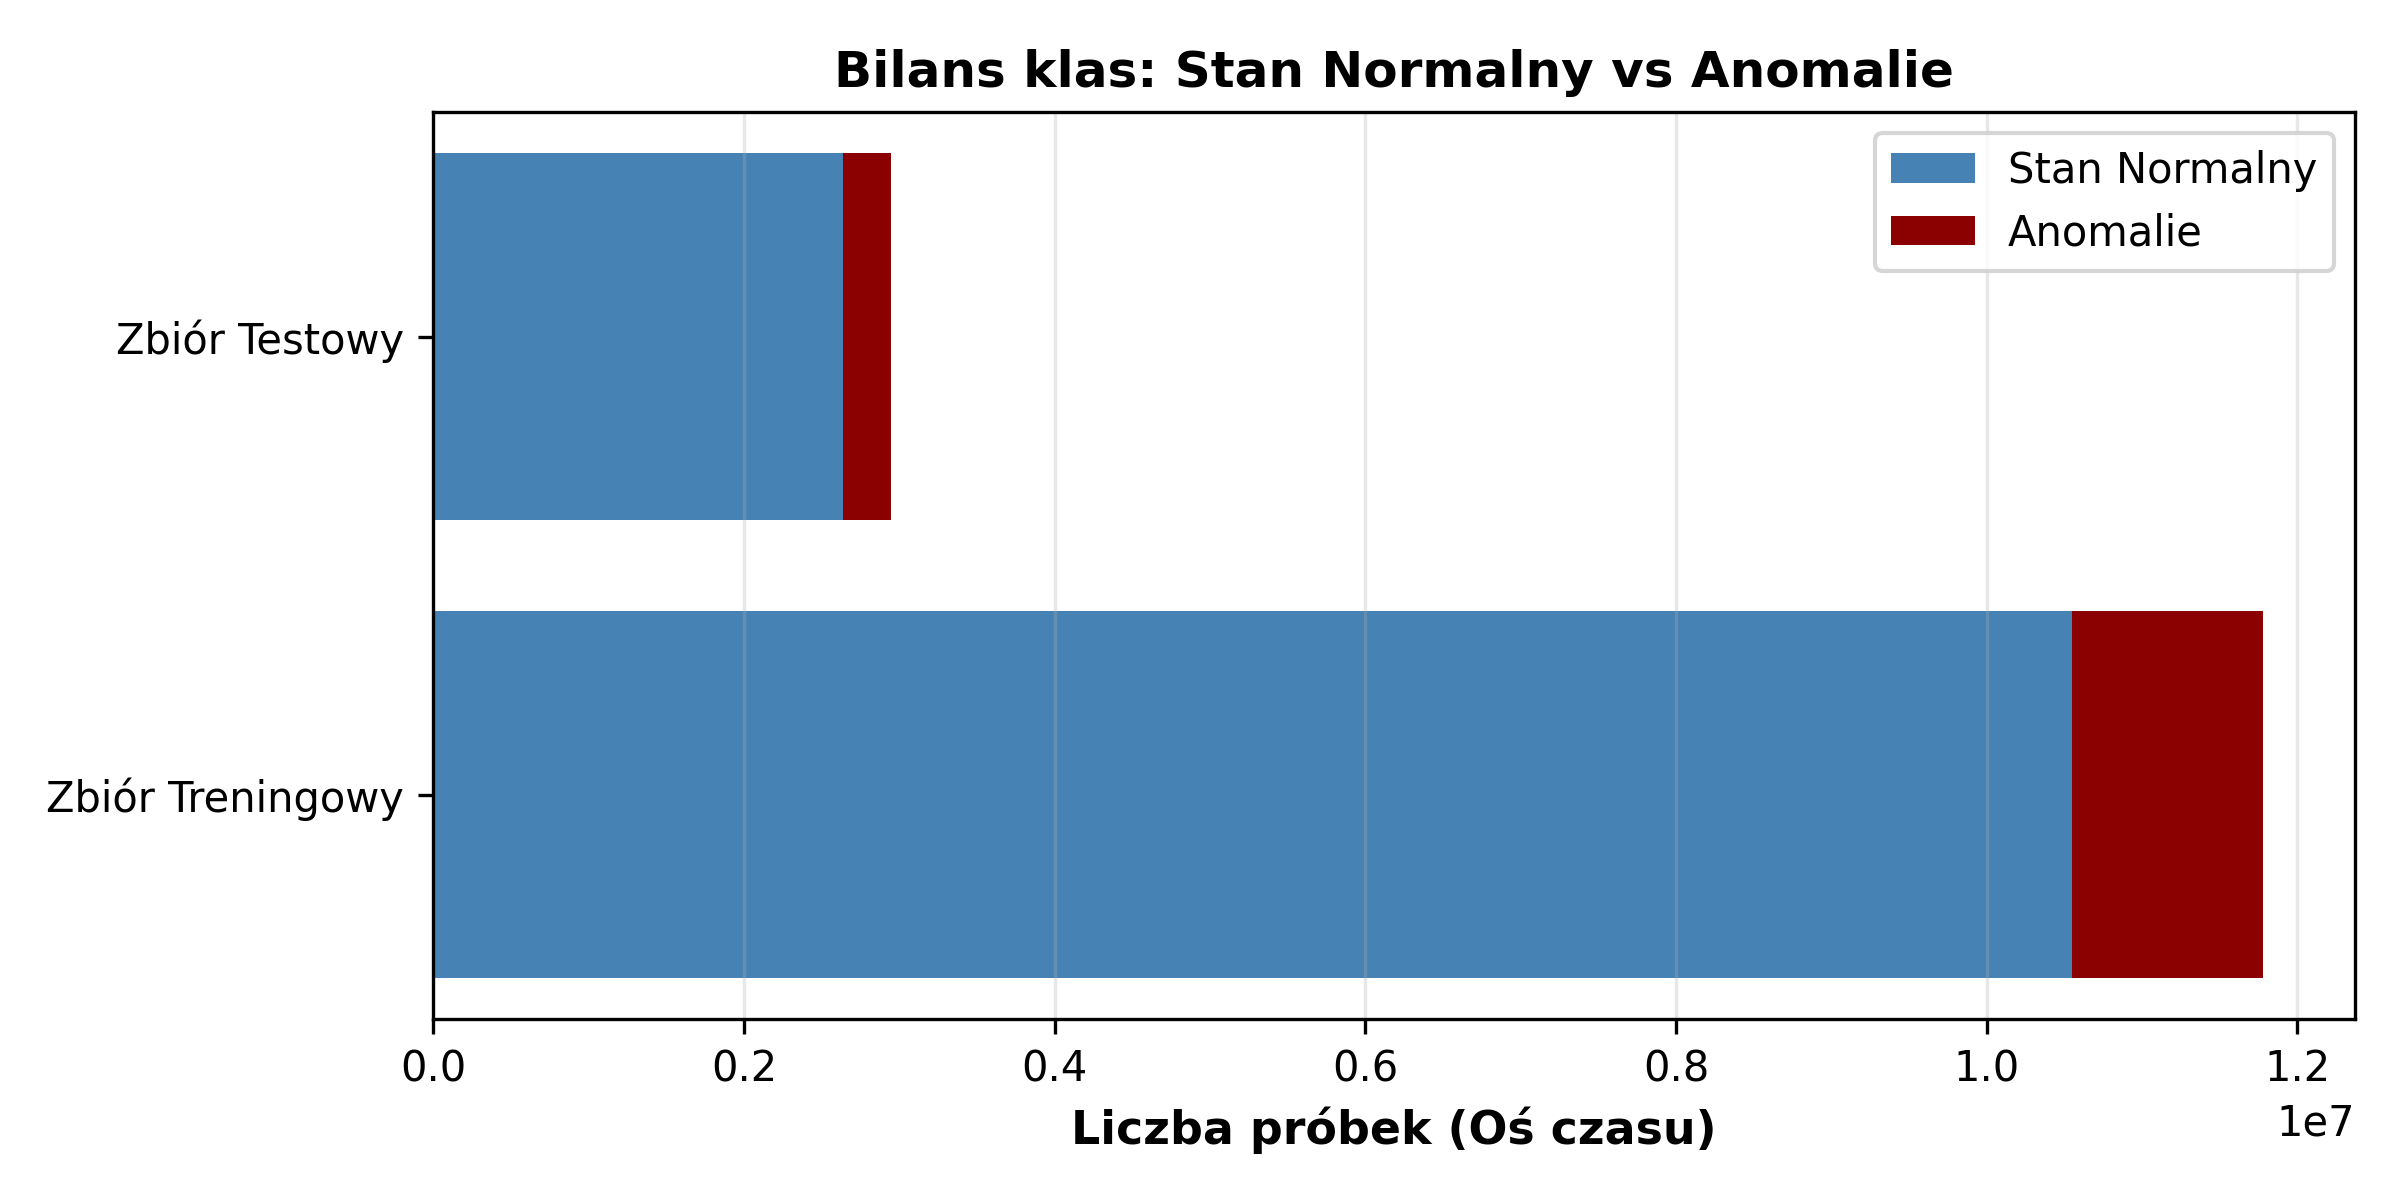
\includegraphics[width=0.9\textwidth]{fig_00_class_balance.png}
		\caption{Bilans klas oraz rozkład występowania anomalii w zbiorach danych.}
		\label{fig:00-class-balance}
	\end{figure}
	Na poniższym rysunku ~\ref{fig:00-anomaly-dist} widać z kolei jak anomalie rozkładają się w poszczególnych zbiorach. Z kolei rysunek ~\ref{fig:raw:03-distributions} przedstawia rozkład wartości surowych dla wszystkich 6 analizowanych kanałów, z wyróżnionym rozróżnieniem na dane normalne i anomalie, w formie histogramu, jakie wartości najczęściej były klasyfikowane. 
	\begin{figure}%[H]
		\centering
		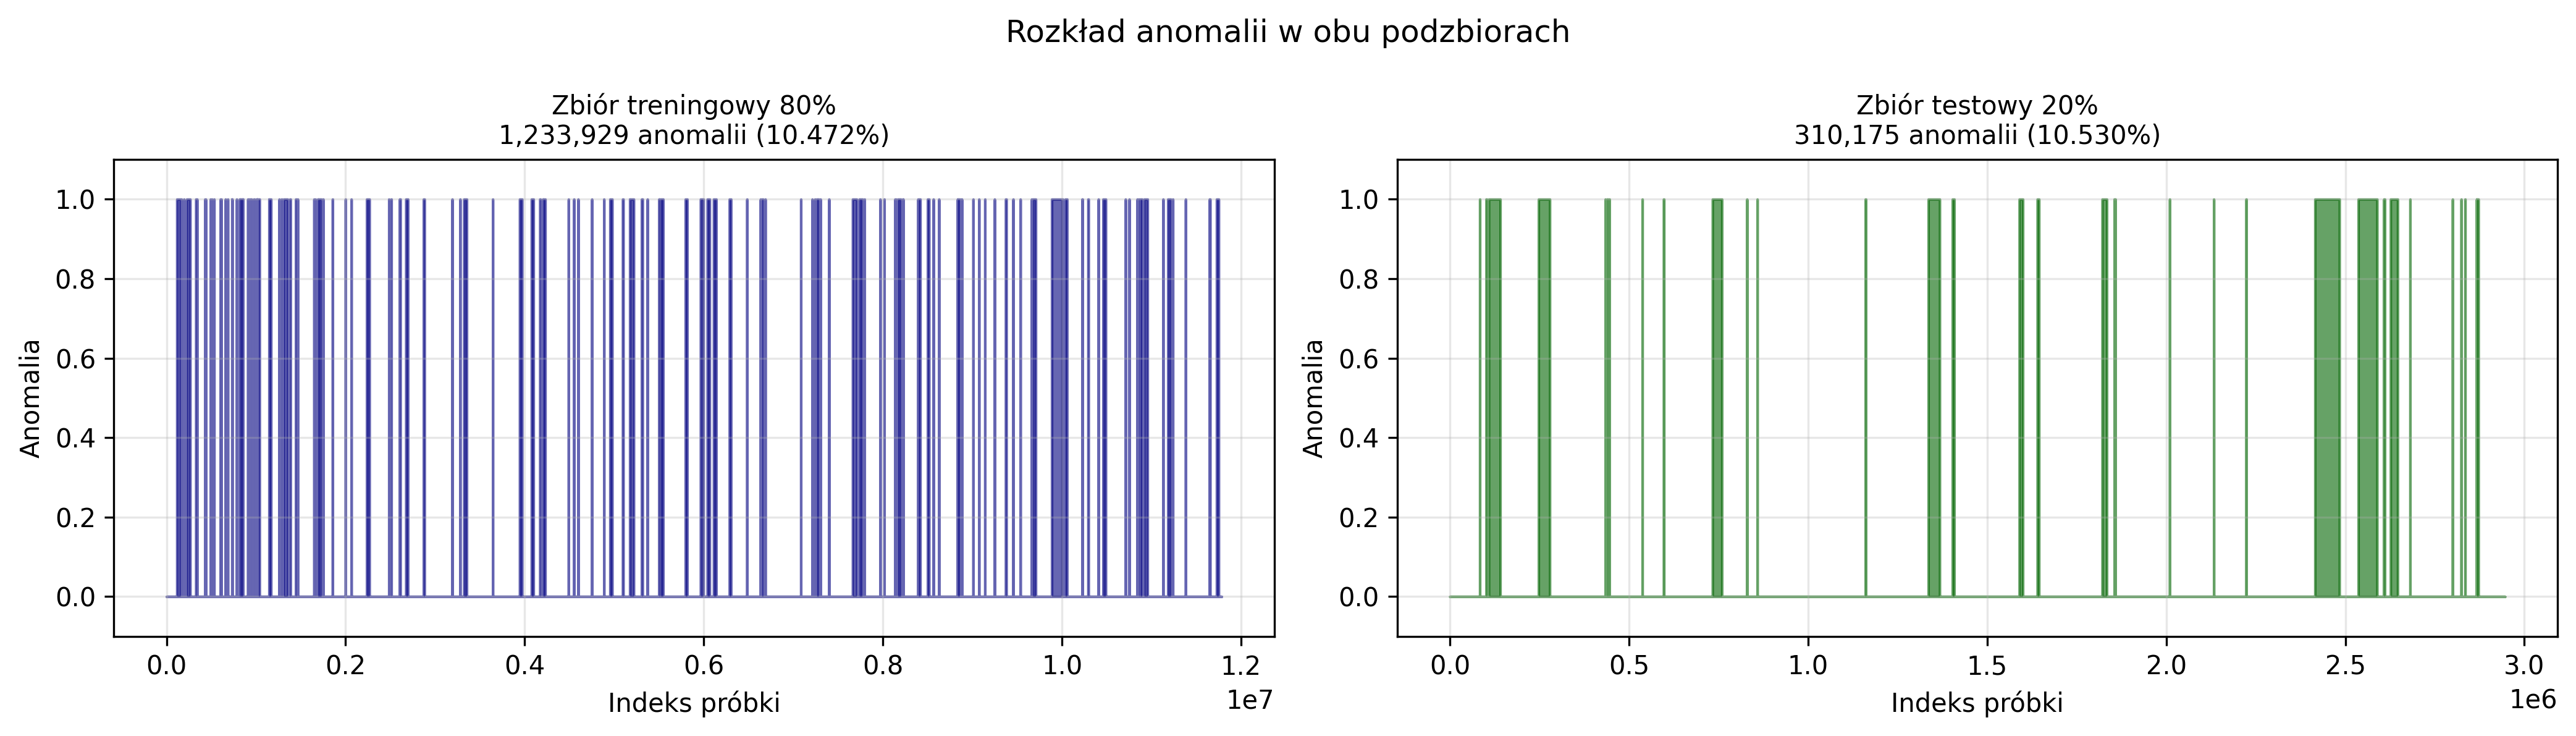
\includegraphics[width=0.9\textwidth]{fig_00_anomaly_dist.png}
		\caption{Rozkład anomalii w zbiorach treningowym i testowym}
		\label{fig:00-anomaly-dist}
	\end{figure}
	
	\begin{figure}%[H]
		\centering
		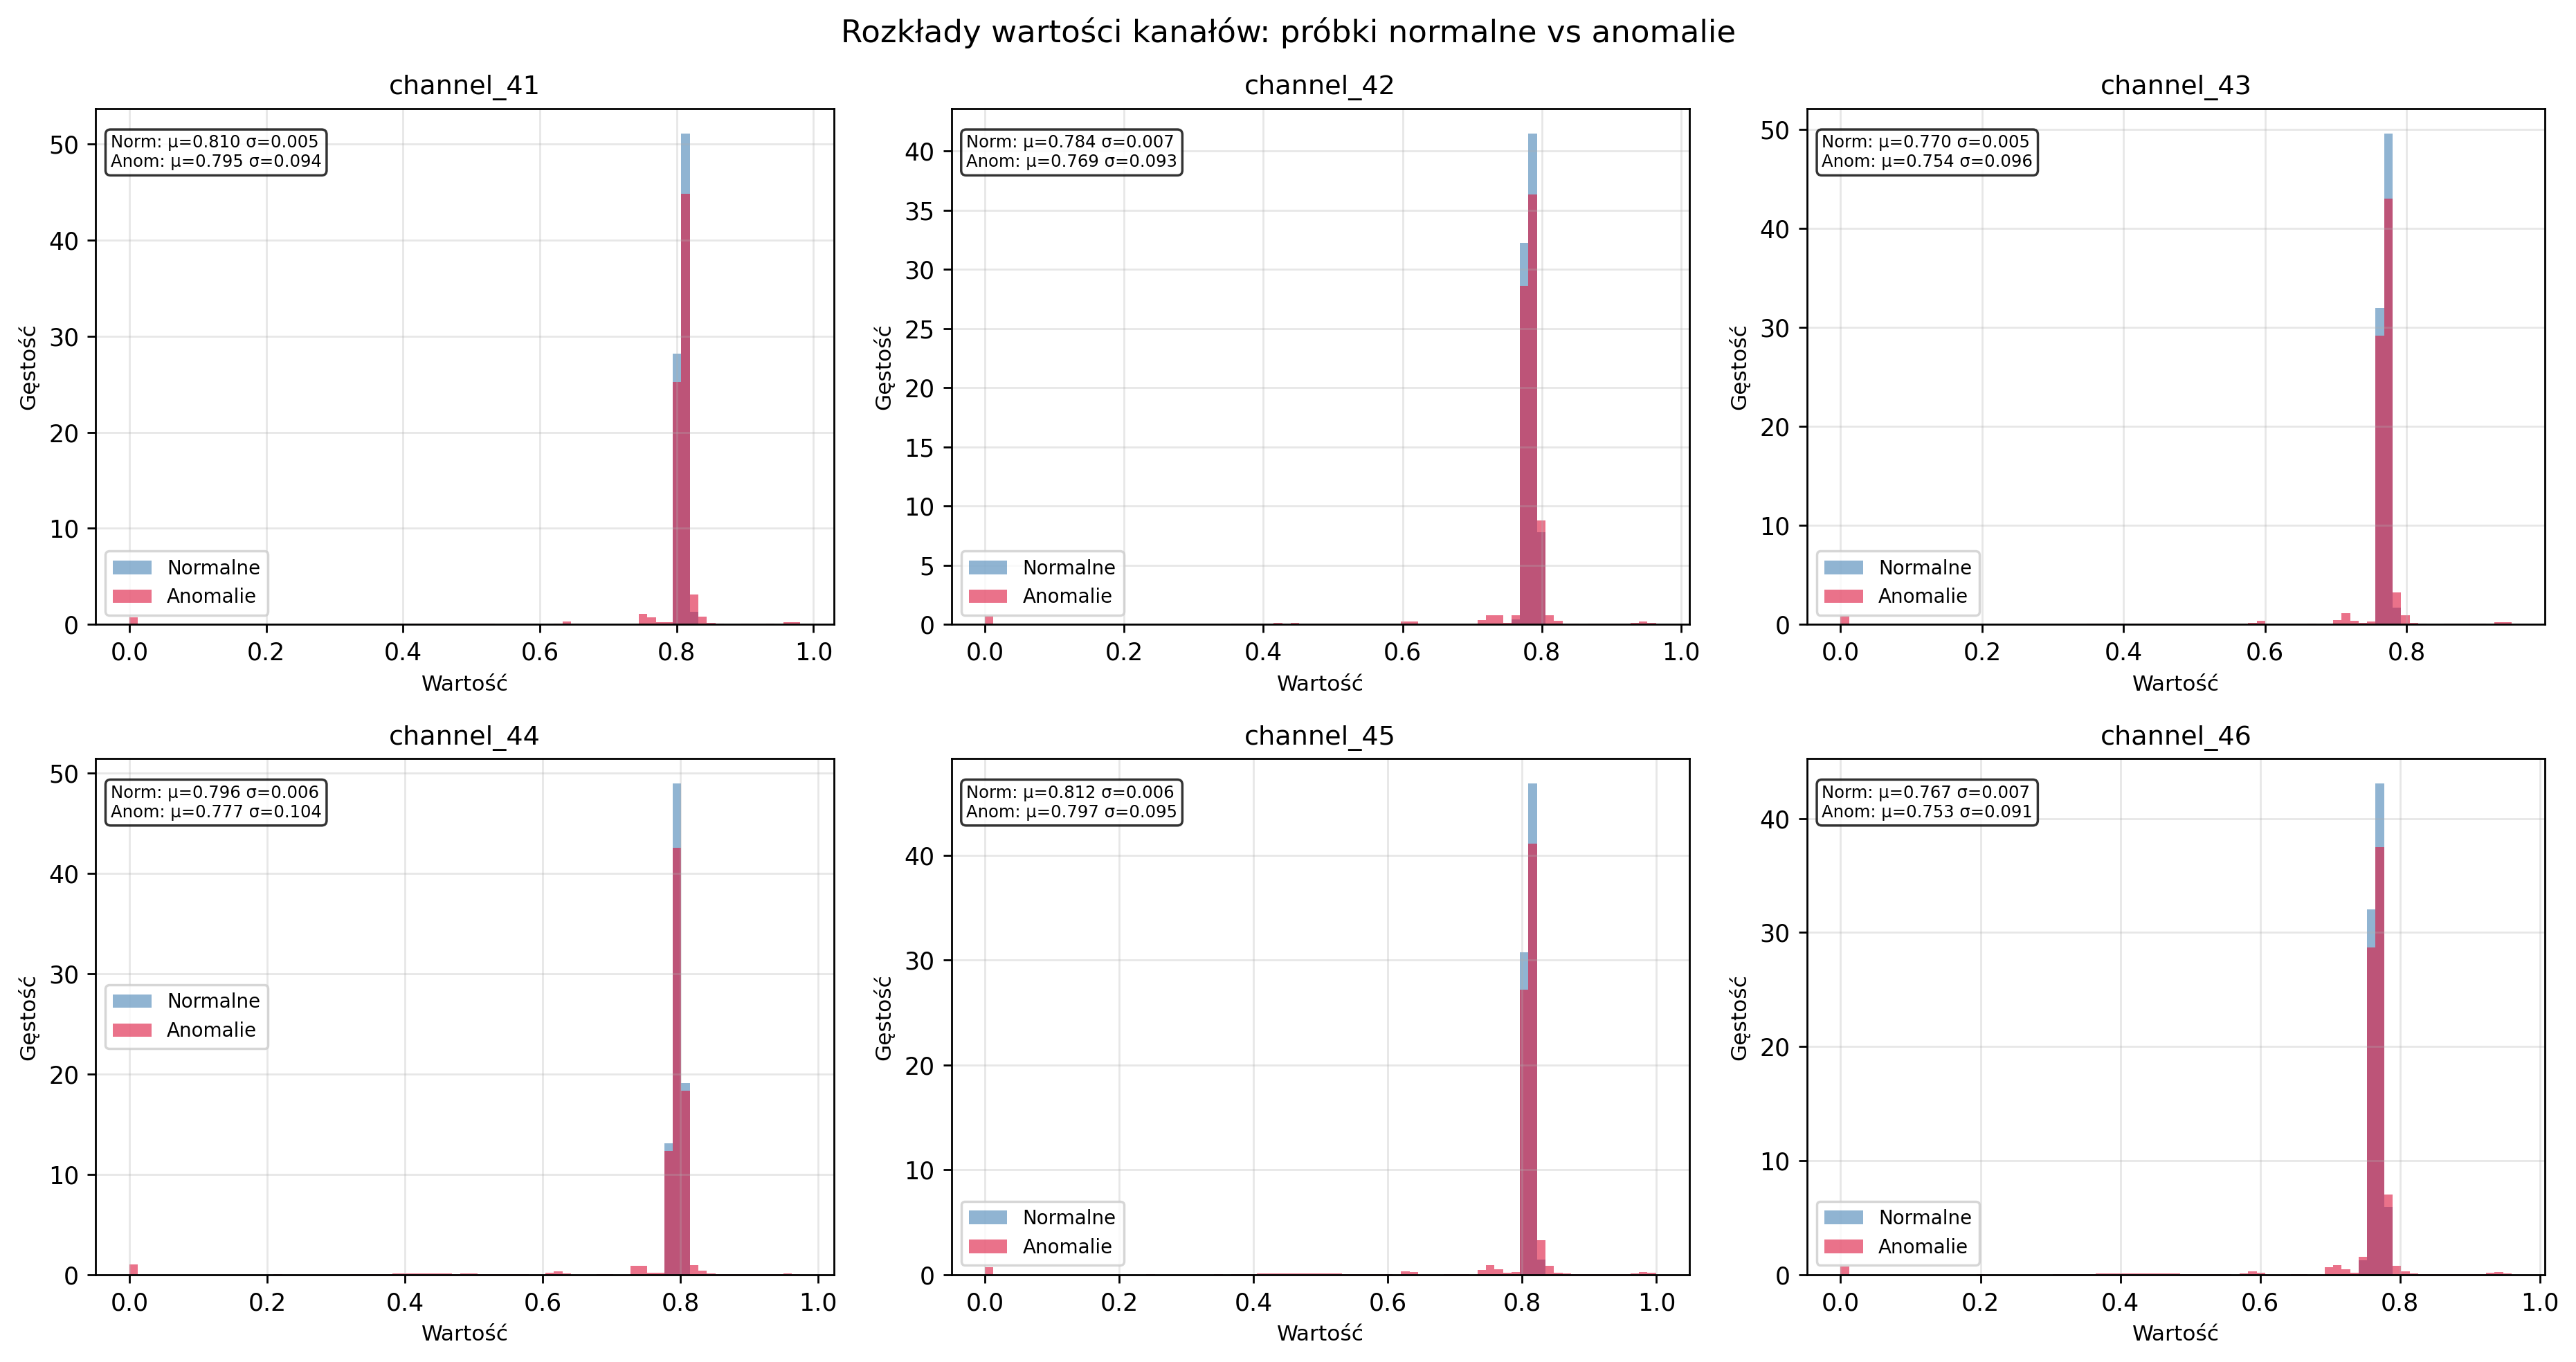
\includegraphics[width=0.9\textwidth]{fig_raw_03_distributions.png}
		\caption{Rozkład wartości kanałów}
		\label{fig:raw:03-distributions}
	\end{figure}
	
	
	
	\section{Środowisko i implementacja}
	Do przeprowadzenia badań wykorzystano laptop posiadający procesor AMD Ryzen 5 5600H, posiadający 6 rdzeni i 12 wątków, 16 GB pamięci RAM i zintegrowaną kartę graficzną AMD Radeon™ Graphics z systemem operacyjnym Windows 11. Wszystkie programy zostały wykonane w języku Python w wersji 3.12.2 z wykorzystaniem  poniższych wersji bibliotek:
	\begin{table}%[H]
		\centering
		\caption{Wersje najważniejszych bibliotek wykorzystanych w eksperymentach}
		\label{tab:biblioteki}
		\begin{tabular}{ll}
			\hline
			\textbf{Biblioteka} & \textbf{Wersja} \\
			\hline
			Keras & 3.13.0 \\
			Matplotlib & 3.10.8 \\
			NumPy & 1.26.4 \\
			Pandas & 2.3.3 \\
			Scikit-learn & 1.8.0 \\
			TensorFlow & 2.20.0 \\
			TensorFlow Intel & 2.17.0 \\
			TensorFlow IO GCS Filesystem & 0.31.0 \\
			\hline
		\end{tabular}
	\end{table}
	
	Programy zostały wykonane w środowisku Visual Studio Code. W domyślnym folderze ze strukturą projektu znajdują się wszystkie kody spełniające poszczególne funkcje, takie jak przygotowanie danych, inżynieria cech, testowanie wszystkich trzech klas metod i porównanie wszystkich metod pod względem czasu potrzebnego do wykonania poszczególnej iteracji algorytmu z jednym zestawem parametrów, a także zużycia pamięci dla każdej z nich. Każdy program swoje wyniki w osobnym podfolderze folderu „results”. 
	
	
	\section{Preprocessing i inżynieria cech}
	Przed rozpoczęciem właściwych prac dokonano przygotowania danych do testowania. Dane w momencie publikacji już były uprzednio znormalizowane do przedziału $[0, 1]$ \cite{kotowski2024esaadb}. Dokonano tego zgodnie z polityką prywatności Europejskiej Agencji Kosmicznej w celu uniknięcia przypadkowego ujawnienia wrażliwych danych specyficznych dla misji. Z racji działania na danych chronologicznych, w ramach wzięcia pod uwagę lokalnego kontekstu czasowego, zastosowano technikę okna kroczącego. Polega ona na tym, że dla każdej próbki analizie poddano zarówno bieżącą wartość, jak i ustaloną wartość poprzednich danych. Okno długości $w$, w chwili $t$ obejmuje próbki od $t - w +1$ do $t$.  Używając wartości w tym oknie obliczono trzy cechy opisujące lokalne zachowanie sygnału
	
	Pierwszą z nich było odchylenie od lokalnego poziomu bazowego, określa ono jak bardzo wartość bieżąca różniła się od średniego poziomu obserwowanego w szerokości okna kroczącego. Pozwala ono na znalezienie momentu, w którym namierzono sytuację odchylenia sygnału od typowego przebiegu, co może sugerować występowanie anomalii. 
	\begin{align}
		d_t &= x_t - \mu_t^{(w)}, \label{eq:dt} \\
		\mu_t^{(w)}   &= \frac{1}{w} \sum_{i=t-w+1}^{t} x_i. \label{eq:mu}
	\end{align}
	gdzie $d_t$ oznacza wyznaczone odchylenie w chwili czasu $t$, a $ \mu_t^{(w)}$ jest lokalną średnią arytmetyczną z okna o rozmiarze $w$
	
	Drugą z nich jest odchylenie standardowe wartości znajdujących się w oknie kroczącym. Im większe okno, tym szerszy zakres. Opisuje lokalną zmianę sygnału. Cecha ta pozwala na znalezienie fragmentu, w którym sygnał stał się nagle niestabilny, lub segmentu z większym rozrzutem danych.
	
	\begin{equation}
		\sigma_t^{(w)} =
		\sqrt{
			\frac{1}{w}
			\sum_{i=t-w+1}^{t}
			\left(x_i - \mu_t^{(w)}\right)^2
		}.
	\end{equation}
	gdzie $\sigma_t^{(w)}$ jest wyliczonym lokalnie odchyleniem standardowym.
	
	Ostatnią z wartości, którą wyznaczono z pomocą okna kroczącego jest tempo zmiany sygnału pomiędzy próbkami. Pomaga ono namierzyć moment, w którym sygnał gwałtownie zmienia swój charakter. Zależnie od wyniku, może być to skok w górę lub gwałtowny spadek. W ramach badania za tempo zmiany uznano różnicę w charakterze wartości względem pięciu ostatnich próbek. Jest to wartość, którą empirycznie dobrano we wstępnej fazie eksperymentów, gdyż obliczanie różnicy dla sąsiadujących próbek ($x_t - x_{t-1}$) nadmiernie wzmacniało szum czujników. Wartość 5 pozwala zachować dynamikę sygnału, jednocześnie wygładzając szum. Wartość tę wyznacza wzór: 
	\begin{equation}
		r_t^c = x_t^c - x_{t-5}^c
	\end{equation},
	gdzie $c$ oznacza indeks kanału telemetrycznego, a $r_t^c$ reprezentuje tempo zmiany sygnału (ang. \english{rate of change}) dla kanału w chwili $t$.
	
	
	
	Wszystkie te cechy mogą tworzyć prostą reprezentację przebiegu sygnału. Po przetworzeniu danych przez okno kroczące każdy z kanałów został opisany dodatkowymi, lokalnymi cechami, a dane wejściowe dla modeli dostały rozszerzoną reprezentację i charakterystykę sygnału. Natomiast to rozwiązanie posiada jeden problem. Dla pierwszych próbek nie można obliczyć cech z pomocą okna kroczącego, bo brakuje wcześniejszych danych tworzących kontekst, który stanowi punkt odniesienia do wyliczania metryk. Proporcjonalnie, im większe okno, tym więcej danych utracono, gdyż wcześniejsze wiersze usunięto. Dzięki temu, każda próbka posiadała pełny zestaw cech. Pomimo tego, że autorzy zbioru dokonali wstępnej normalizacji \cite{kotowski2024esaadb}, obliczone cechy lokalne za pomocą techniki okna kroczącego zostały poddane dodatkowej standaryzacji z-score za pomocą funkcji \texttt{StandardScaler}. Parametry zostały wyliczone w ten sposób, czyli odchylenie standardowe i średnia tylko dla danych normalnych zbioru treningowego, co zapobiega przedostaniu się anomalii do modelu.
	
	\section{Dobór okna kroczącego}
	W ramach doboru rozmiaru okna kroczącego przeprowadzono eksperyment testujący wyniki głównych miar w zależności od rozmiaru okna kroczącego, a co za tym idzie cech z nim związanych. Do badań użyto 38 rozmiarów, od pojedynczych jedności, a konkretnie 5, przez dziesiątki, setki, a kończąc na 150 tysiącach jednostek. Natomiast w ramach pierwszej próby użyto tylko okna rozmiarów do ewaluacji od 5 do 5000, aby dać umiarkowane pojęcie o charakterze, wraz z wynikami, w celu znalezienia maksimum, odpowiednio zwiększano granice, aż zwiększanie rozmiarów okien nie dawało poprawy wyników. Do testów użyto algorytmu IQR wraz z wartością mnożnika równą 0.5. Wyniki tego badania pokazuje rysunek ~\ref{fig:01b-large-windows} zamieszczony poniżej.
	\begin{figure}%[H]
		\centering
		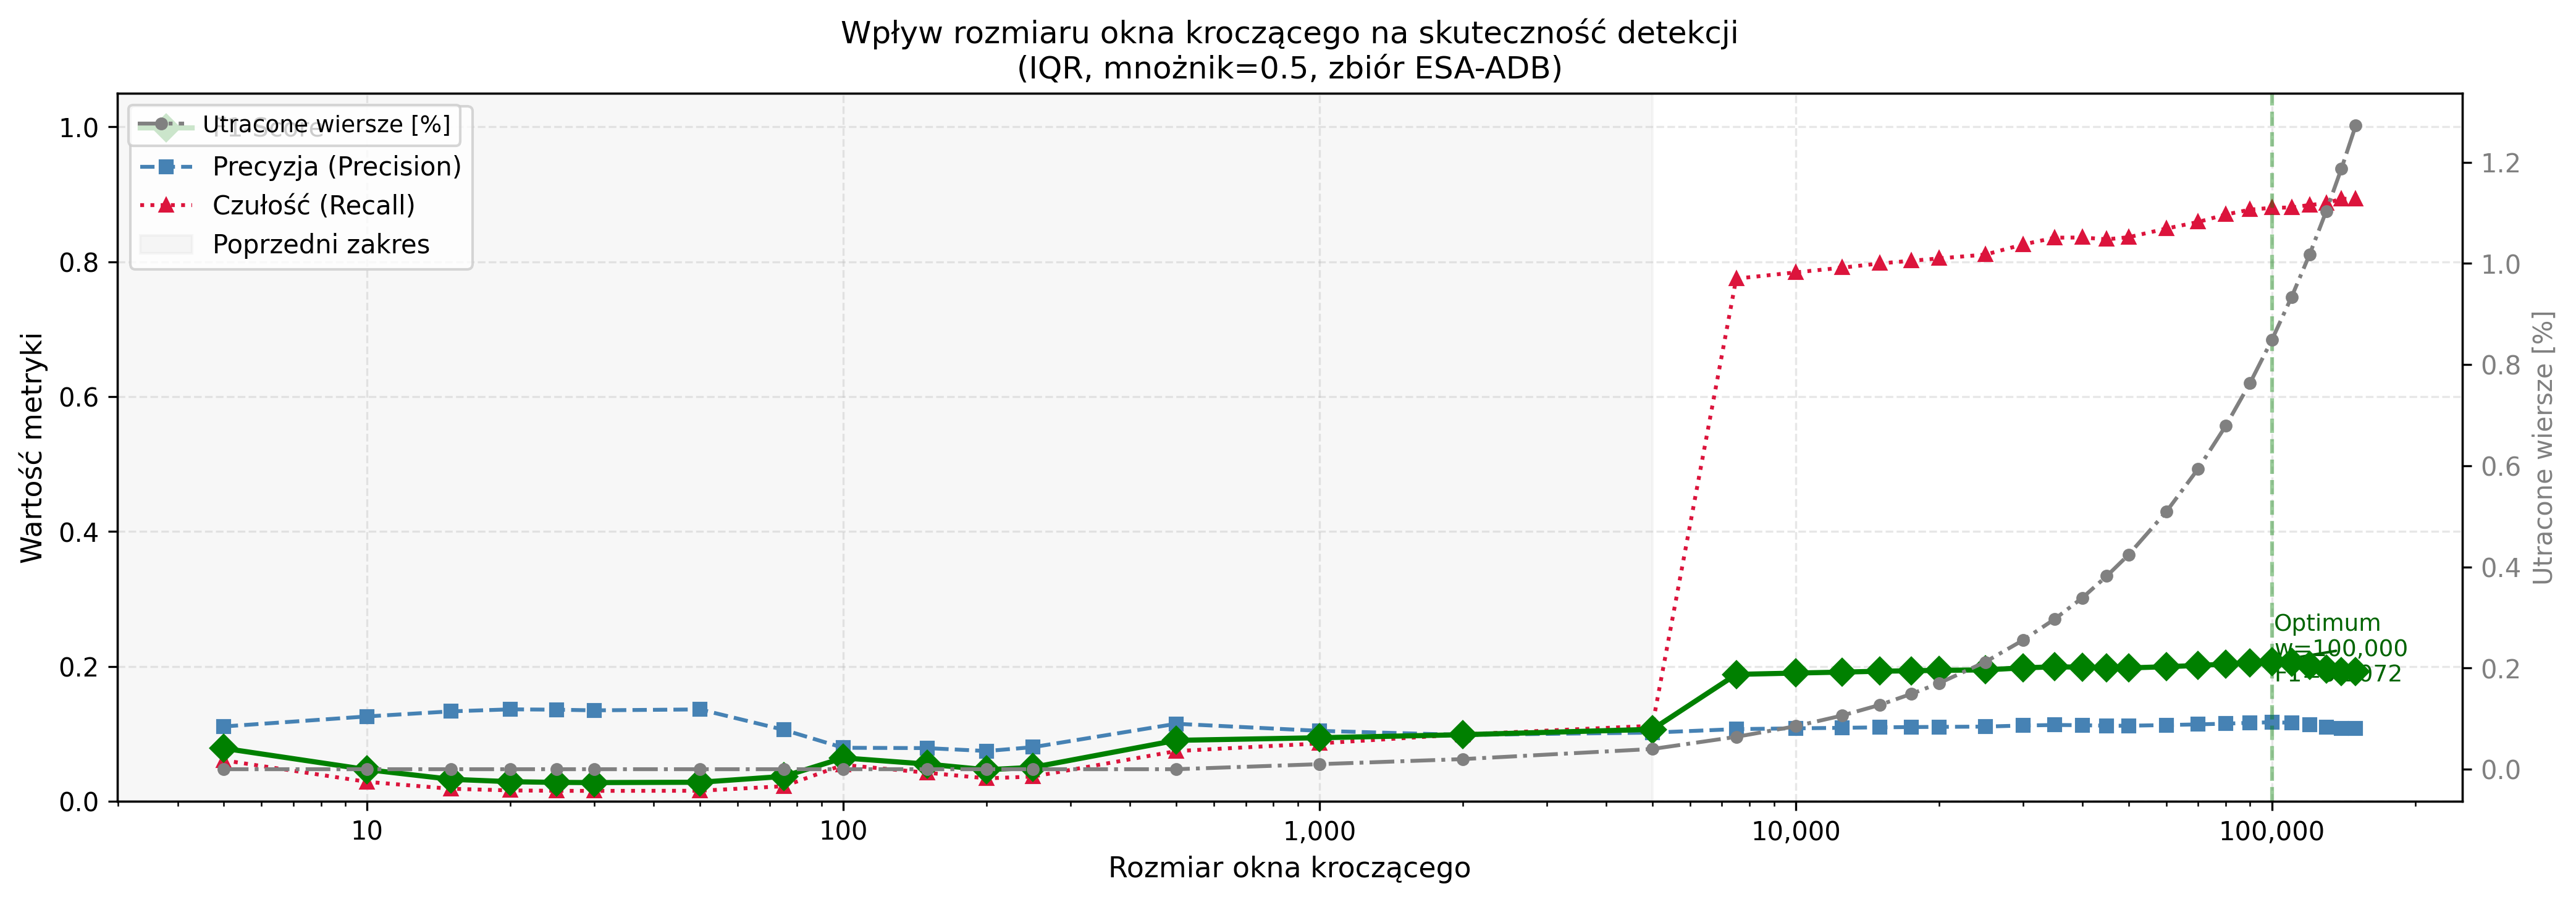
\includegraphics[width=0.9\textwidth]{fig_01b_large_windows.png}
		\caption{Analiza wpływu rozmiaru okna kroczącego na jakość detekcji anomalii.}
		\label{fig:01b-large-windows}
	\end{figure}
	
	
	
	\begin{figure}%[H]
		\centering
		
\includegraphics[width=0.9\textwidth]{fig_02b_heatmap.png}
		\caption{Macierz korelacji i wpływu dobieranych parametrów na skuteczność modelu.}
		\label{fig:02-heatmap}
	\end{figure}
	
	Dla początkowych wartości okna wyniki prezentują się mało interesująco, stopniowy wzrost parametru precyzji, do wartości 50, gdzie wartość wyniosła 0.1364, lecz po tym jesteśmy świadkami meandrowania wartości, w jednym momencie rośnie, by wraz z kolejnym, większym rozmiarem powoli spadać. Ogromny skok parametru czułości nastąpił po przejściu z wartości pięciu tysięcy danych na siedem i pół tysiąca. W tym momencie wartość ta z poziomu 0.11 wzrosła aż na 0.775. Czułość, opisana w poprzednim rozdziale, jest to parametr charakteryzujący odsetek poprawnych klasyfikacji spośród wszystkich poprawnie sklasyfikowanych wartości według macierzy pomyłek. Brak skoku w precyzji oznacza natomiast dużą liczbę wartości uznanych za fałszywe pozytywne, dlatego wzrost F1-Score nie okazał się tak okazały, jak w przypadku czułości. Wraz z przekroczeniem progu 1000 danych, zaczęto obserwować także pojawianie się ułamka utraconych danych, z powodu okna kroczącego i jego wymagań. Po zakończeniu eksperymentów uznano, że najlepszą wartością okna okazała się liczba 100000, dla której wartość parametrów F1-Score wyniosła 0.2072, precyzja wyniosła 0.1174, a czułość 0.8801, przy około 0.849 procenta danych utraconych. Pełen rozkład wartości głównych miar prezentuje rysunek ~\ref{fig:02-heatmap} umieszczony powyżej. W dalszych badaniach ewaluujących metody statystyczne, uczenia maszynowego i głębokiego uczenia użyto tego rozmiaru do wyliczenia lokalnych cech pomagających algorytmom w trakcie wykonywanego zadania.
	
	\section{Punkt odniesienia}
	
	We współczesnych czasach, w epoce dostępności algorytmów uczenia maszynowego i głębokiego, jednym ze sposobów przygotowania do zaawansowanej analizy algorytmów jest wprowadzenia wyniku pewnej wartości algorytmu jako punkt odniesienia, zwanego z ang. \english{baseline}. Punktem tym jest punkt przyjmowany jako minimalny próg skuteczności ewaluacji. Z powodu znacznego złożenia algorytmów uczenia maszynowego i głębokiego (znanych pod skrótami ML i DL) i kosztów obliczeniowych jakie generują w trakcie wykonywania algorytmu, lub uczenia sieci, czasowych i infrastruktury, ich zastosowanie musi być uwarunkowane istotną poprawą wyników w porównaniu do prostych, mało złożonych, można powiedzieć trywialnych, metod statystycznych. 
	W niniejszej pracy postanowiono przyjąć zoptymalizowaną metodę IQR, po serii badań doboru mnożnika różnicy i wpływu na wyniki. Punkt odniesienia osiągnięty przez ten algorytm na zbiorze testowym posiada następujące miary: F1=0.2211, precyzja wynosi 0.1304, a czułość była równa 0.7279.
	Charakterystyka wyników ukazana w tym eksperymencie przed właściwą częścią badań, głównie niska precyzja, przy względnie dużej czułości, jest dość powszechna dla prostych metod polegających na analizowaniu pojedynczego punktu. Metoda IQR sprawdziła się poprawnie wychwytując większość odchyleń w sygnale, co ukazuje miara czułości. Lecz nawet po implementacji okna kroczącego, dającego lokalny kontekst, metoda jest ograniczona pod względem analizy wielowymiarowej danych. W złożonych systemach mierzących anomalie nie są tylko ekstremum na pojedynczym kanele, a raczej nietypową korelacją między kilkoma czujnikami ( np. spadek ciśnienia z nagłym wzrostem temperatury w hipotetycznym scenariuszu). Metoda IQR ma problem z odróżnieniem prawdziwej awarii od względnie nieszkodliwego szumu na kilku kanałach, co może powodować ogromną liczbę fałszywych alarmów obniżających precyzję. Dlatego owa metoda jest dobrą propozycją punktu wyjścia do dalszej weryfikacji, jak bardzo inne metody statystyczne, nieliniowe modele uczenia maszynowego i głębokiego, mogą poprawić wyniki tego punktu odniesienia 
	
	
	\section{Metodologia badań}
	W celu zapewnienia rzetelności, powtarzalności i jakości przeprowadzonych badań, wszystkie testowane algorytmy zostały poddane eksperymentom. Z powodu pracy nad ciągłymi szeregami czasowymi z dużą ilością próbek badawczych, biorąc pod uwagę fakt, że badany zbiór jest małym odłamkiem pełni zbioru udostępnionego przez Europejską Agencję Kosmiczną, trzeba było wprowadzić pewne kompromisy. 
	
	Przetwarzanie pełnego zbioru danych ESA-ADB, który posiada blisko 15 milionów próbek, stanowi ogromne, w pewnych przypadkach niewykonalne, wyzwanie dla używanej platformy sprzętowej. O ile metody statystyczne (np. Z-Score, czy EWMA) są proste pod kątem złożoności liniowej i nie posiadały większych problemów w testowaniu całości zbioru w miarę rozsądnym czasie, o tyle klasyczne algorytmy uczenia maszynowego, jak np. Local Outlier Factor, czy One-Class SVM charakteryzują się zdecydowanie większym poziomem złożoności. Wytrenowanie algorytmów na pełnym zbiorze prowadziła do błędów związanych z przepełnieniem pamięci operacyjnej. Dlatego, z tego powodu, dla metod uczenia maszynowego i sieci rekurencyjnych, jak autoenkoder oparty o LSTM, których algorytm wykorzystuje ogromne ilości zasobów, konieczne było ograniczenie próbki badawczej, na których metody mają wykrywać anomalie. Zmniejszenie próbki badawczej pozwoliło na bezpieczne dla platformy przeprowadzenie badań w miarę rozsądnym oknie czasowym, przy jednoczesnym zachowaniu charakterystyki rozkładu cech fizycznych sygnału. Natomiast koniecznym do wyróżnienia faktem jest zachowanie nienaruszonego zbioru testowego. 
	
	Optymalizowanie parametrów poszczególnych metod przeprowadzono z użyciem metody przeszukiwania siatki (ang. \english{Grid Search}). Świadomie zrezygnowano z walidacji krzyżowej. Podjęto tą decyzję, pod wpływem ogromnej objętości danych i złożoności obliczeniowej, pojedynczy cykl uczenia modeli uczenia maszynowego, a zwłaszcza sieci neuronowych do metod DL trwało godzinami, co czyniło wielokrotne trenowanie trudnymi do wykonania w rozsądnym czasie. Warto zaznaczyć, że w  przypadku szeregów czasowych o rozmiarach rzędu milionów próbek, podział chronologiczny, zapewnia wystarczającą stabilność wyników i zmniejsza ryzyko przypadkowości do minimum, co czynu walidację krzyżową zbędną.
	
	W metodach bazujących na kompresji i rekompresji sygnału (autoenkoderach) z użyciem sieci gęstych, głębokich i rekurencyjnych, jednym z głównych wyzwań jest przekształcanie błędu rekonstrukcji w zero-jedynkową decyzję o tym czy jest to anomalia, czy nie. W celu jednolicenia metodologii badań przyjęto metodykę opartą na rozkładzie błędów zbioru treningowego. Model wnioskował na bazie danych uczących, które były podstawą do obliczenia błędów rekonstrukcji sygnału. Następnie za statyczny próg odcięcia (ang. \english{threshold}) wyznaczono 90 percentyl tego rozkładu błędów. Uznano, że 10 procent marginesu tolerancji to naturalny szum maszyny. W związku z tym, każdy błąd rekonstrukcji, który przewyższy ten próg, został uznany za anomalię.
	
	Po uzyskaniu wyników uznano, że wszystkim miarom uzyskanym w trakcie badania potrzeba nadać rygor i wyeliminować wpływ losowości i przypadku. W ramach tego procedurę badawczą rozszerzono o testy statyczne. Zastosowano kombinację podejść:
	\begin{itemize}
		\item \textbf{Przedziały ufności (Bootstrap Confidence Intervals):}. Skuteczność miary F1-Score na zbiorze testowym została zweryfikowana z pomocą losowania ze zwracaniem, co pozwoliło na oszacowanie wariancji danego modelu i wyznaczenia przedziałów ufności dla uzyskanych miar, co wzmacnia stabilność poszczególnych algorytmów.
		\item \textbf{Bootstrapowy test różnicy F1 z korektą Holma:} Dla wszystkich  analizowanych par metod ewaluacji wyznaczono rozkład różnicy skuteczności. Następnie, przy wielokrotnych porównaniach uzyskane wartości \textit{p} poddano korekcji Holma, która polega na uszeregowaniu ich w kolejności rosnącej. Następnie w każdym kroku $k$ jest sprawdzany warunek $p_k \leq \frac{\alpha}{m - k + 1}$. W przypadku spełnienia nierówności różnica zostaje uznana za istotną statystycznie i następuje przejście do następnego kroku. Algorytm jest przerywany w momencie, kiedy ta nierówność nie została po raz pierwszy spełniona i wszystkie późniejsze kroki są uznane za nieistotne statystycznie.
	\end{itemize}
	
	% TODO
	\chapter{Eksperymenty i wyniki}
	W tym rozdziale przedstawiono wyniki eksperymentów badawczych przeprowadzonych według metodyki przedstawionej w poprzedniej części pracy. Każda z trzech grup metod przybliżonych w pracy, statystyczne, uczenia maszynowego i głębokiego, posiada swoją własną sekcję, w której omówiono wyniki. Przeanalizowano wpływ strojonych parametrów na główne metryki oceny działania modelu, a najlepszą konfigurację zestawiono z punktem odniesienia. Dodatkowo wyniki zostały wzbogacone o testy statystyczne i porównanie kosztu obliczeniowego metod, pod kątem czasu przeznaczonego na model i wykorzystania pamięci komputera. 
	
	\section{Metoda IQR - punkt odniesienia}
	
	Przed przystąpieniem do eksperymentu porównawczego pierwszej grupy metod, jaką są algorytmy statystyczne, należało ustalić punkt odniesienia, do którego były porównywane metody. Aby uzasadnić zasadność stosowania algorytmu oczekiwane wyniki powinny być większe od tych, osiągniętych przez metodę IQR. Zgodnie z metodyką przedstawioną w poprzednim rozdziale za próg ustalono konfigurację z mnożnikiem granicy 0{,}8, która uzyskała F1\,=\,0{,}2211, precyzję równą 0{,}1304, a czułość w wysokości 0{,}7279.
	W trackie ewaluacji zauważono bardzo wyraźną asymetrię pomiędzy dwiema miarami, precyzją, a czułością. Wysoka czułość świadczy, o dużej skuteczności metody w wykrywaniu faktycznych anomalii w zbiorze badawczym. Z kolei niska precyzja ukazuje dużą liczbę wyników sklasyfikowane jako fałszywe pozytywy, innymi słowy – dane normalne uznane jako alarmy, które stanowiły  87 \% wszystkich wykryć. Dla metod progowych jest to charakterystyczny charakter wyników, gdyż te algorytmy reagują na każde odchylenie, nie biorąc pod uwagę zmiany natury sygnału. 
	
	\section{Wyniki metod statystycznych}
	Prawie każda z metod statystycznych, z wyjątkiem CUSUM, który działał na surowych kanałach, zostały poddane badaniom z wykorzystaniem cech wyznaczonych dla okna kroczącego o rozmiarze 100000 próbek. Są to: odchylenie od lokalnego poziomu bazowego, odchylenie standardowe i tempo zmiany. Wszystkie algorytmy testowano poprzez przeszukiwanie siatki parametrów, archiwizując wyniki dla każdej konfiguracji, a nich wszystkich za najlepszą uznano tą, która posiadała najlepszy wynik miary F1-Score.
	
	\subsection{IQR}
	Metoda IQR (Interquartile Range) działa poprzez wyznaczenie dolnej granicy normalności jako 
	$Q_1 - k \cdot \text{IQR}$
	oraz górnej, na którą wzór to 
	$Q_3 + k \cdot \text{IQR}$, gdzie k oznacza mnożnik sterujący granicą. Próbka badawcza jest uznawana za anomalię, jeżeli jedna z cech przekroczy wyznaczony próg. W ramach testów testowano granice w zakresie od 0,3, do 2{,}0. Ważnym punktem, co ukazuje rysunek \ref{fig:02b-iqr-params}, który przedstawia wpływ strojonego parametru, jest spadek czułości algorytmu, odwrotnie proporcjonalny do parametru strojenia, czyli mnożnika. Najmniejsza wartość badana w wysokości 0{,}3 dała najlepszy wynik w wysokości 0{,}9733, co oznacza, że algorytm nie wykrył tylko prawie 3 \% anomalii, jednak zwiększenie parametru strojenia, dało pozytywny rezultat w początkowych przypadkach, co miało wpływ na lepszy wynik miary F1. Dalsze zwiększanie mnożnika powodowało gwałtowne spadki wyników, zwłaszcza czułości, gdzie największa wartość mnożnika wykrywa niecałe 20 \% wszystkich anomalii. Precyzja, nawet dla większych wartości, daje lepsze wyniki niż początkowe konfiguracje mnożnika, co powoduje kompromis dla wartości 0.8
	
	
	\begin{figure}%[H]
		\centering
		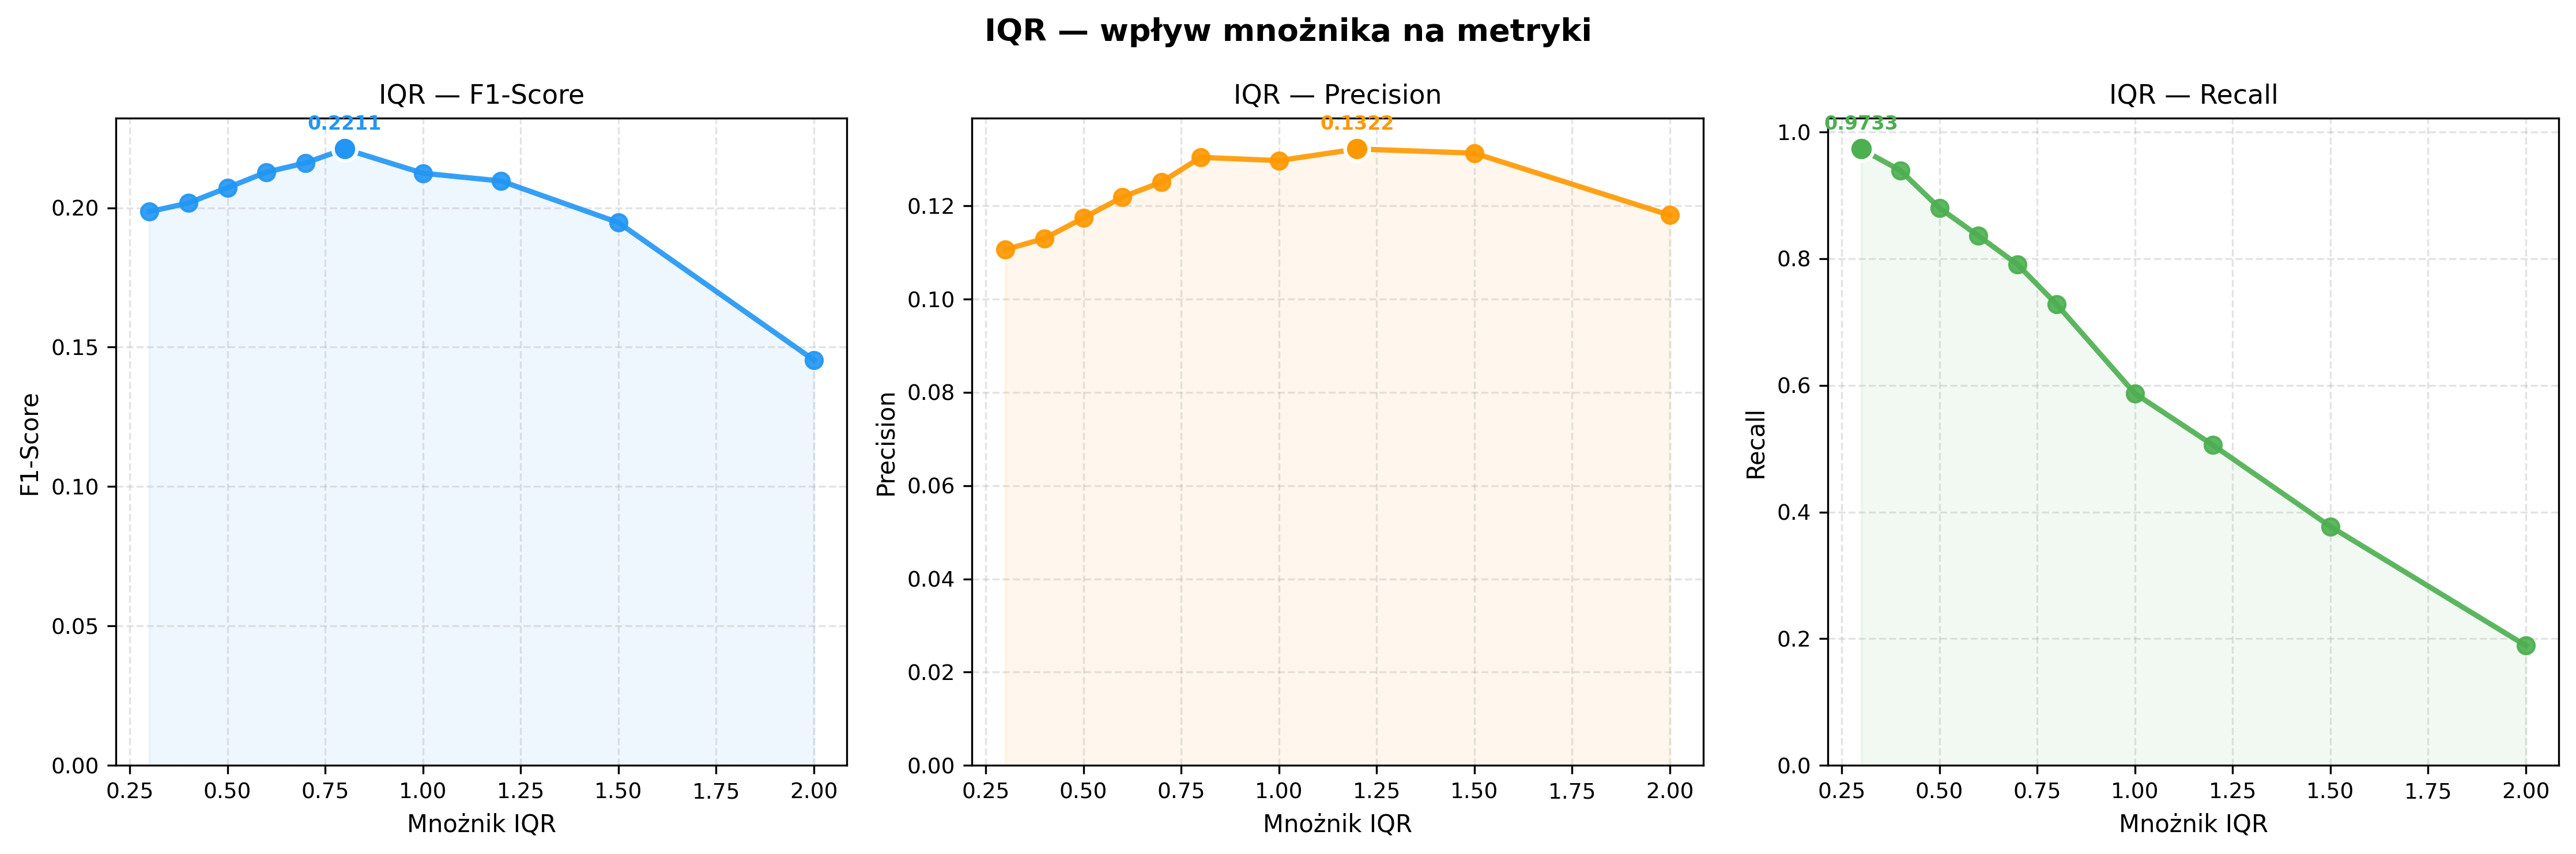
\includegraphics[width=0.9\textwidth]{fig_02b_iqr_params.png}
		\caption{Wpływ mnożnika na metryki detekcji w metodzie IQR}
		\label{fig:02b-iqr-params}
	\end{figure}
	
	\subsection{Metoda Z-Score}
	Metoda Z-Score działa poprzez normalizację każdej z cech w odniesieniu do jej rozkładu w zbiorze treningowym i klasyfikuje próbkę jako anomalię, jeżeli któraś z cech przekracza próg ~$\theta$ w jednostkach odchylenia standardowego. Wartości progu testowane w ramach badań zawierały się w przedziale od 0.2 do 3.0
	\begin{figure}%[H]
		\centering
		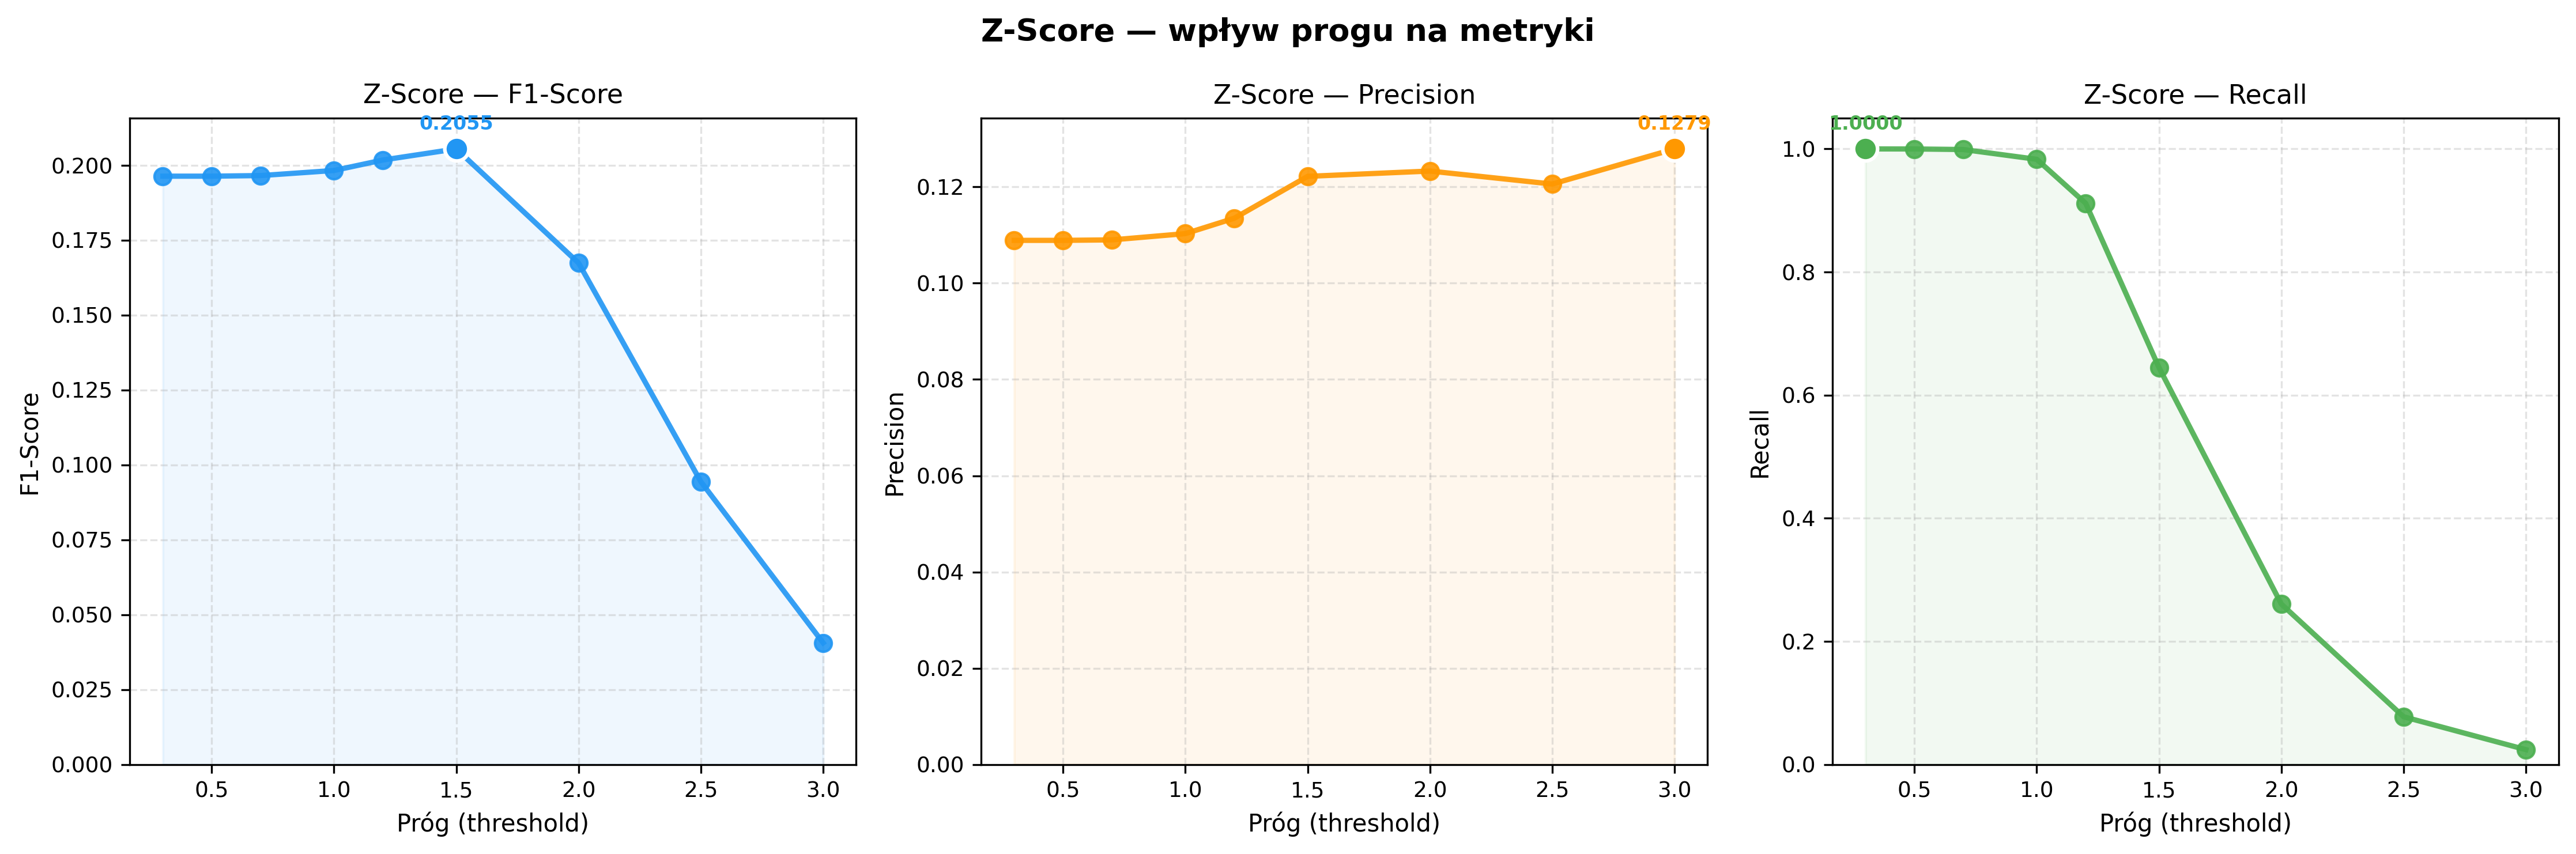
\includegraphics[width=0.9\textwidth]{fig_02b_zscore_params.png}
		\caption{Wpływ progu odcięcia na metryki detekcji w metodzie Z-Score}
		\label{fig:02b-zscore-params}
	\end{figure}
	Rysunek \ref{fig:02b-zscore-mod-params}, który prezentuje wyniki strojenia parametru, ukazuje podobne wyniki jak w przypadku punktu odniesienia, gdyż w początkowych wartościach, do 1.0 wartości trzymają swój poziom, który charakteryzuje się, ponownie, niską precyzją, co oznacza dużą ilość fałszywych alarmów, ale bardzo wysoką, a momentami nawet perfekcyjną, czułością, czyli wszystkie anomalie zostały wykryte w szeregu czasowym testowanym na potrzeby tego badania. Natomiast, po przekroczeniu progu 1.0 czułość rozpoczęła gwałtowny spadek, który trwał do końca badania tej metody. Zjawiskiem przyciągającym uwagę jest nieznaczne zwiększenie precyzji proporcjonalnie do progu, lecz tempo wzrostu nie odpowiada spadkowi czułości, co czyni tą poprawę mało istotną w kontekście F1-Score. Kompromisem zmian tych parametrów okazała się konfiguracja z wartością progu równą 1.5, która dała wynik F1 równy 0{,}2055, który okazał się słabszy od punktu bazowego o około pół procenta. Obie metody działają w podobny sposób, gdzie jedyną różnicą jest miara rozproszenia (IQR i odchylenie standardowe). 
	
	\subsection{Zmodyfikowana metoda Z-Score}
	Zmodyfikowana metoda Z-Score od standardowej różni się zamianą średniej stosuję medianę. Odchylenie standardowe zastąpione jest medianą bezwzględnych odchyleń (MAD). Zmiany te dają większą odporność na skrajne wartości, które występują w zbiorze treningowym. 
	
	\begin{figure}%[H]
		\centering
		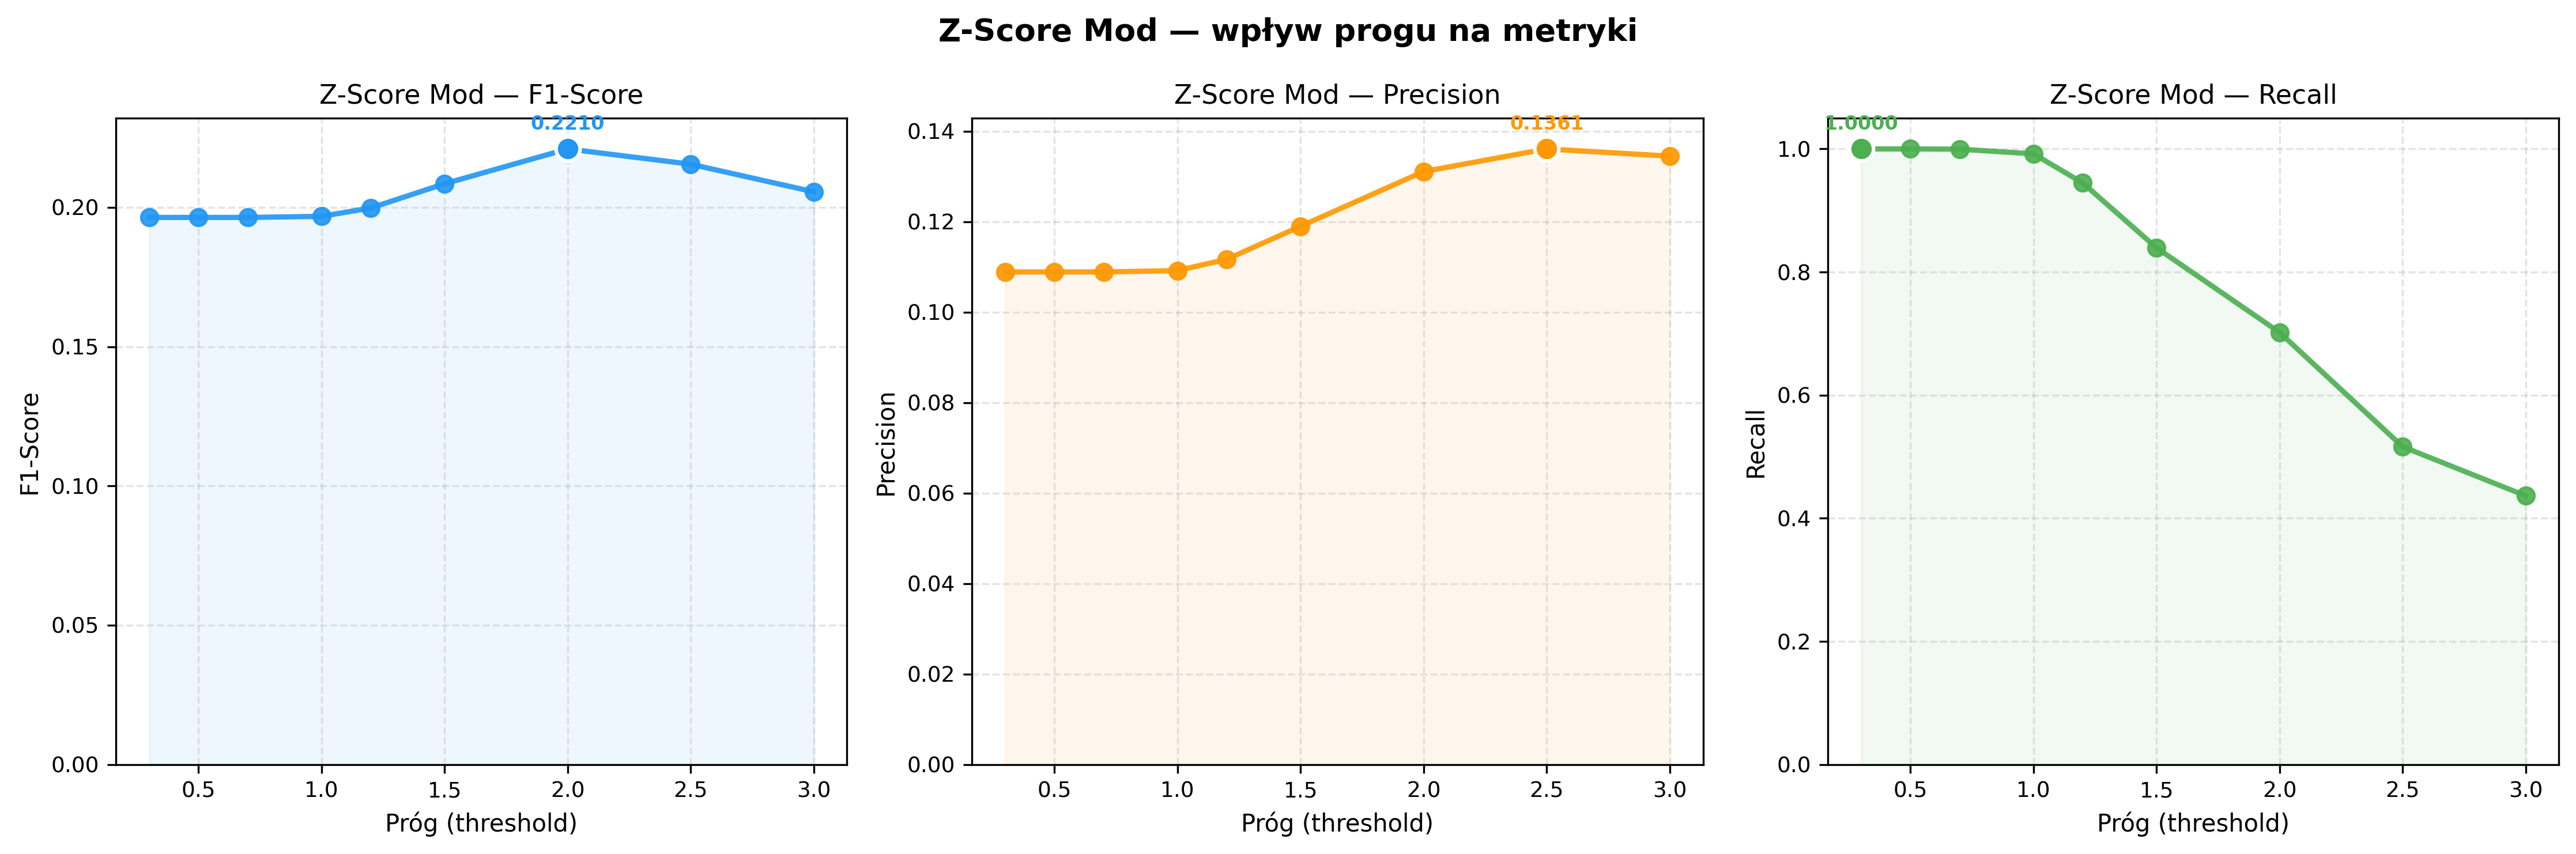
\includegraphics[width=0.9\textwidth]{fig_02b_zscore_mod_params.png}
		\caption{Wpływ progu odcięcia na metryki detekcji w zmodyfikowanej metodzie Z-Score}
		\label{fig:02b-zscore-mod-params}
	\end{figure}
	
	Wyniki, które przedstawia rysunek \ref{fig:02b-zscore-mod-params} charakter zmian wartości miar (które były testowane na tym samym zbiorze parametrów, co standardowa metoda), są podobne co do poprzedniej metody. Natomiast wzrost precyzji jest większy,  a spadek czułości znacznie mniejszy, gdyż najgorsza wartość progu powoduje czułość na poziomie około 40 \%, czyli dwa razy większym niż w przypadku oryginalnej metody Z-Score. Natomiast, nawet przy tych poprawkach, wartość F1 wynosi 0{,}2210, co oznacza, że w porównaniu do punktu odniesienia metoda ta jest gorsza o~0{,}0001 punktu F1, która jest na tyle małą liczbą, że można uznać tą różnicę za nieistotną i przyjąć metodę za równą odniesieniu.
	
	\subsection{CUSUM}
	Metoda CUSUM działa na mechanizmie pamięci, która zapisuje skumulowane odchylenia, co powoduje, że nakładanie cech z mechanizmu okna kroczącego jest zbędne, gdyż ich dodanie powoduje zamieszanie i niezdolność algorytmu do dochodzenia do rozsądnych wyników. W eksperymentach dla tej metody dobierano dwa parametry. Pierwszy ~$h$ to próg decyzji, a drugi ~$k$ oznacza dryf, kontrolujący wrażliwość na zmienność sygnału. Wartości te były sprawdzane w parach próg równy 0.001 i dryft 0.0001 i proporcjonalnie zwiększane do poziomu progu 0.1.
	
	\begin{figure}%[H]
		\centering
		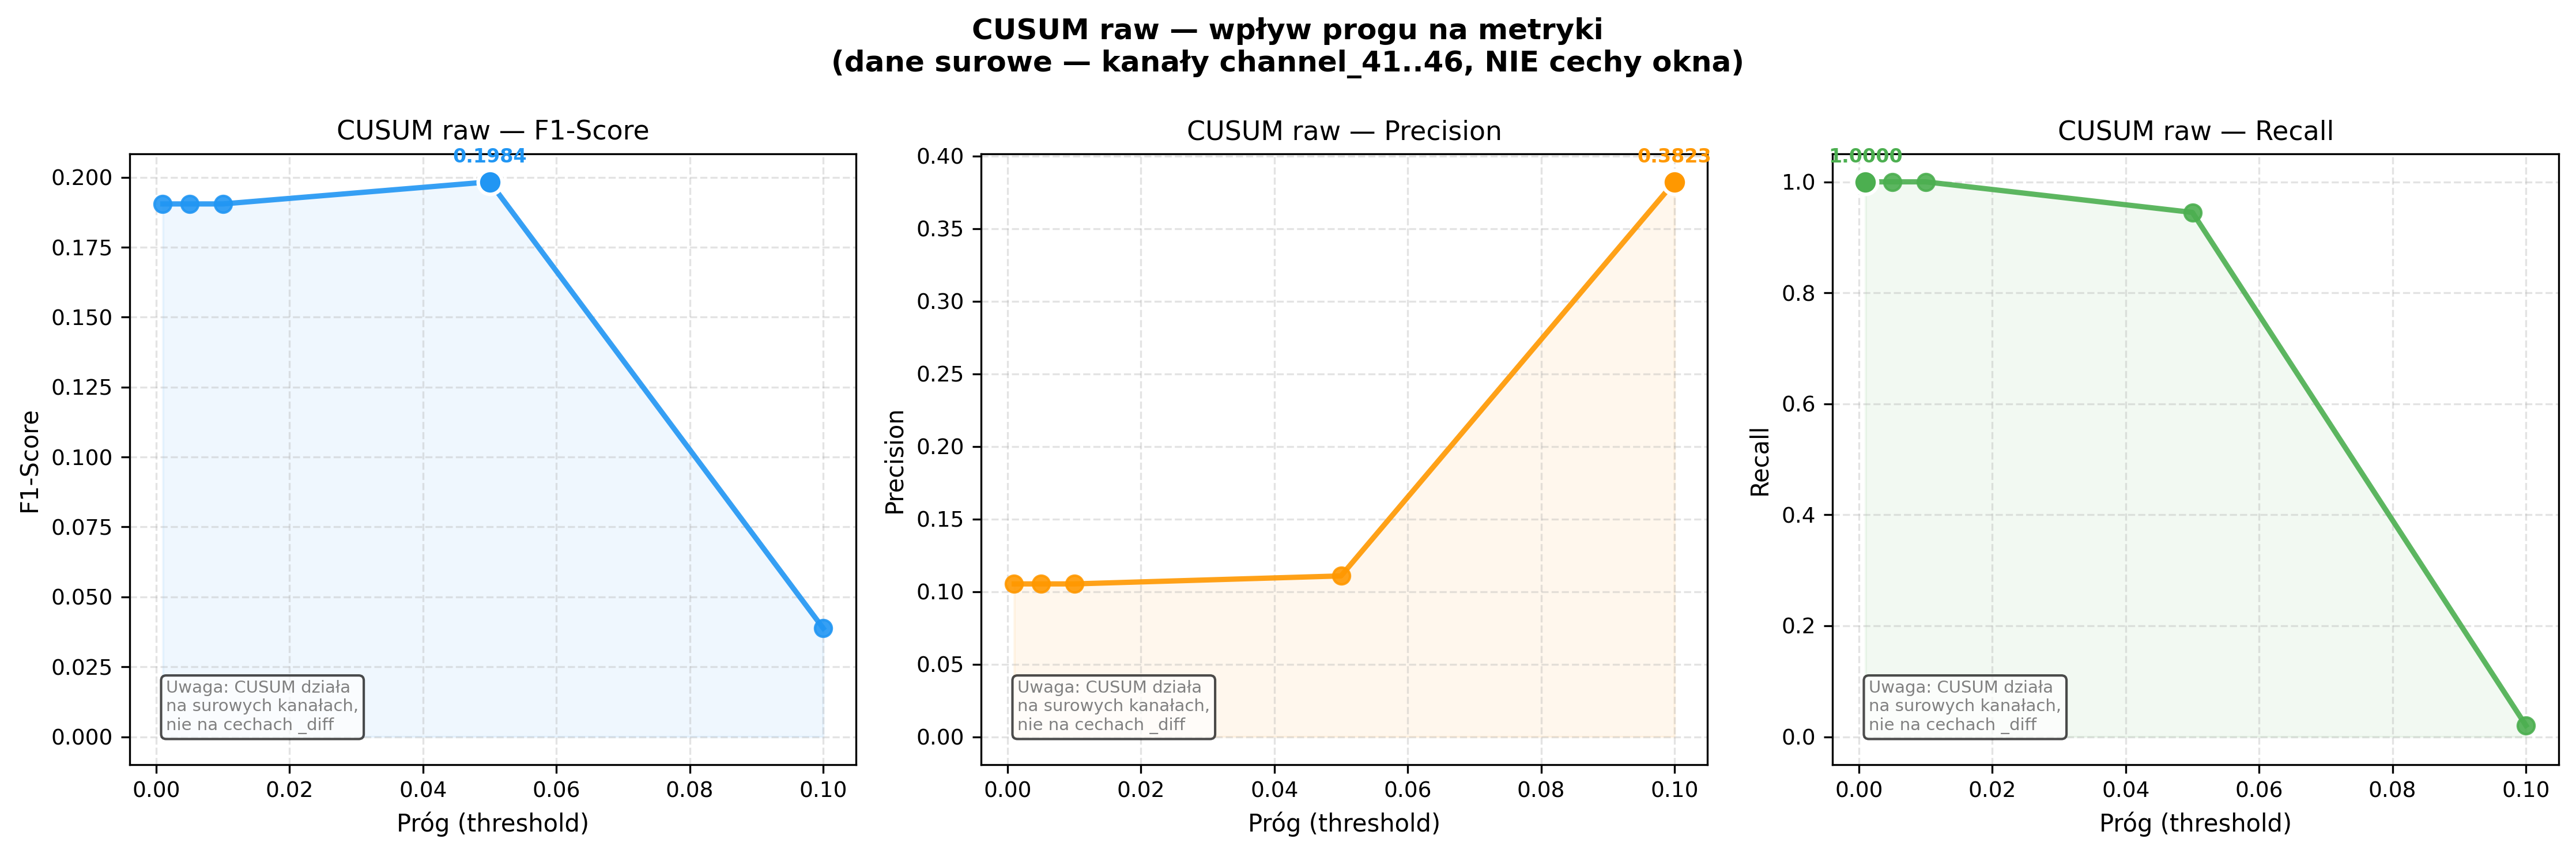
\includegraphics[width=0.9\textwidth]{fig_02b_cusum_raw_params.png}
		\caption{Wpływ progu detekcji na metryki w metodzie CUSUM na surowych danych.}
		\label{fig:02b-cusum_raw-params}
	\end{figure}
	
	Rysunek \ref{fig:02b-cusum_raw-params} ukazuje wyniki testowania metody, które są odzwierciedleniem metody CUSUM, jak i całej grupy metod statystycznych, czyli czułość ciągle zwiększająca się do bardzo wysokich poziomów sięgających 0{,}9449, przy najniższej w badaniu precyzji na poziomie 0{,}1108, co daje F1 na poziomie 0{,}1984. Poprzez akumulację odchyleń w czasie, w przypadku pojawienia się anomalii sumy kumulowane się zwiększają na kolejne próbki, co powoduje zwiększenie fałszywych alarmów w okolicach anomalii. Przy niskich wartościach parametrów jest to szczególne widoczne w wynikach.
	
	\subsection{EWMA}
	Wykładniczo ważona średnia ruchoma (EWMA) dokonuje dopasowania poziomu referencyjnego sygnału, które jest regulowane przez parametr \textit{span}. Anomalia zostaje wykryta, gdy wartość cechy odbiega od wygładzonej średniej o więcej niż $\theta$ lokalnych odchyleń standardowych okna. W eksperymencie testowano oba parametry. 
	
	\begin{figure}%[H]
		\centering
		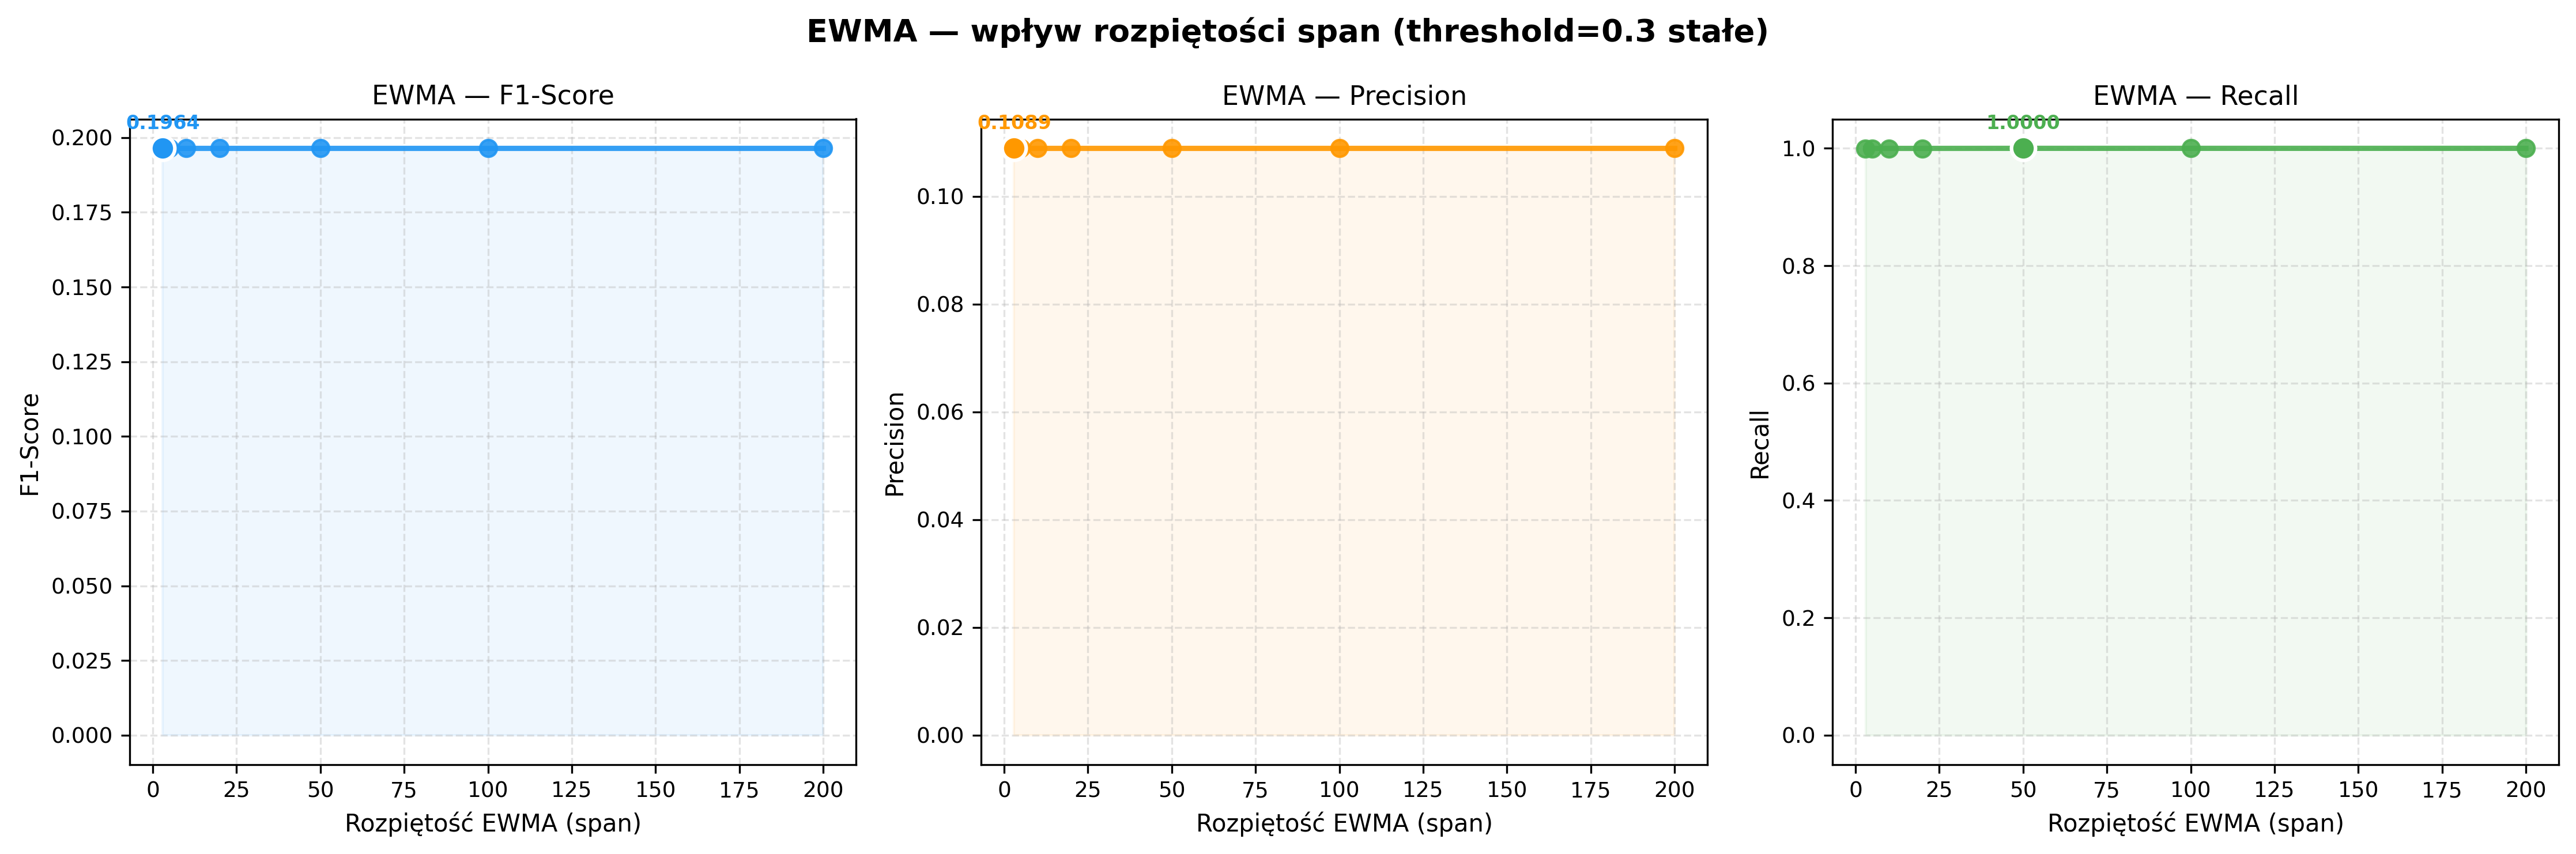
\includegraphics[width=0.9\textwidth]{fig_02b_ewma_span.png}
		\caption{Wpływ parametru rozpiętości na metryki w metodzie EWMA.}
		\label{fig:02b-ewma-span}
	\end{figure}
	\begin{figure}%[H]
		\centering
		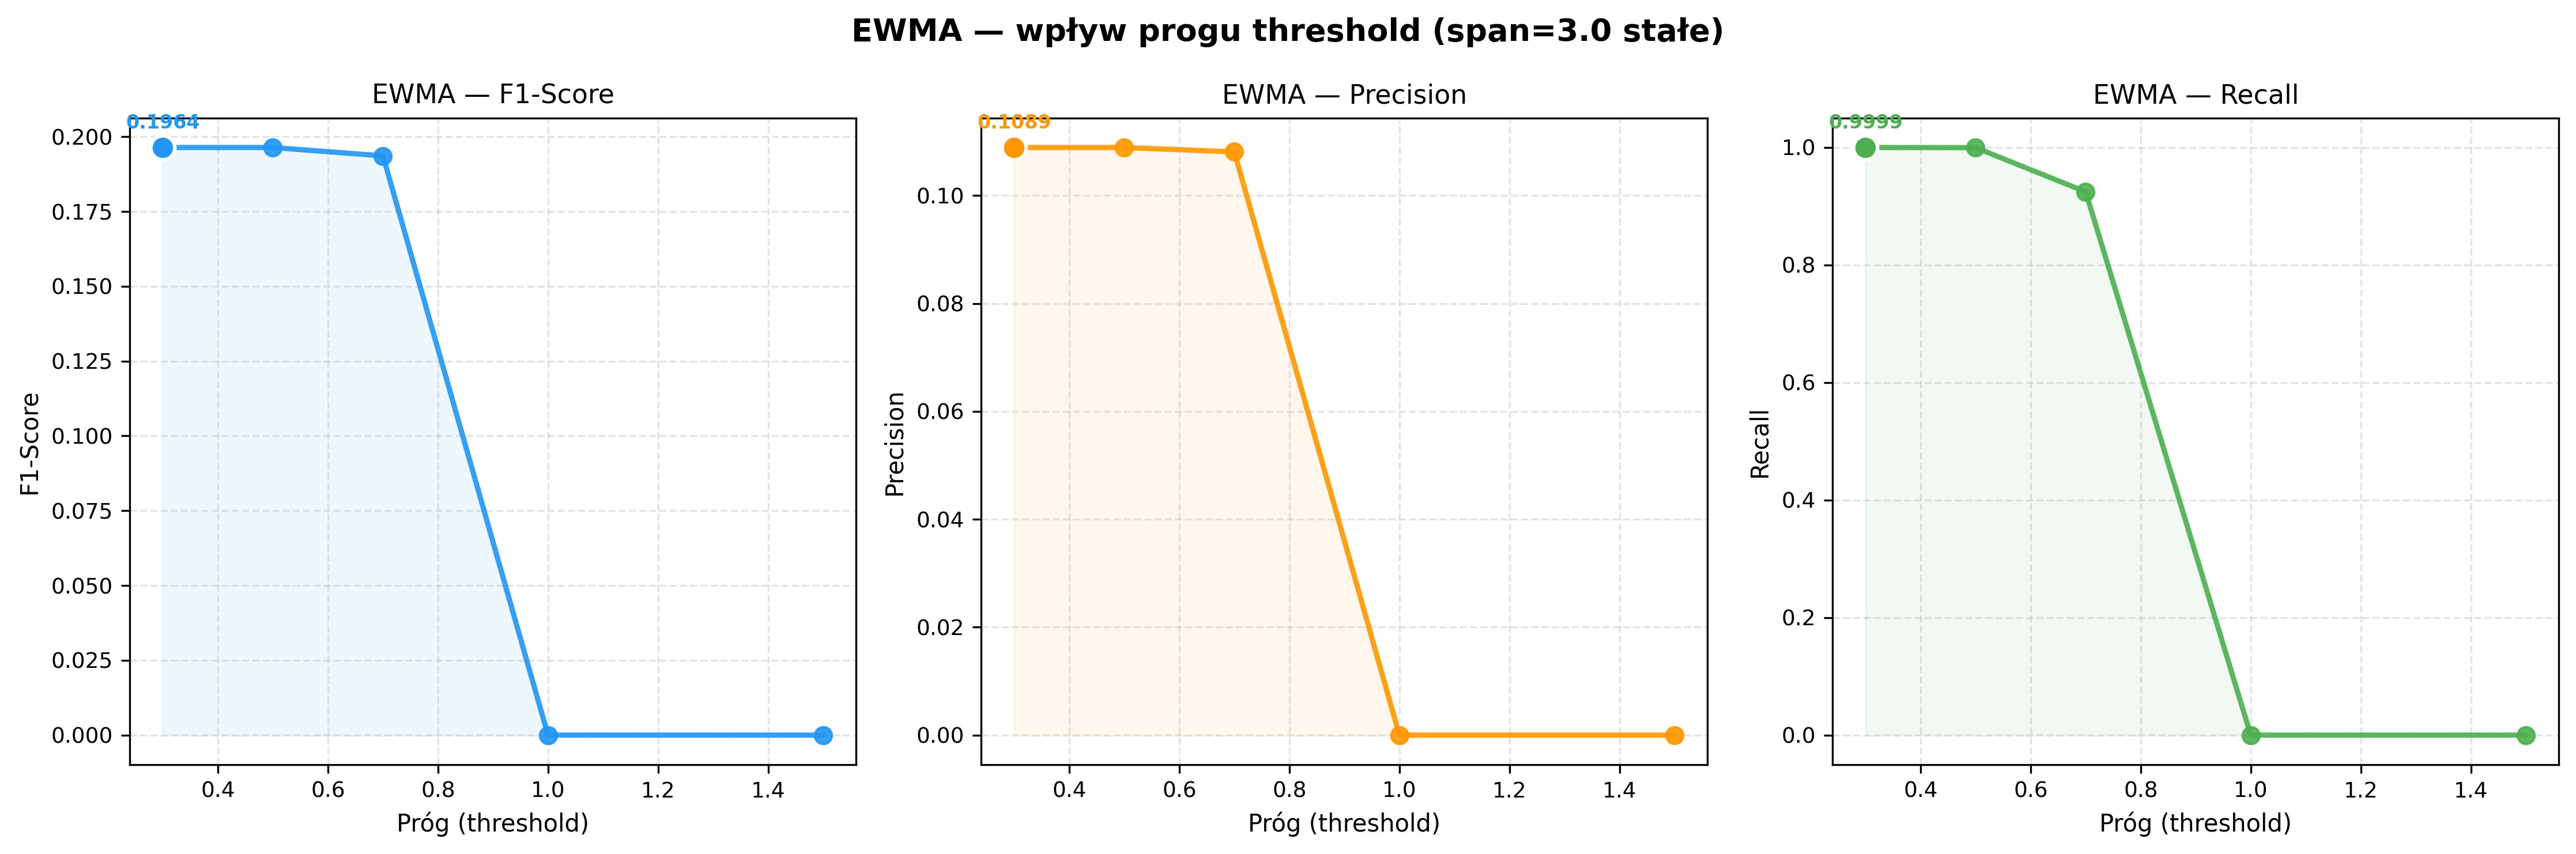
\includegraphics[width=0.9\textwidth]{fig_02b_ewma_threshold.png}
		\caption{Wpływ progu odcięcia na metryki w metodzie EWMA.}
		\label{fig:02b-ewma-threshold}
	\end{figure}
	
	Rysunek \ref{fig:02b-ewma-span} ukazuje duży problem algorytmu opartego na cechach, jakakolwiek zmiana parametru \text{span}  w zakresie od 3 do 200 nie ma żadnego wpływu na wyniki. Wszystkie trzy miary nie zmieniają swojej wartości zależnie od parametru span. F1-Score zatrzymuje się na płaskim poziomie 0{,}1964, pomimo tego, że wszystkie anomalie zostały wykryte, gdyż czułość wynosiła 1.0. Te zjawisko, po części wyjaśnia rysunek \ref{fig:02b-ewma-threshold}, który pokazuje, że dla wartości $span = 3$ nawet niskie wartości progu nie poprawiają wyników, a powyżej progu 0.7 model przestaje wykrywać anomalie. Brak wrażliwości na parametr \text{span} i wąski zakres użyteczności progu, wynika z cechy \text{diff} okna kroczącego, która jest już wycentrowana przez to okno, jednocześnie negując mechanizm EWMA.  Najlepszym wynik działania algorytmu okazał się F1\,=\,0{,}1964
	
	\subsection{Podsumowanie wyników metod statystycznych}
	Rysunek \ref{fig:02b-summary-comparison} zestawia ze sobą wszystkie najlepsze konfiguracje parametrów, dla każdej z ewaluowanych metod. Żadna z testowanych metod nie poprawiła wartości F1 punktu odniesienia. Jedną rzeczą, która charakteryzuje całokształt wyników, jest brak równowagi pomiędzy precyzją, a czułością, co ma duży wpływ na wartość F1. Wyniki wszystkich metod nie różnią się znacznie między sobą, między najlepszą (IQR, F1\,=\,0{,}2211), a najgorszą (EWMA, F1\,=\,0{,}1964) metodą jest tylko 0.0247 punktu F1 różnicy. Ograniczenie skuteczności leży nie w doborze metody, ale w naturze progowania jednowymiarowego.
	
	\begin{figure}%[H]
		\centering
		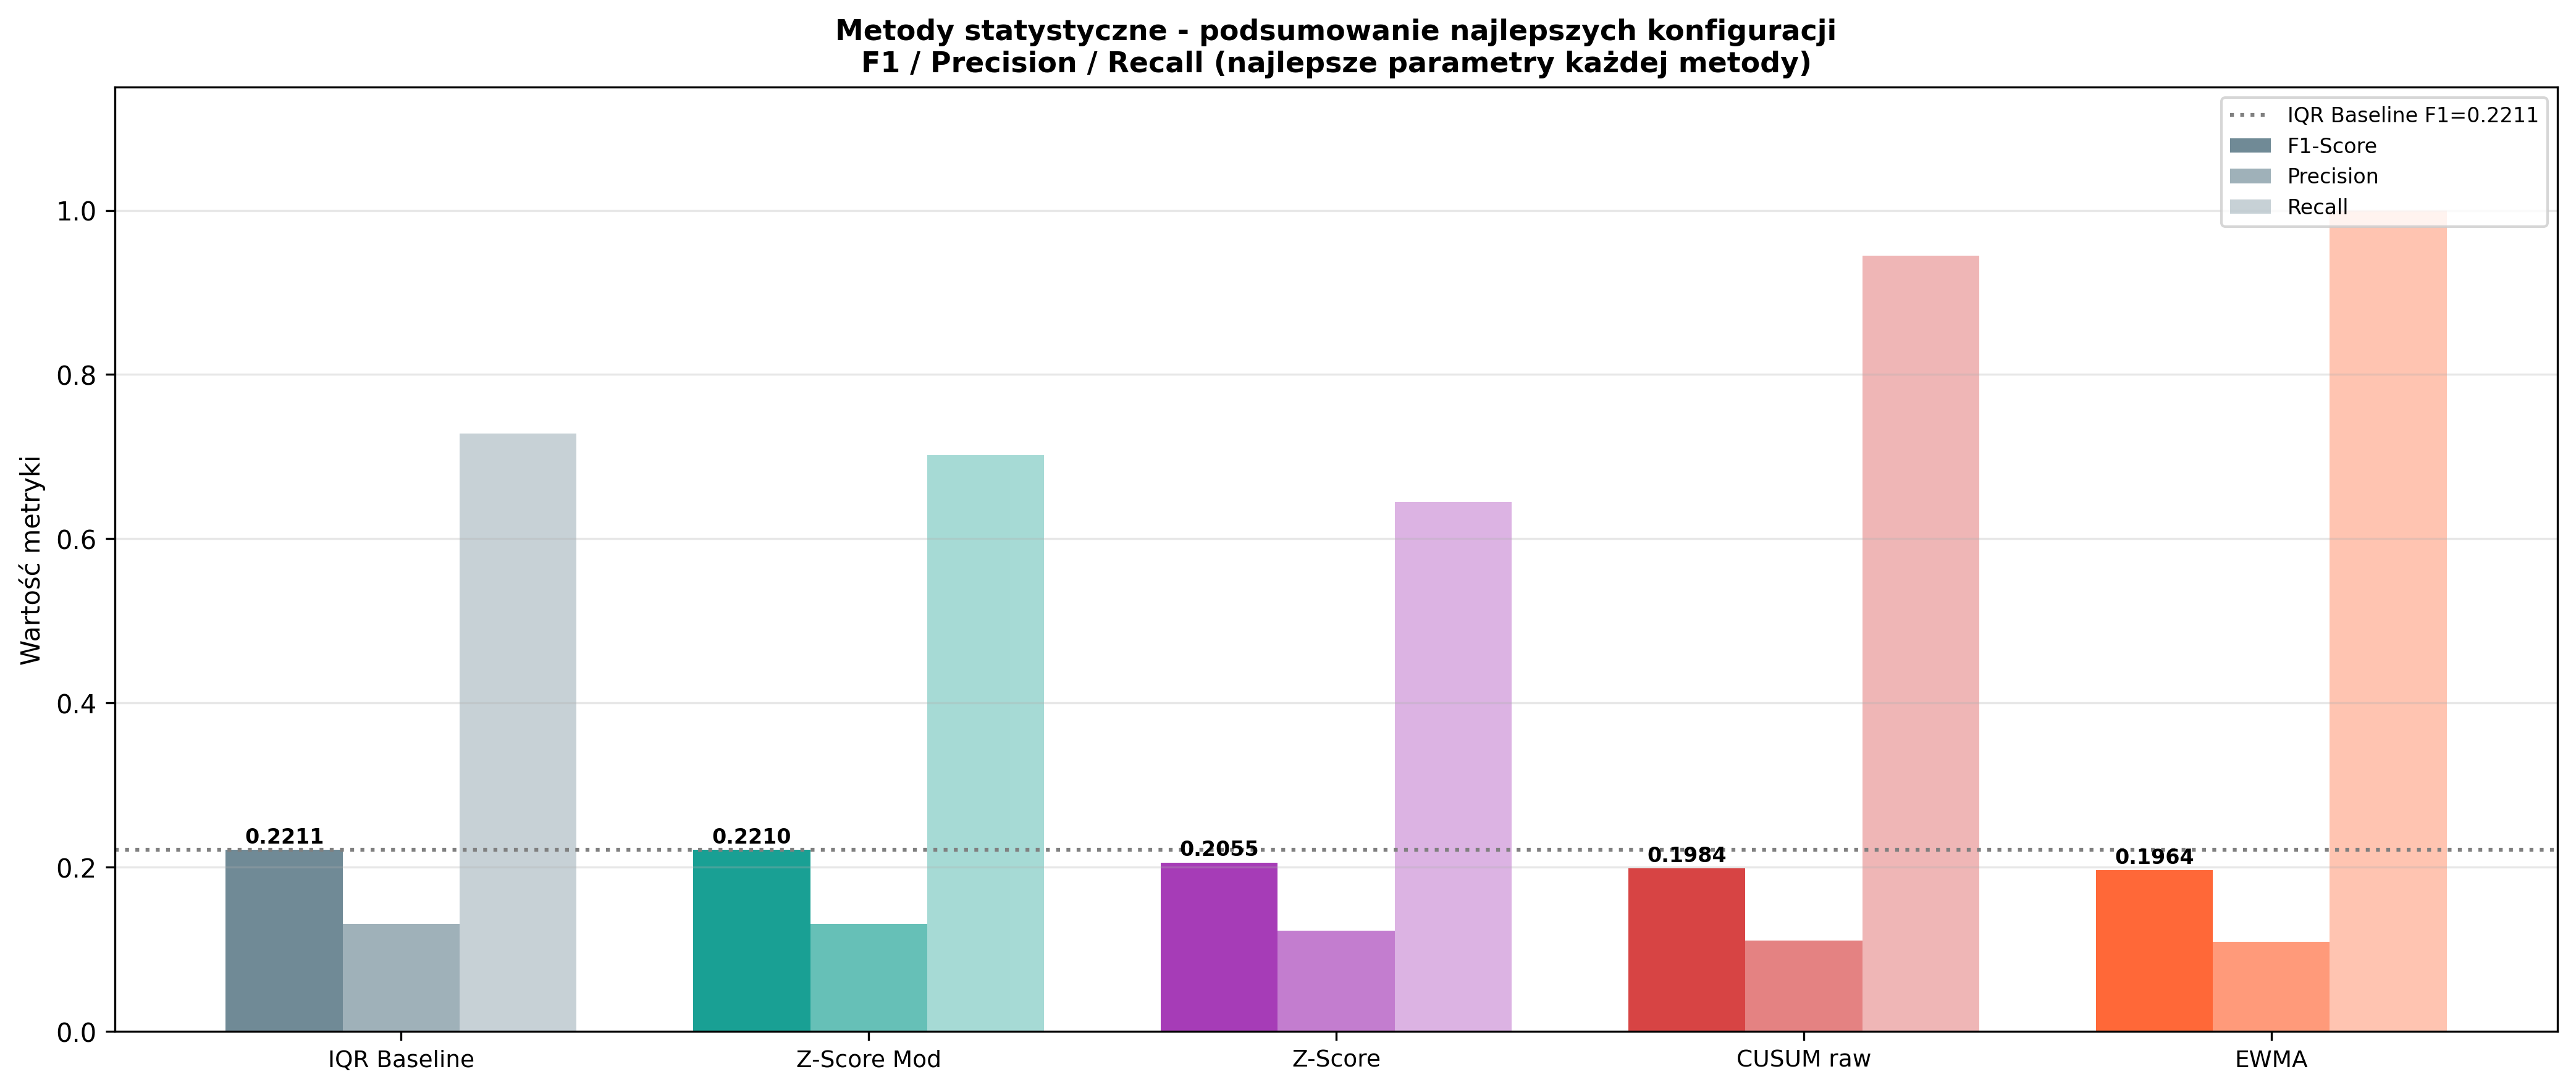
\includegraphics[width=0.9\textwidth]{fig_02b_summary_comparison.png}
		\caption{Porównanie metryk uzyskanych przez metody statystyczne z pierwszym progiem}
		\label{fig:02b-summary-comparison}
	\end{figure}
	
	\section{Wyniki metod uczenia maszynowego}
	Tak jak w przypadku metod statystycznych, algorytmy uczenia maszynowego wykorzystują ten sam zestaw cech wyznaczonych przez mechanizm okna kroczącego. Dodatkowo przed rozpoczęciem eksperymentu badawczego zastosowano standaryzację Z-Score (\texttt{StandardScaler}) wyznaczoną na danych oznaczonych jako normalne w zbiorze treningowym. W przypadku metod uczenia maszynowego należy zwrócić uwagę na dużą złożoność obliczeniową algorytmów Local Outlier Factor i One-Class SVM. Aby uniknąć zawieszenia systemu konieczne było ograniczenie próbki treningowej do odpowiednio 50 i 20 tysięcy próbek, co jest bardzo małą liczbą, biorąc pod uwagę fakt, że zbiór testowy posiada kilkanaście milionów danych w sobie. Pomimo faktu dużej redukcji danych do treningu, model był testowany na pełnym zestawie danych testowych. 
	
	\subsection{Isolation Forest}
	Algorytm Isolation Forest, zwany także lasem izolacji działa poprzez losowe dzielenie przestrzeni cech na niezależne obszary, w celu odizolowania anomalii. W momencie, jeżeli dany punkt potrzeba wyraźnie mniejszej liczby podziałów do wyróżnienia, jest uznawany wtedy za anomalię. W ramach strojenia modelu, modyfikowanymi parametrami były \textit{contamination}, które określa oczekiwany odsetek anomalii w zbiorze treningowym w zakresie od 0{,}08 do 0{,}3, a także ilość drzew, które losowo dzielą dane. Rozważano przypadek 100, 200 i 300 takich estymatorów.
	
	\begin{figure}%[H]
		\centering
		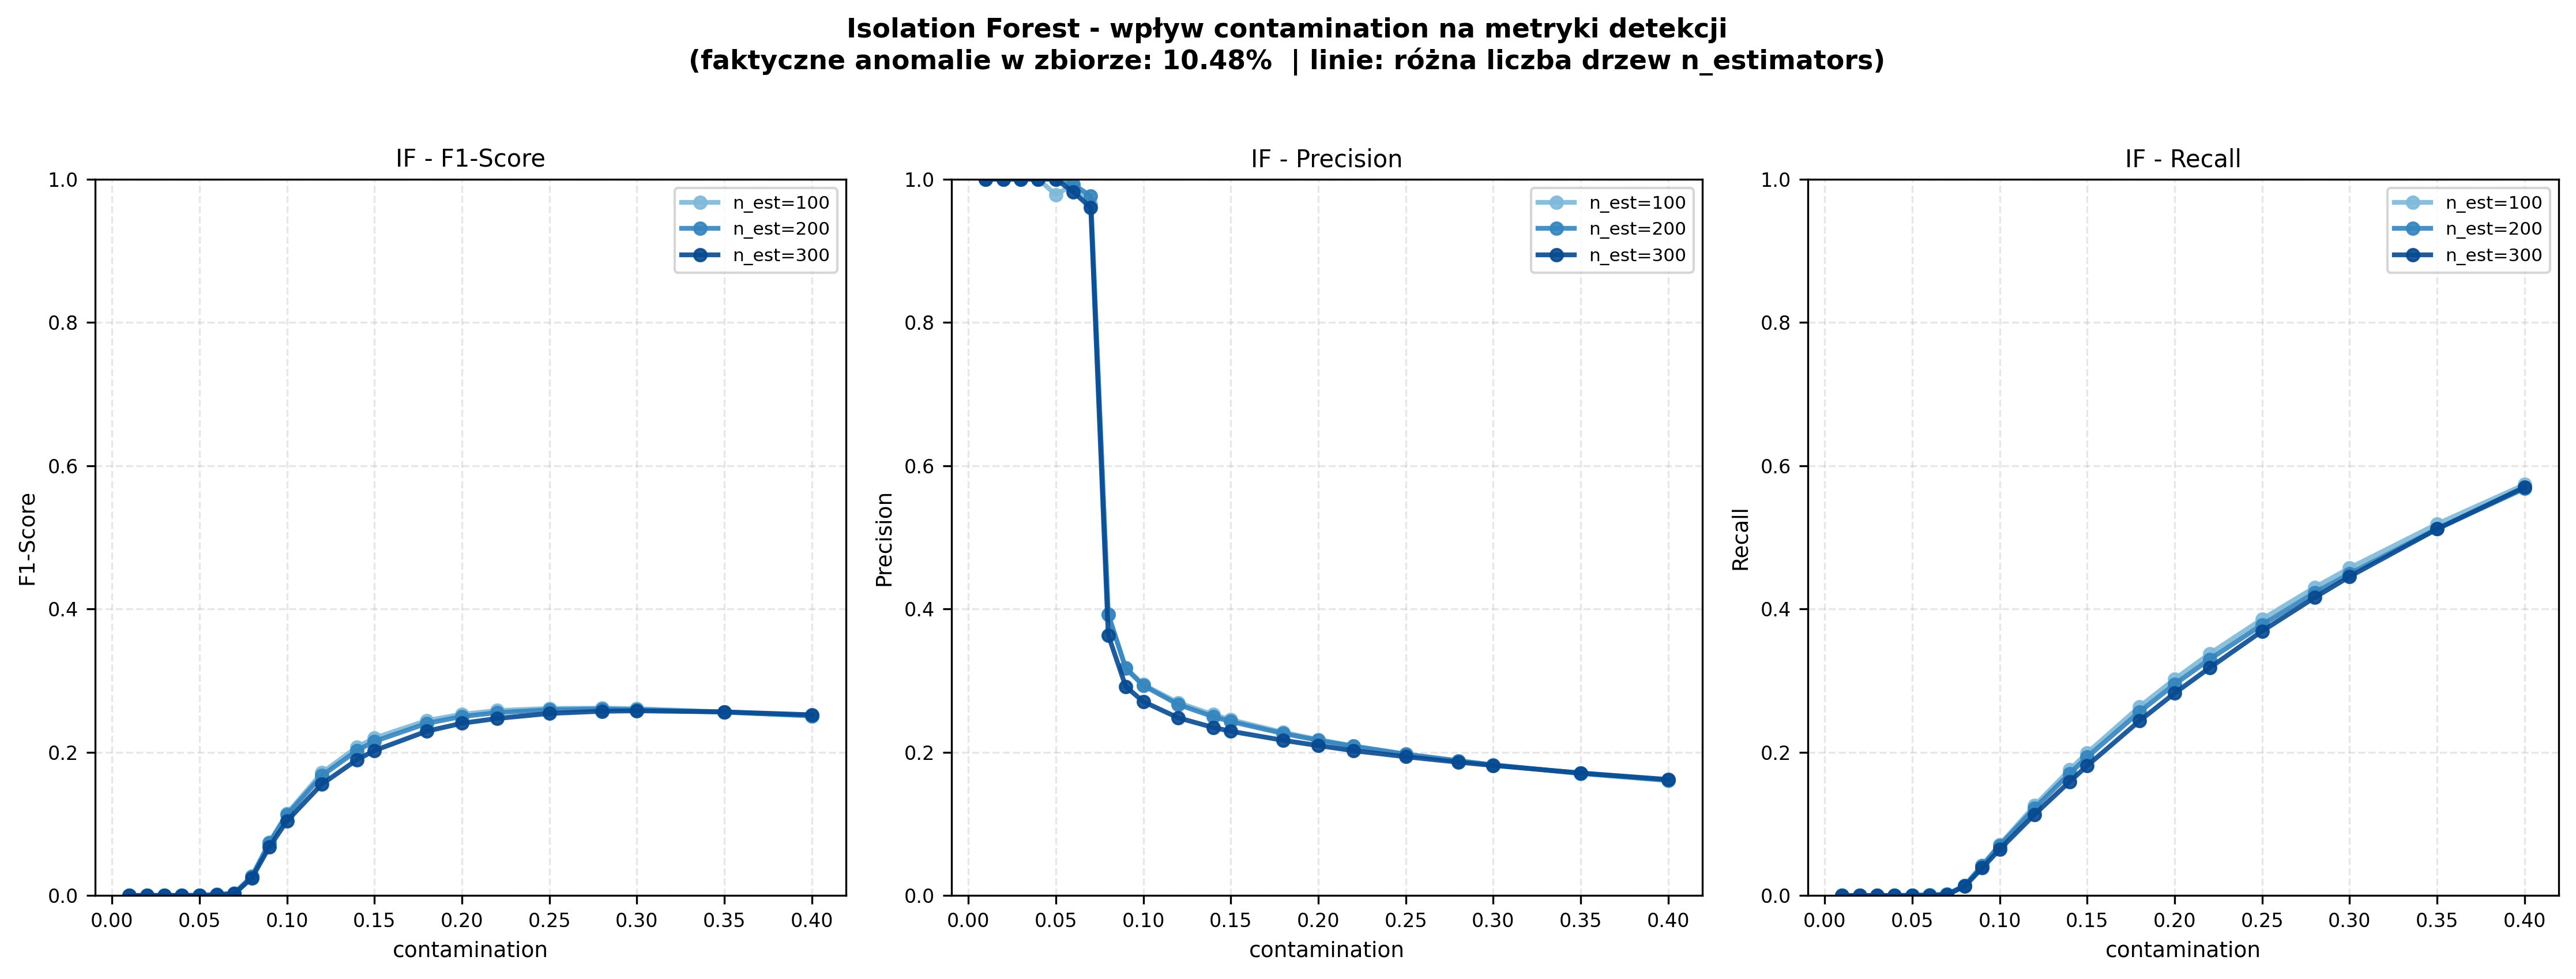
\includegraphics[width=0.9\textwidth]{fig_03b_if_params_v4.png}
		\caption{Wpływ parametru contamination na metryki detekcji w algorytmie Isolation Forest}
		\label{fig:03b-if-params}
	\end{figure}
	\begin{figure}%[H]
		\centering
		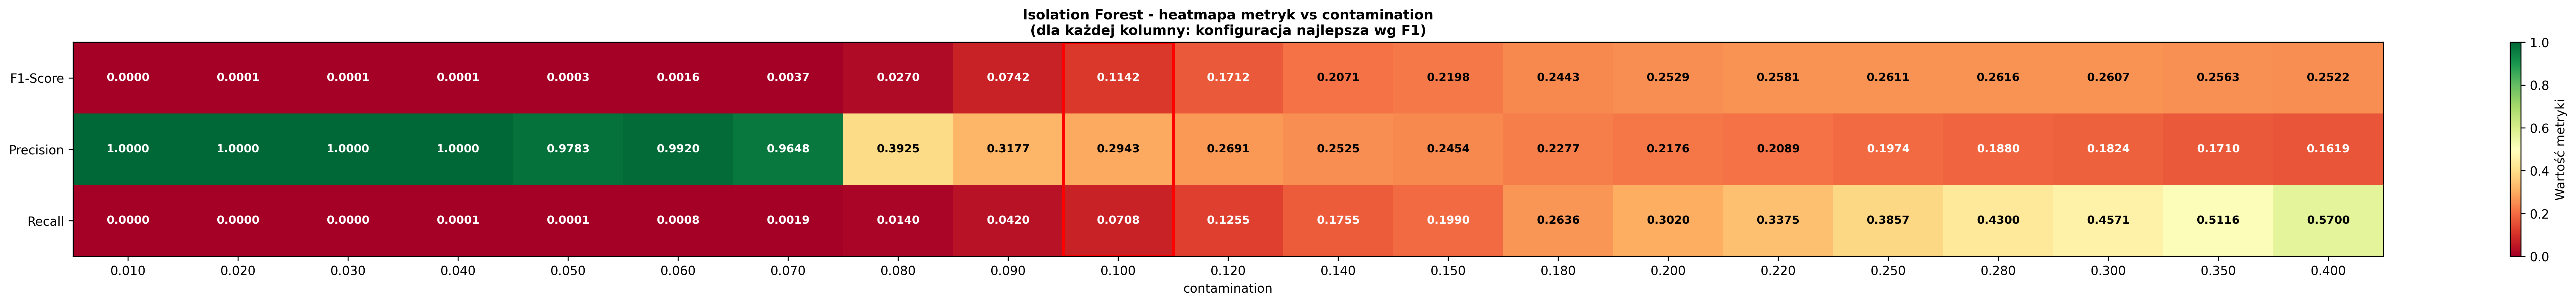
\includegraphics[width=0.9\textwidth]{fig_03b_isolation_forest_heatmap_v2.png}
		\caption{Macierz korelacji metryk z parametrem contamination(WIP) w algorytmie Isolation Forest}
		\label{fig:03b-isolation-forest-heatmap}
	\end{figure}
	
	Rysunek \ref{fig:03b-if-params} prezentuje wyniki  badania wpływu parametrów na wyniki, z zaznaczonym faktycznym udziałem anomalii w zbiorze testowym. Zerowe wyniki czułości dla najmniejszej wartości \textit{contamination} powoduje pozornie idealną precyzję z powodu małej ilości faktycznych wykrytych anomalii, na co wskazuje czułość. Dopiero w miarę zwiększenia wartości parametru wyniki F1 zaczęły się poprawiać  Wbrew intuicji najlepszą konfiguracją okazała się ta z parametrem \textit{contamination} równym 0{,}28, która zakładała większego udziału anomalii w zbiorze, niż faktycznie jest. W przedziale największych parametrów testowanych wynik F1 zaczął się stabilizować, gdyż prędkość spadku precyzji zmniejszyła się, natomiast wyniki czułości dalej rosły w miarę stablinym tempie. Wykresy te pokazują, że wpływ liczby drzew był widoczny tylko dla małych wartości parametru \textit{contamination}, co czyniło ten estymator drugorzędnym w ewaluacji. Najlepszą, pod względem wyniku miary F1-Score, konfiguracją okazała się ta, z \textit{contamination} równym 0.25 dla 100 drzew. F1 wyniosło dla tego zestawu 0{,}2616., przy precyzji wynoszącej 0{,}1880 i czułości na poziomie 0{,}4300. Wyniki dla konfiguracji parametru contamination przentuje heatmapa na rysunku \ref{fig:03b-isolation-forest-heatmap}, gdzie czerwoną ramką zaznaczono wyniki dla parametru \textit{contamination}, który jest najbliżej faktycznego procentu anomalii w zbiorze testowym. 
	
	\subsection{Local Outlier Factor}
	Algorytm LOF działa poprzez mierzenie  gęstości punktu w stosunku do jego sąsiadów, czyli odległość do najbliższych punktów w okolicy próbki badanej. Dane, które znalazły się w znacznej odległości od swoich najbliższych sąsiednich punktów, są uznawane za anomalie. W ramach tej metody testowano, tak jak w przypadku poprzedniej, dwa parametry. Pierwszym z nich była liczba najbliższych sąsiadów $k$ do mierzenia odległości od badanego punktu w zakresie od 3 do 50. Drugim parametrem, był znany z poprzedniej metody \textit{contamination}. 
	\begin{figure}%[H]
		\centering
		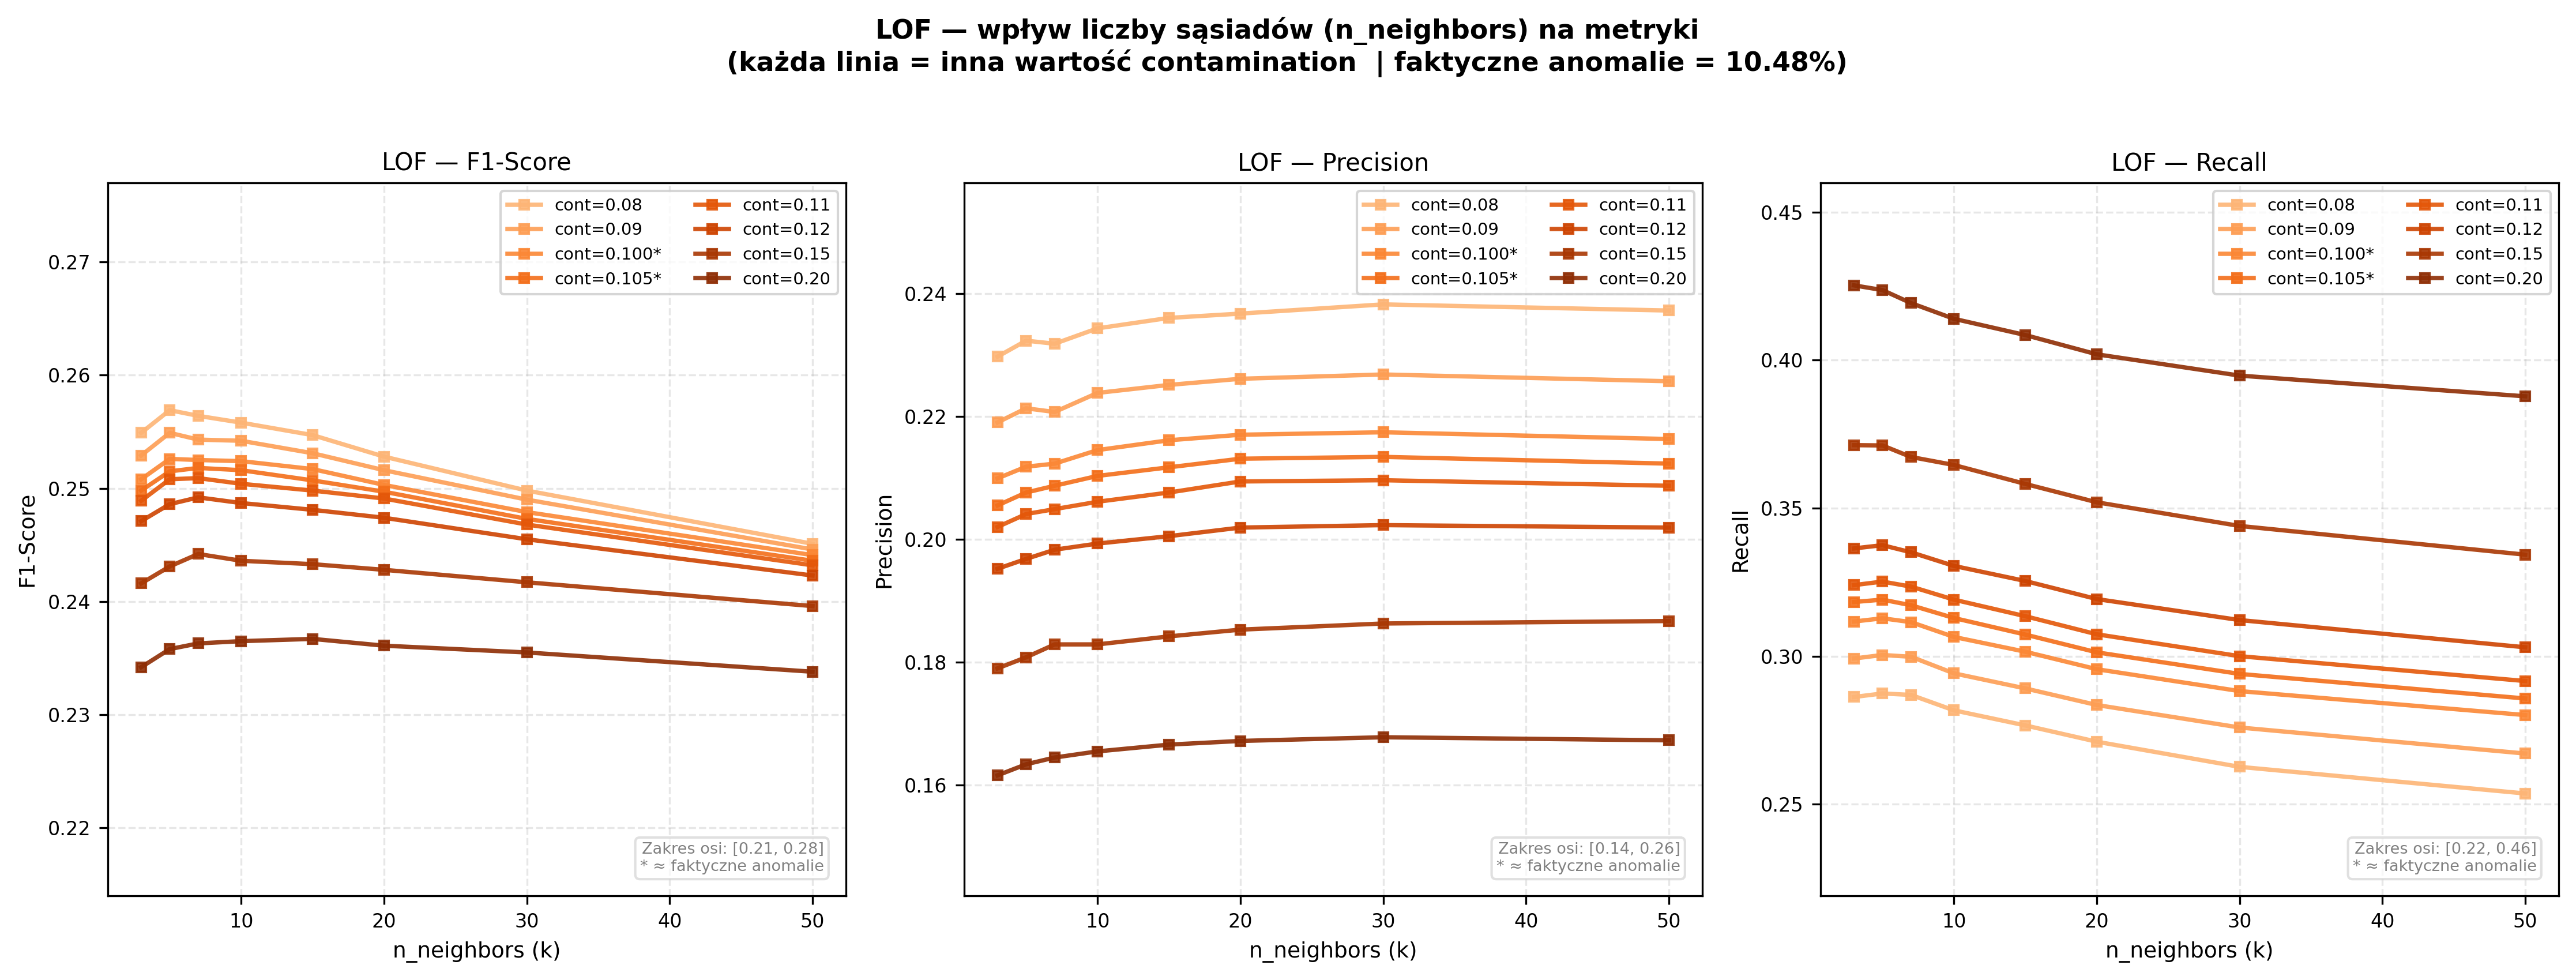
\includegraphics[width=0.9\textwidth]{fig_03b_lof_params_v4.png}
		\caption{Wpływ liczby sąsiadów na metryki detekcji w algorytmie Local Outlier Factor}
		\label{fig:03b-lof-params}
	\end{figure}
	\begin{figure}%[H]
		\centering
		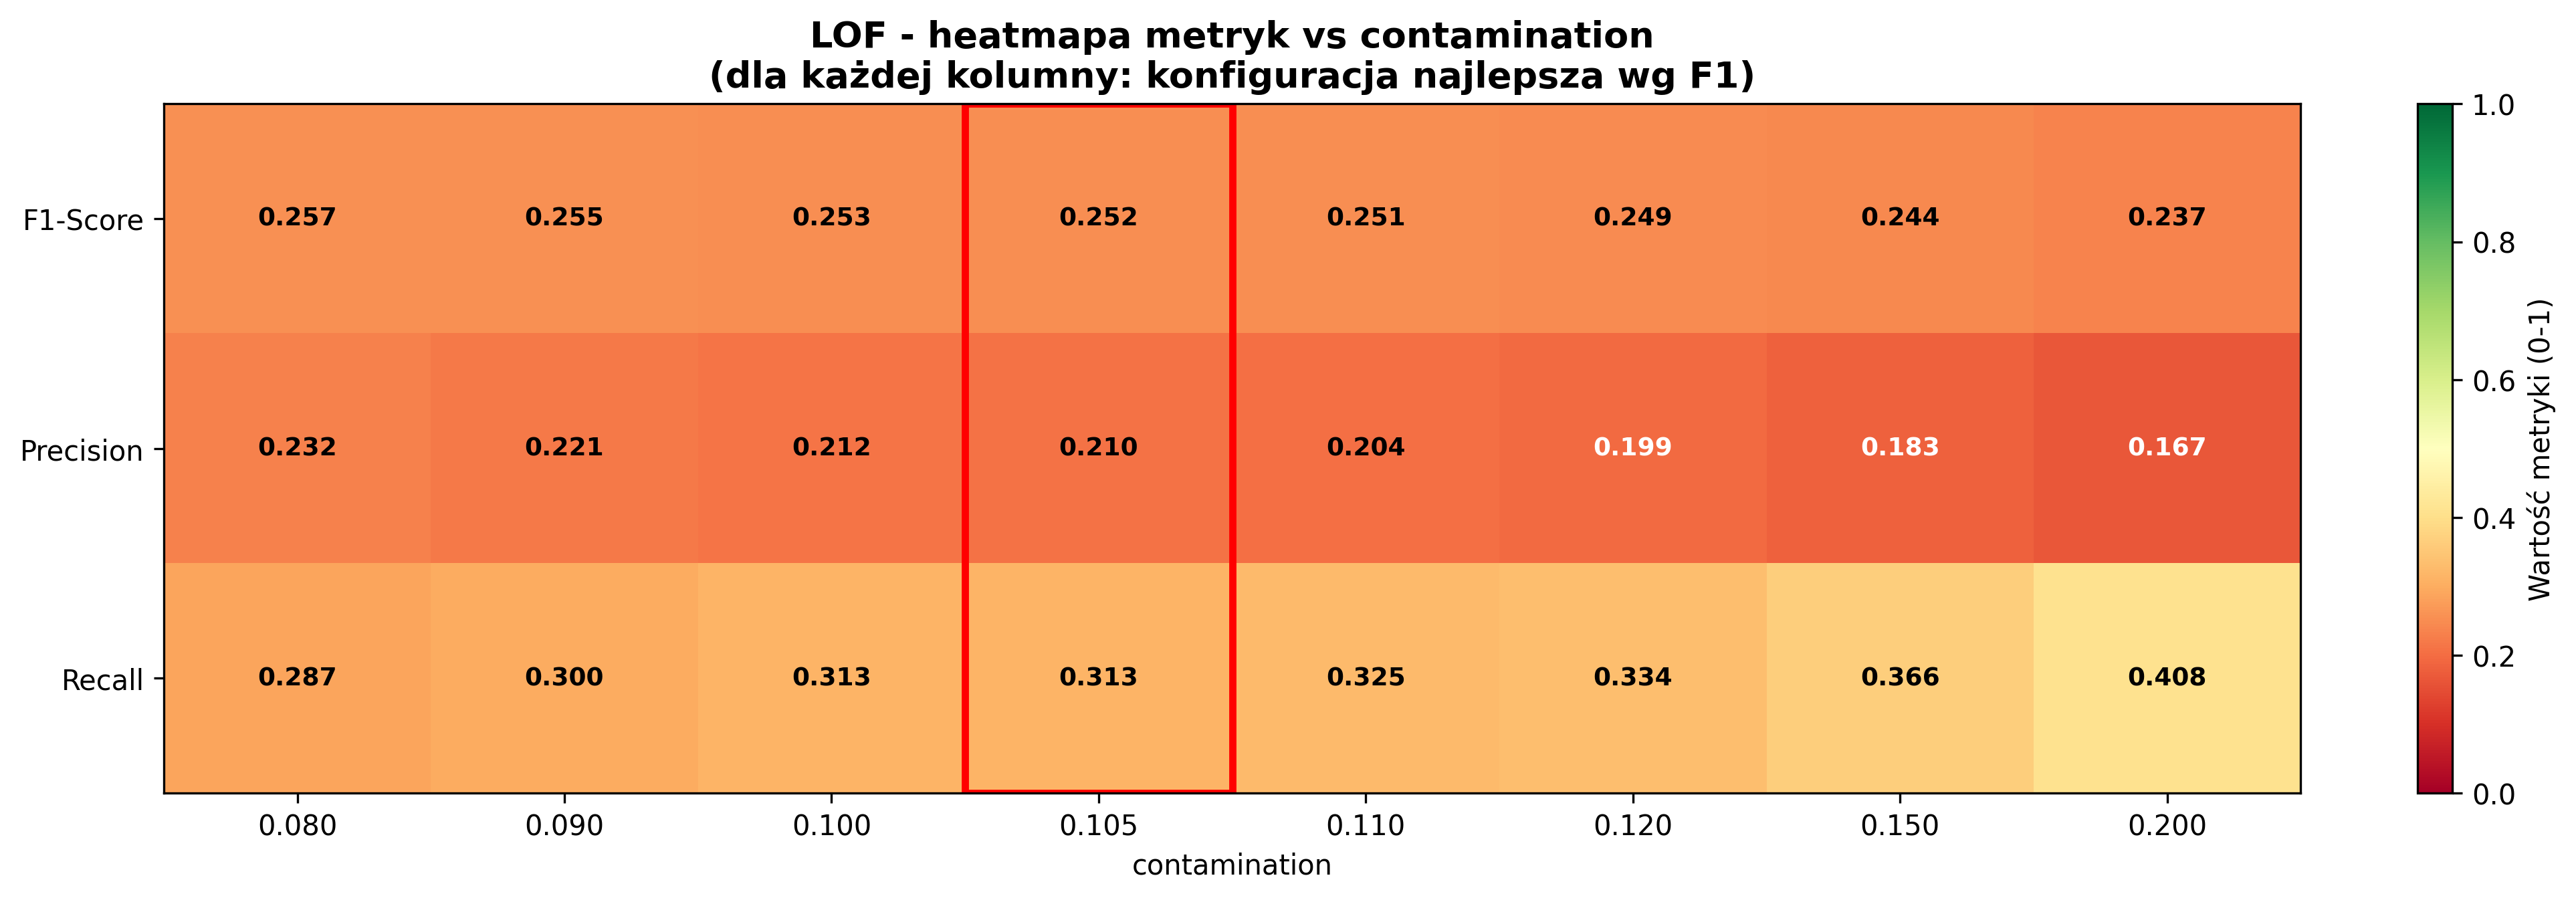
\includegraphics[width=0.9\textwidth]{fig_03b_lof_heatmap_v3.png}
		\caption{Macierz korelacji metryk z parametrem contamination(WIP) w algorytmie Local Outlier Factor}
		\label{fig:03b-lof-heatmap}
	\end{figure}
	Wyniki badania ukazane na rysunkach \ref{fig:03b-lof-params} i \ref{fig:03b-lof-heatmap}, pokazały, że większa liczba najbliższych sąsiadów $k$ negatywnie wpływa na mierzone miary, takie jak F1-Score, czy czułość, pomimo wzrostu precyzji, która nie kompensowała w wystarczający sposób spadków w drugiej mierze, co przekłada się na zmniejszający się F1. Dla małych $k$ modele zatrzymują swój lokalny charakter, gdyż zostaje w obszarze najbliższych sąsiadów, podczas gdy zwiększenie daje szerszy obszar, w którym metoda traci zdolności do kontekstowej ewaluacji modelu, co powoduje gorsze wyniki. W tej metodzie, a w przeciwieństwie do poprzedniej, drugi parametr mierzony, czyli \textit{contamination}, okazał się znaczący dla doboru optymalnej konfiguracji. W opozycji do algorytmu Isolation Forest najlepsze wyniki dawały mniejsze wartości \textit{contamination}. Wartości na poziomie 0{,}15, a zwłaszcza największa badana wartość, czyli 0{,}2 nie dorównały mniejszym, pomimo znacząco lepszej czułości modelu, która sięgała poziomów powyżej 0{,}4. Mapa na rysunku \ref{fig:03b-lof-heatmap} pokazuje najlepsze wartości miar dla parametru \textit{contamination}, nie biorąc pod uwagę liczby sąsiadów. Najlepszą konfiguracją okazała się para  $k$ w wysokości 5 i \textit{contamination} na poziomie 0{,}08, osiągając F1 na poziomie 0{,}2569, precyzją równą 0{,}2323 i czułość w wysokości 0{,}2874.
	
	\subsection{One-Class SVM}
	One-Class SVM jest algorytmem działającym poprzez określenie powierzchni, która oddziela dane normalne od tych oznaczonych jako anomalie w nowej przestrzeni cech. W ramach badań mierzono parametr $nu$, który definiuje dwie rzeczy, górną granicę ułamka błędów treningowych, a także dolną granicę frakcji wektorów nośnych. Jest to metoda generująca ogromne koszty obliczeniowe w porównaniu do reszty z klasy metod uczenia maszynowego, dlatego model ten trenowano na próbce 20000 danych. W dodatku do nauki wykorzystano tylko jądro liniowe, które było jedyną opcją wykonalną dla używanej platformy dla tej skali danych.
	\begin{figure}%[H]
		\centering
		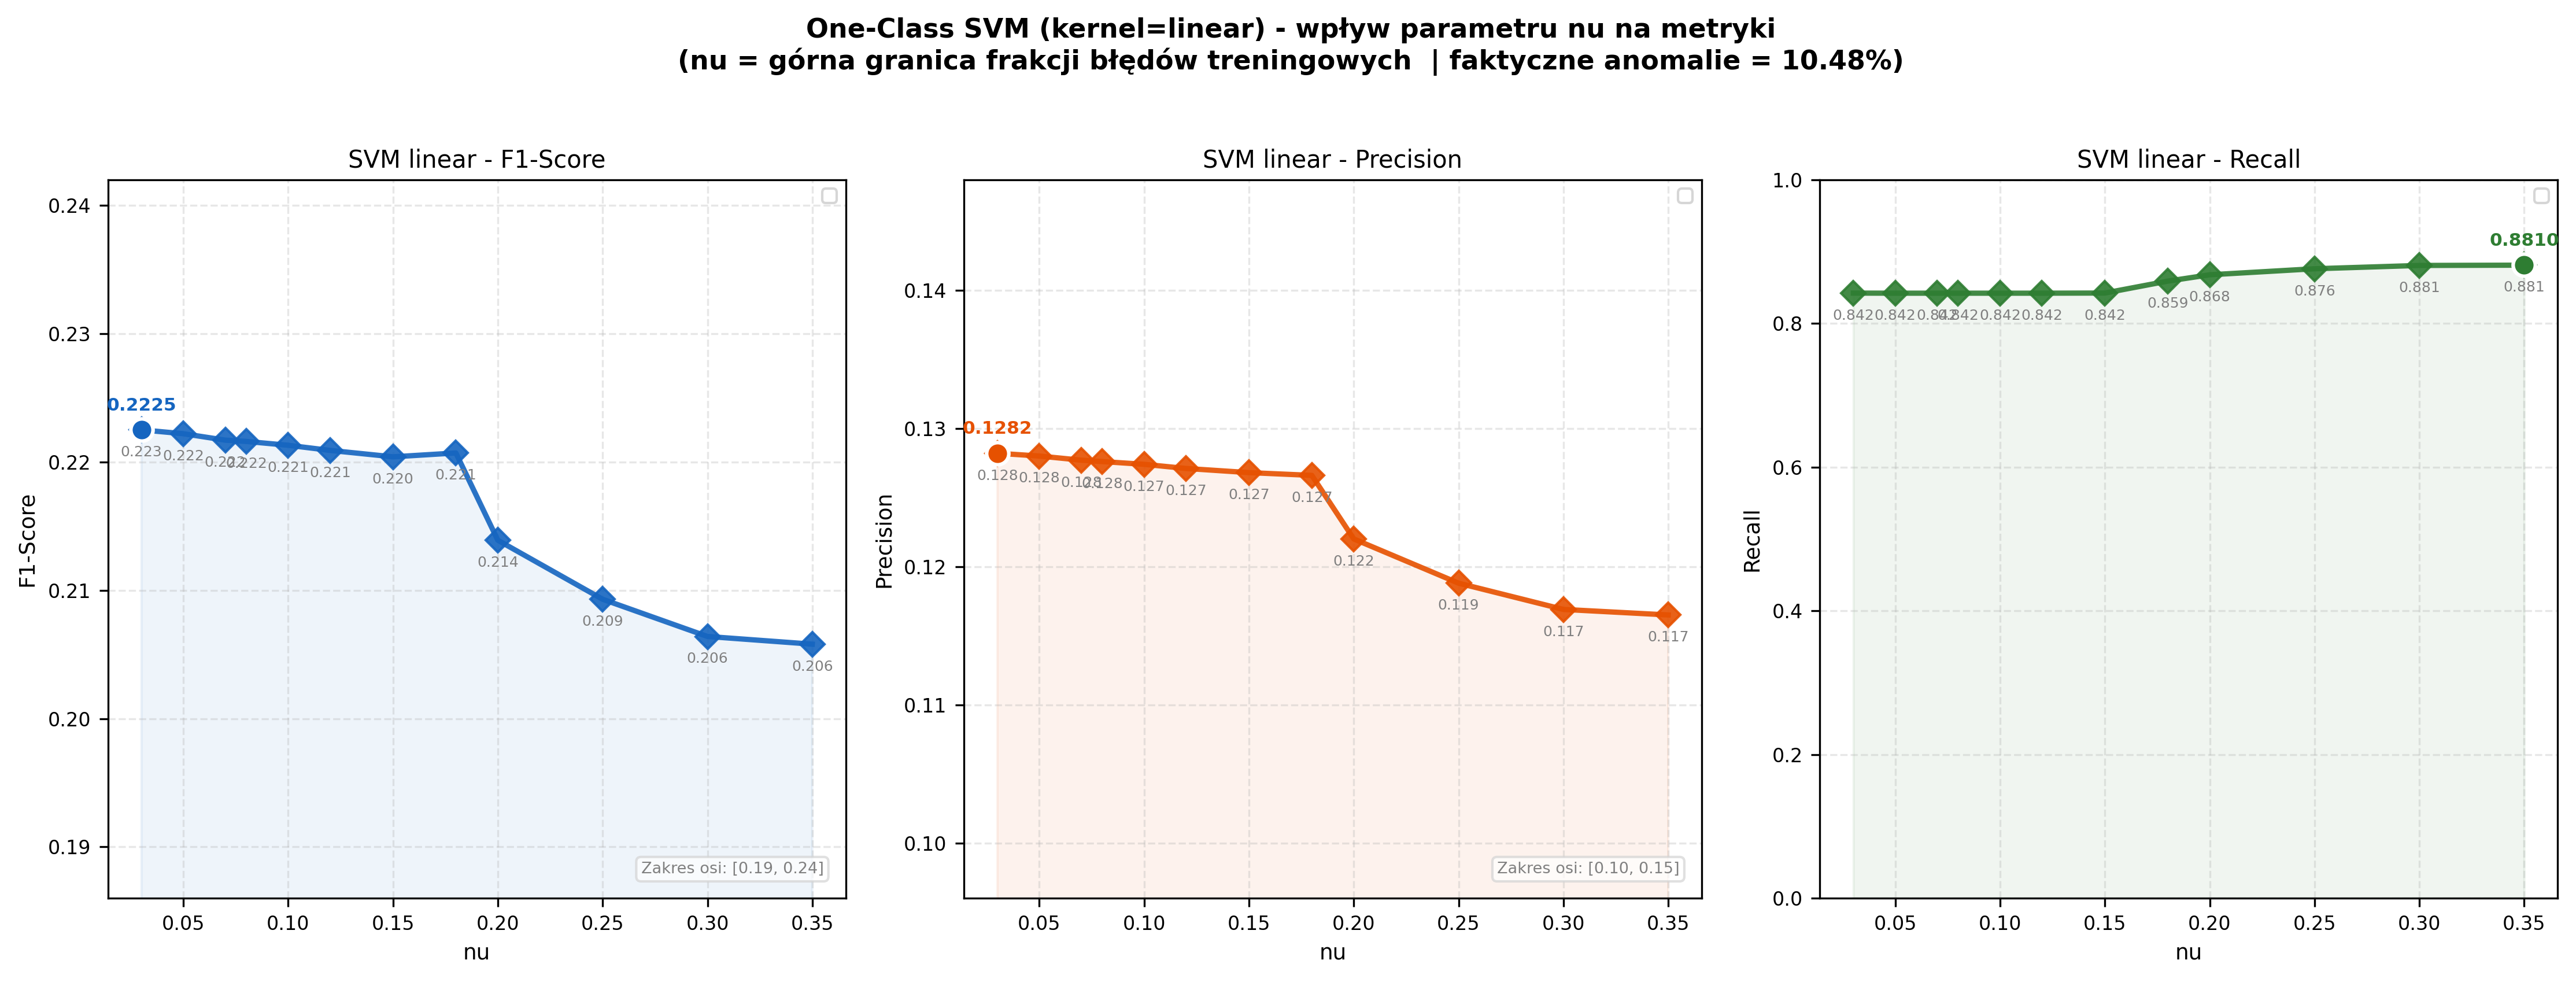
\includegraphics[width=0.9\textwidth]{fig_03b_svm_params_v4.png}
		\caption{Wpływ górnej granicy błędu na metryki decyzji w algorytmie One-Class SVM}
		\label{fig:03b-svm-mod-params}
	\end{figure}
	Rysunek \ref{fig:03b-svm-mod-params} przedstawia wynik ewaluacji tej metody. Ujawnia ona charakter wyników podobny do metod statystycznych, niska na tle konkurencji precyzja, lecz wyróżniająca się czułość modelu, trzymająca się powyżej poziomu 0{,}8. Metoda daje najlepsze wyniki dla najmniejszej wartości parametru $\nu$\,=\,0{,}05. Wraz ze wzrostem $\nu$ model jest mniej restrykcyjny, przez co powstaje więcej fałszywych alarmów, obniżając precyzję jeszcze niżej. Dlatego najlepsze wynika najbardziej surowa konfiguracja testowana, która osiągnęła F1-Score na poziomie 0{,}2225, przy precyzji równej 0{,}1282 i czułości 0{,}881.
	
	\subsection{K-Means}
	Metoda K-Means, zwana też algorytmem klastrowym lub centroidowym, jest metodą, która działa poprzez pogrupowanie danych w klastry, a za anomalie klasyfikuje próbki oddalone od najbliższego centroidu o odległość przekraczającą percentyl rozkładu odległości w zbiorze do trenowania. Parametrami testowanymi dla tej metody były ilość klastrów i wspomniany percentyl odległości.
	\begin{figure}%[H]
		\centering
		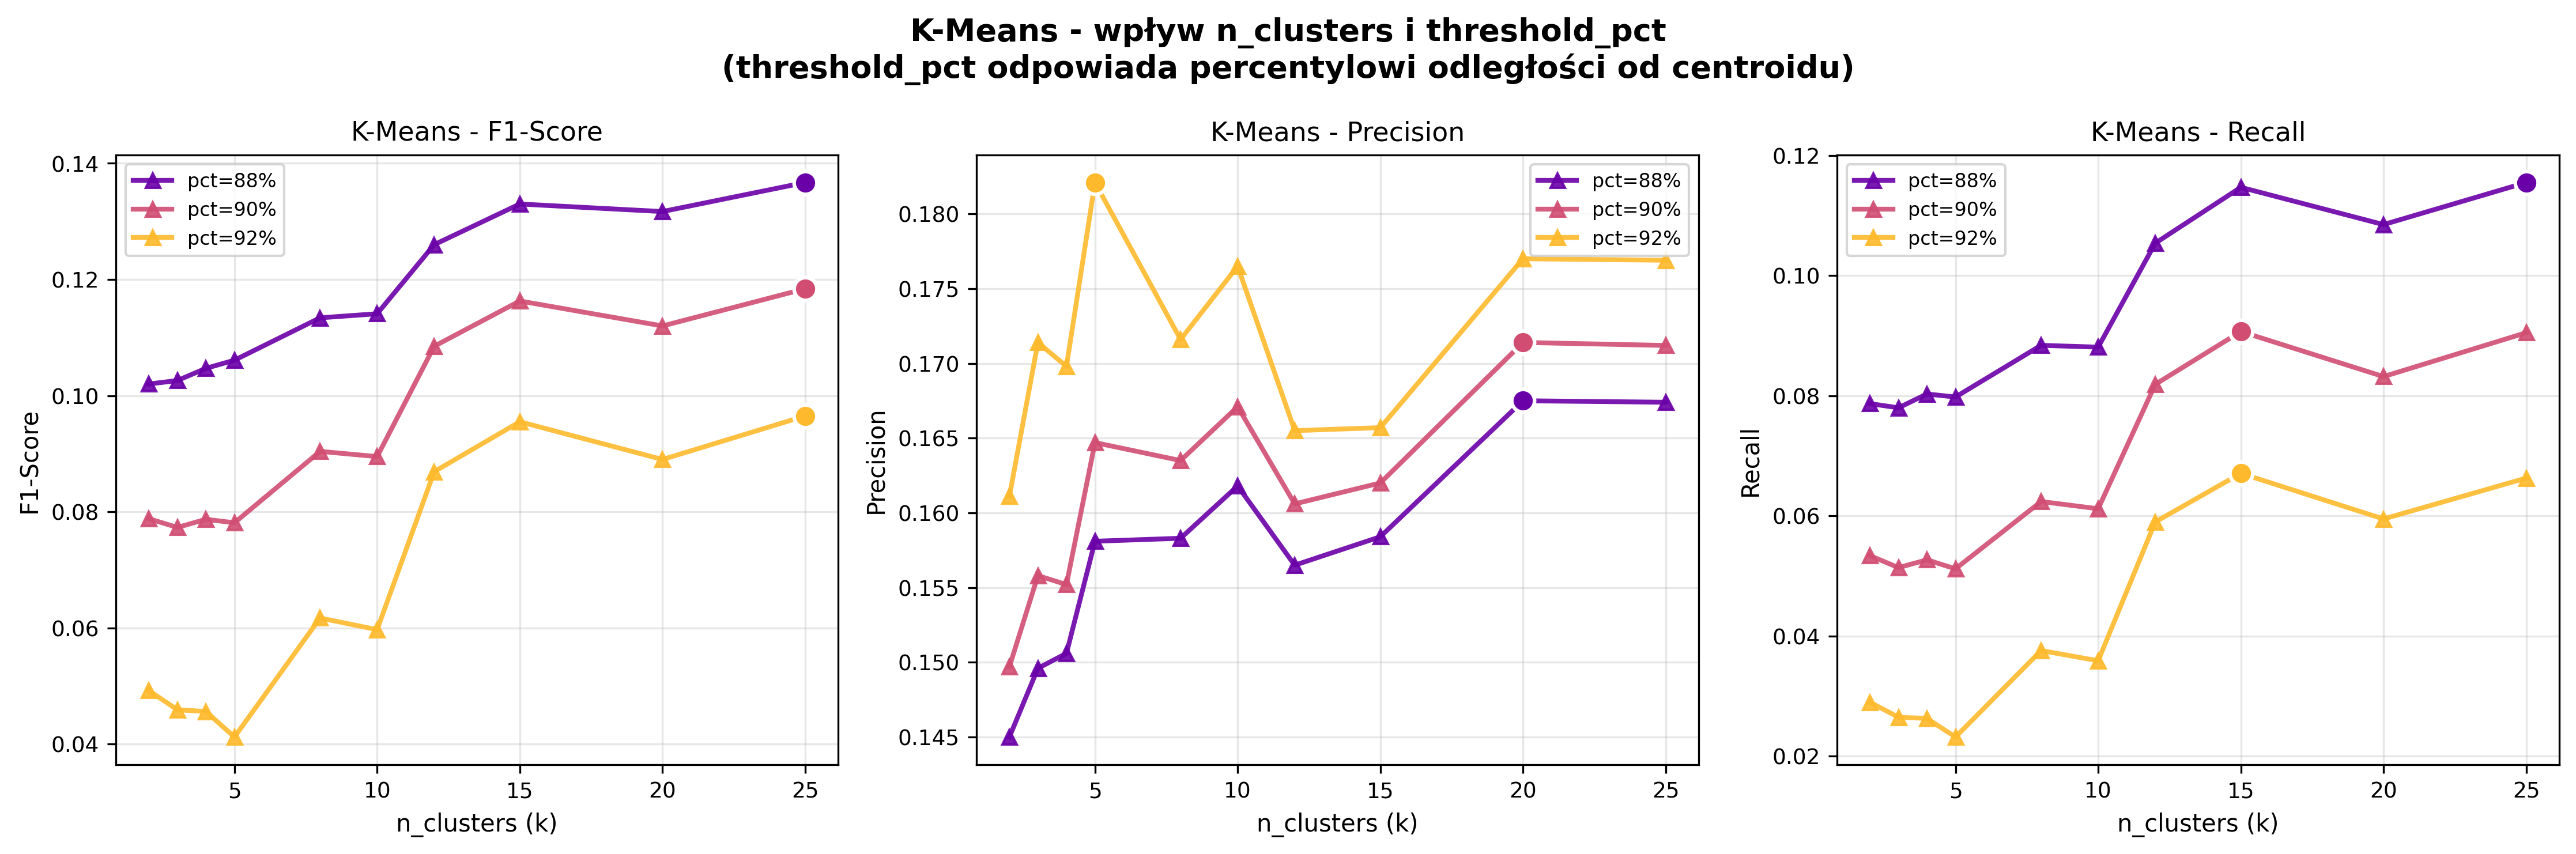
\includegraphics[width=0.9\textwidth]{fig_03b_kmeans_params_v2.png}
		\caption{Wpływ liczby klastrów na metryki detekcji w algorytmie K-Means}
		\label{fig:03b-kmeans-params}
	\end{figure}
	
	\begin{figure}%[H]
		\centering
		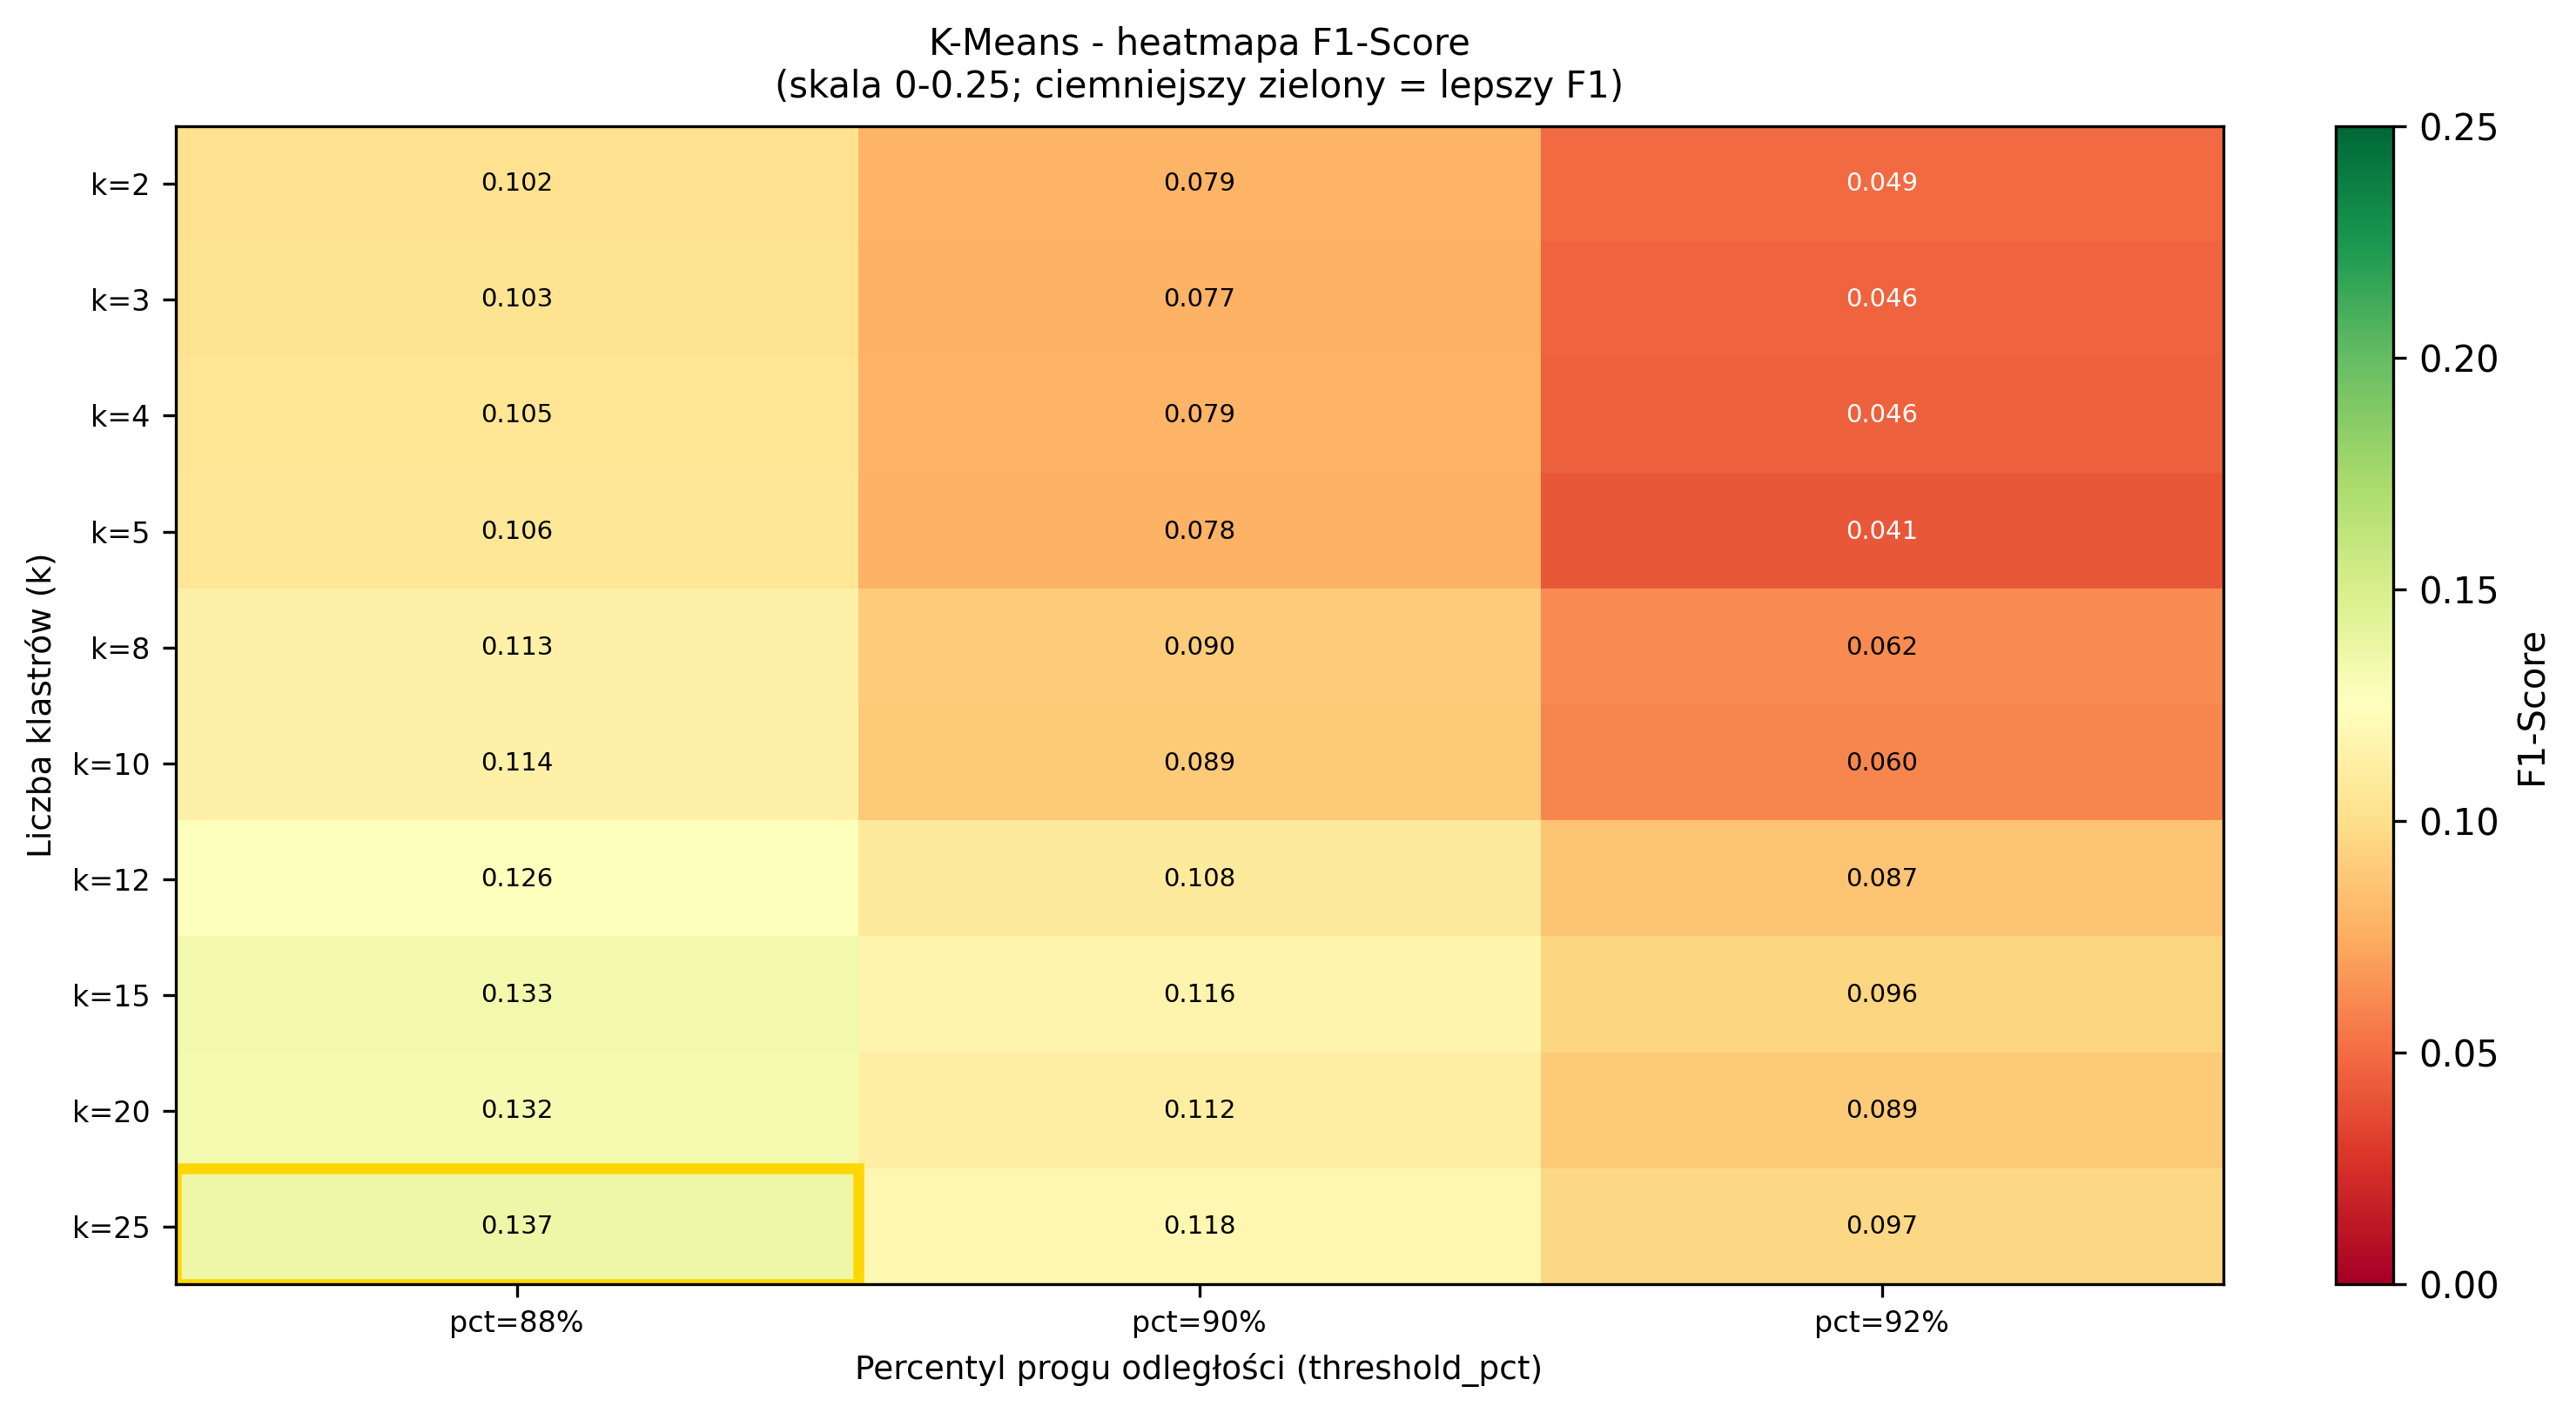
\includegraphics[width=0.9\textwidth]{fig_03b_kmeans_heatmap_v4.png}
		\caption{Macierz korelacji metryk z liczbą klastrów w algorytmie K-Means}
		\label{fig:03b-kmeans-heatmap}
	\end{figure}
	Wyniki, ukazane na rysunkach \ref{fig:03b-kmeans-params} i \ref{fig:03b-kmeans-heatmap}, okazały się najsłabsze w całym badaniu, dla najlepszej konfiguracji F1 wyniosło tylko 0{,}1367, które zostało osiągnięte dla największej sprawdzanej ilości klastrów, czyli 25. Główną przyczyną jest natura danych w badaniach. Technika klastrowania nie sprawdza się w wielokanałowej telemetrii, gdyż same dane nie są skupiskami wokół środkowej wartości, lecz szeregiem zależnym od kontekstu czasowego. Algorytm nie potrafi rozróżnić subtelnych zmian od naturalnego rozkładu próbek między klastrami. Patrząc na wyniki można stwierdzić, że zwiększenie percentyla odległości ma negatywny wpływ na wyniki. Ciekawym przypadkiem jest wysoka precyzja dla wysokiego progu odległości, która oznacza, że anomalie wykryte przez model okazały się prawdziwe, lecz z powodu małej czułości można uznać, że stanowiły one mały procent z wszystkich danych.
	
	\subsection{Podsumowanie wyników metod uczenia maszynowego}
	
	\begin{figure}%[H]
		\centering
		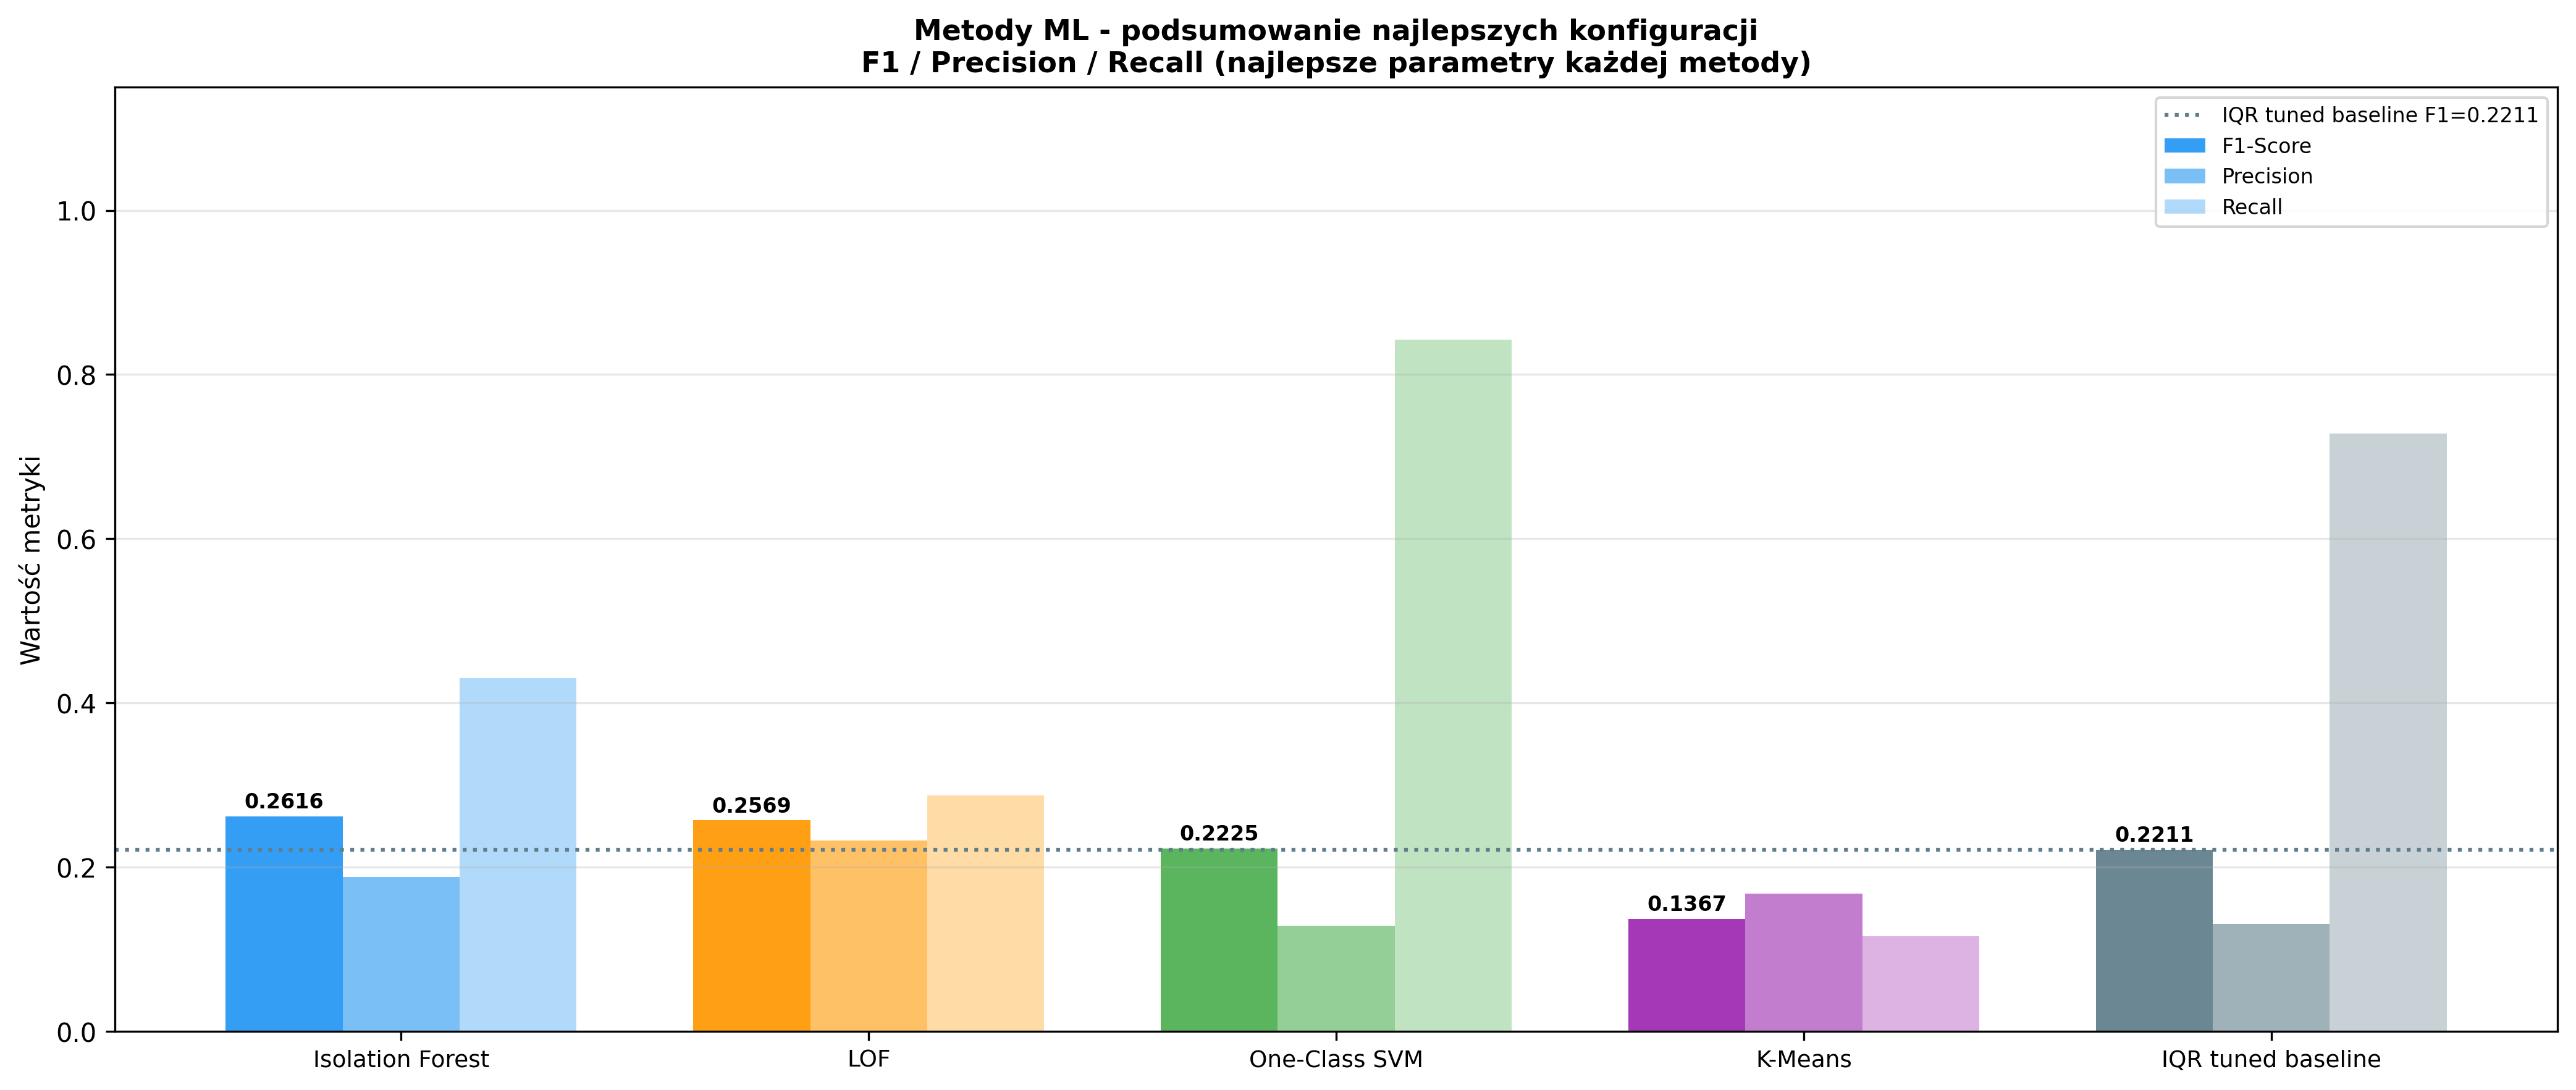
\includegraphics[width=0.9\textwidth]{fig_03b_summary_comparison.png}
		\caption{Porównanie metryk uzyskanych przez metody uczenia maszynowego z pierwszym progiem}
		\label{fig:03b-summary}
	\end{figure}
	Rysunek \ref{fig:03b-summary} zestawie najlepsze konfiguracje wszystkich wyników dla metod uczenia maszynowego. Najlepszą metodą okazał się algorytm Isolation Forest, który osiągnął F1-Score na poziomie 0{,}2611. Algorytm Local Outlier Factor miał niewiele gorszy wynik, gdyż osiągnął 0{,}2569, pomimo faktu, że precyzja była wyższa niż w przypadku IF, ale gorsza czułość ma większy wpływ na nieznacznie niższą miarę F1. Metoda One-Class SVM jest kolejną, która osiągnęła wynik lepszy od punktu odniesienia, ale nieznacznie, bo o raptem 0{,}001. Z kolei metoda K-Means nie uzyskał wymaganej skuteczności, gdyż jest nieodpowiednia do szeregów czasowych. Analizując wyniki wszystkich metod uczenia maszynowego można zauważyć, że osiągają one wszystkie lepszą precyzję niż algorytmy statystyczne, co ma duży wpływ na poprawę, natomiast poza SVM czułość metod uczenia maszynowego była wyraźnie niższa. Jest to wynik wielowymiarowej analizy cech, która lepiej nadaje się do analizy tego typu danych. 
	
	\section{Wyniki metod głębokiego uczenia i krzywe uczenia}
	Najbardziej zaawansowane metody testowane w ramach badań to są metody głębokiego uczenia oparte na technice autoenkodera, która kompresuje dane, by potem dzięki treningowi je odtworzyć. W tej części przetestowano cztery metody, oparte na trzech typach sieci neuronowych. Główną miarą determinującą klasyfikację danej jest błąd w rekonstrukcji danych zbioru treningowego, ustalony na 90 percentyl. Wejściem modelu do ewaluacji, jest ten sam wektor cech okna kroczącego, który działał dla poprzednich metod. Aby uniknąć przeuczenia sieci, zastosowano mechanizm (\textit{early stopping}), który w momencie gdy dalsze epoki trenowania sieci nie dają odpowiednich rezultatów, przerywa naukę i uruchamia inną konfigurację. 
	
	\subsection{Dense Autoencoder}
	Autoenkoder oparty jest na technice głębokiej sieci neuronowej, która składa się z warstw, które są w pełni połączone ze sobą, każda część poprzedzająca wysyła dane do kolejnego węzła, który zbiera informacje ze wszystkich we wcześniejszej. Próbki z cechami modelu okna kroczącego są kompresowane do tzw. wąskiego gardła (\textit{bottleneck}), a potem dekoder dokonuje odtworzenia pierwotnego stanu. Jeżeli próbka będzie posiadała błąd rekonstrukcji powyżej wartości progowej, jest uznawana za anomalię. 
	
	\begin{figure}%[H]
		\centering
		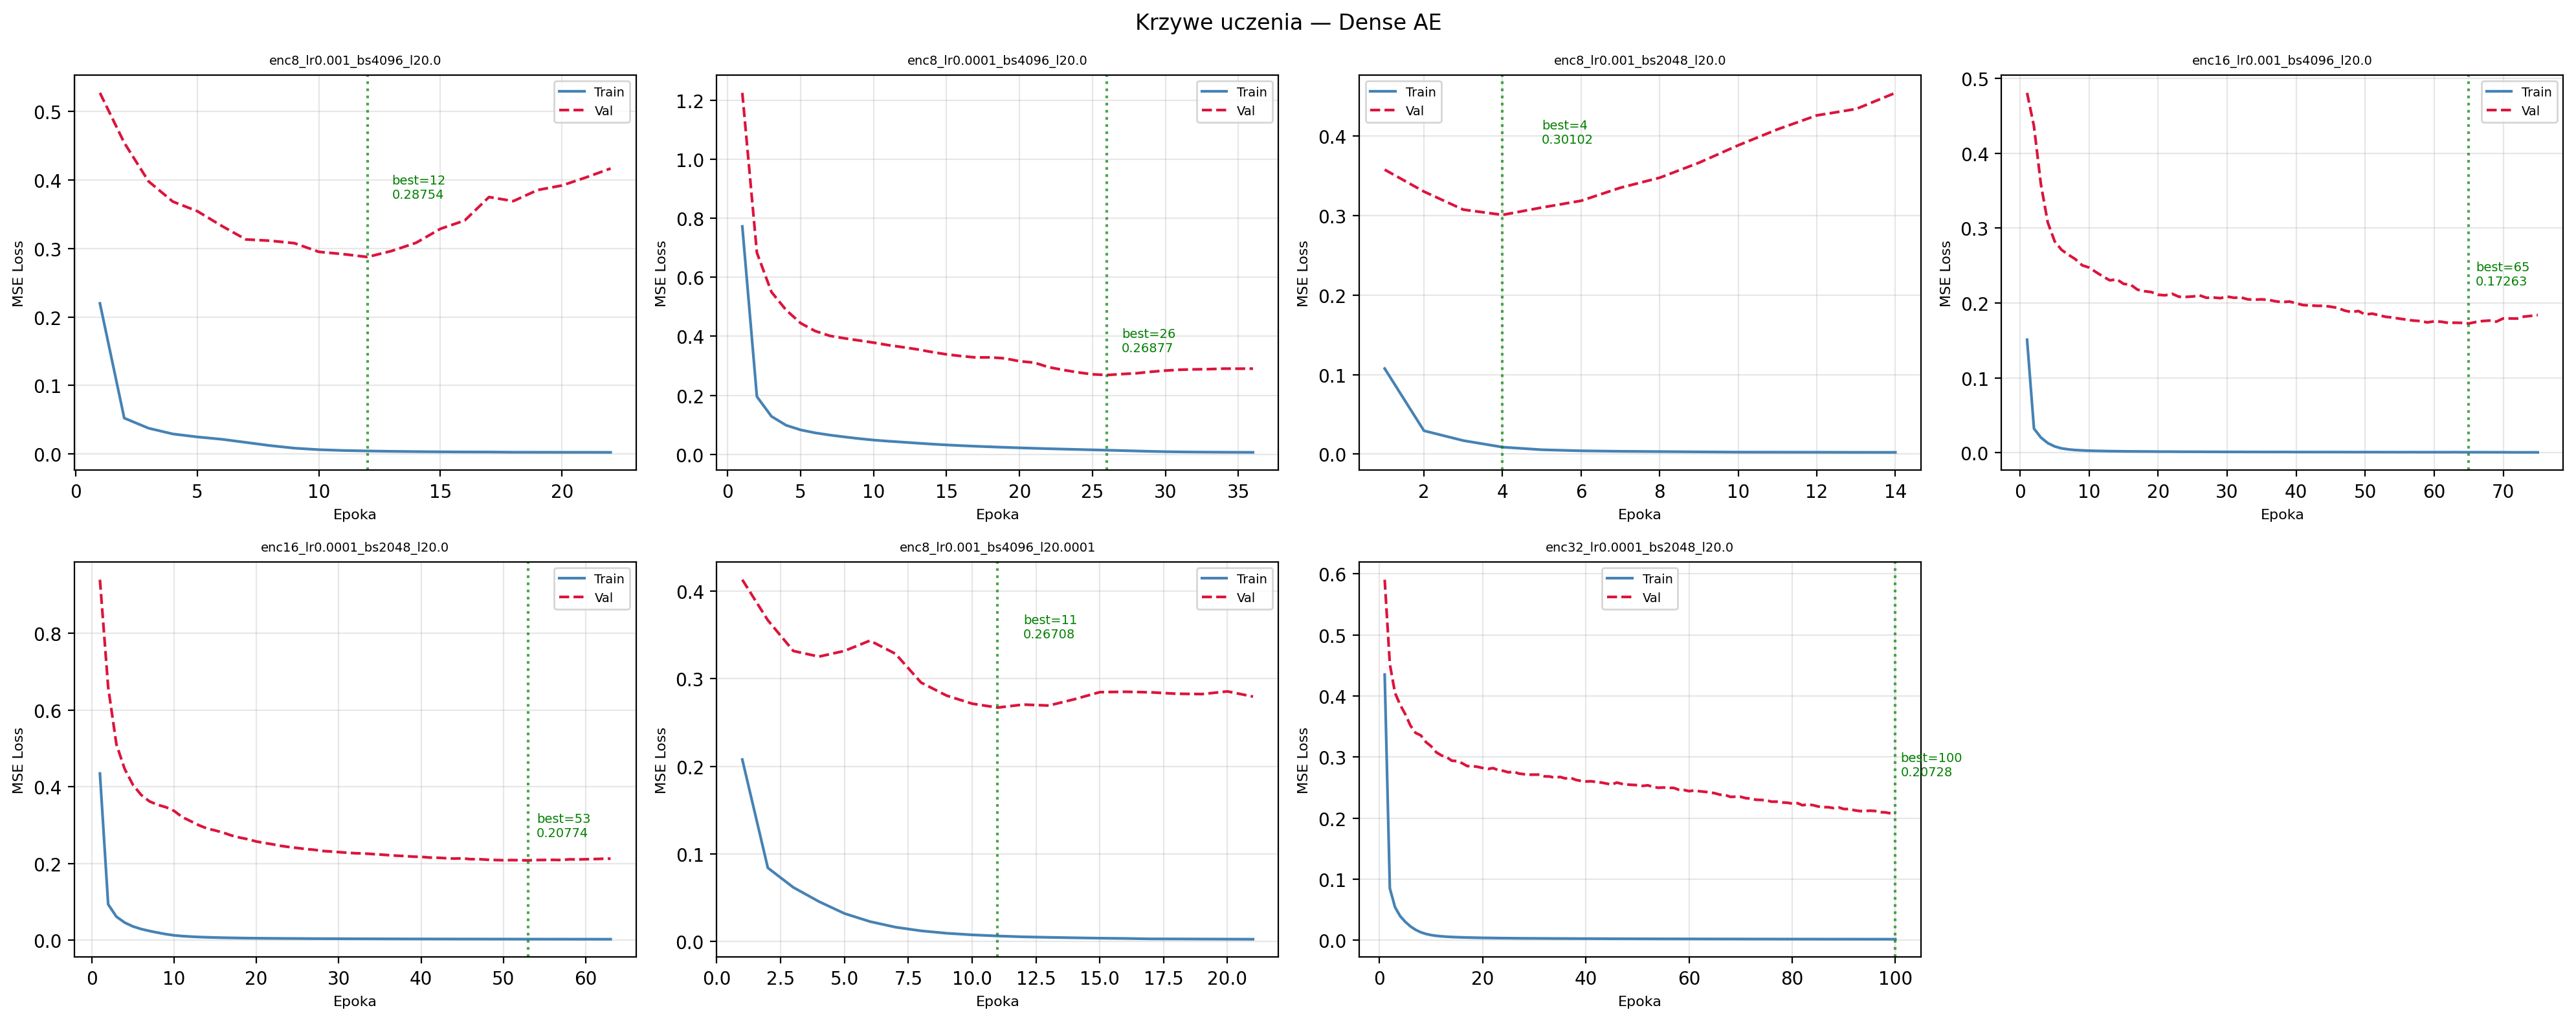
\includegraphics[width=0.9\textwidth]{fig_04b_curves_Dense_AE.png}
		\caption{Krzywe uczenia modelu sieci neuronowej w metodzie gęstej sieci neuronowej}
		\label{fig:04b-curves-dense}
	\end{figure}
	
	Rysunek \ref{fig:04b-curves-dense} przedstawia krzywe uczenia modelu autoenkodera opartego na architekturze gęstej. Każdy z wykresów przedstawia krzywe straty w treningu i walidacji i ich wartości z każdą kolejną epoką, dla różnych parametrów, a zieloną linią oznaczone zostały epoki, w których uzyskaną najniższą stratę walidacji wyrażoną przez miarę MSE (\textit{Mean Square Error}),. Każdy z modeli w tej architekturze posiada rozmiar warstwy kodującej (\textit{enc}). Mniejsza wartość powoduje silniejszą kompresję danych. Następnie występuje współczynnik uczenia (\textit{lr}) który opisuję rozmiar kroku, jaki wykonuje optymalizator podczas dostosowywania wag. Wielkość paczki próbek potrzebnej do aktualizacji wag modelu (\textit{batch size}) jest następny, a na koniec jest współczynnik regularyzacji (\textit{l2}), który ma za zadania ograniczanie zbyt dużych wartości wag, w celu zapobieganiu przeuczenia. Jeżeli widnieje wartość 0{,}0, oznacza ona brak tego ograniczenia. We wszystkich konfiguracjach badanych strata treningowa znacznie opada dla pierwszych epok do wartości bliskich zeru, natomiast strata walidacyjna cały czas pozostaje na poziomie od  0{,}17 do 0{,}30 w przypadku minimum. Po osiągnięciu wspomnianej wartości minimalnej, strata waldacyjna wykazuje także tendencję wzrostową w dalszych epokach. Jest to skutek przeuczenia sieci. Nieregulowana architektura pamięta dane treningowe zamiast uczyć się wzorców ogólnych sygnału. 
	
	\subsection{Dense Autoencoder z mechanizmem Dropout}
	
	Następna metoda, od poprzedniej miała tylko jedną różnicę. Jest nią dodanie warstwy Dropout. Jest to technika regulacji, która w trakcie wykonywania treningu dokonuje losowego wyłączania poszczególnych neuronów w warstwie. Ma to na celu zapobieganie koadaptacji neuronów i nałożenie przymusu nauki bardziej rozproszony reprezentacji. Mechanizm Dropout stosowany jest wyłącznie w warstwie kompresującej. 
	
	\begin{figure}%[H]
		\centering
		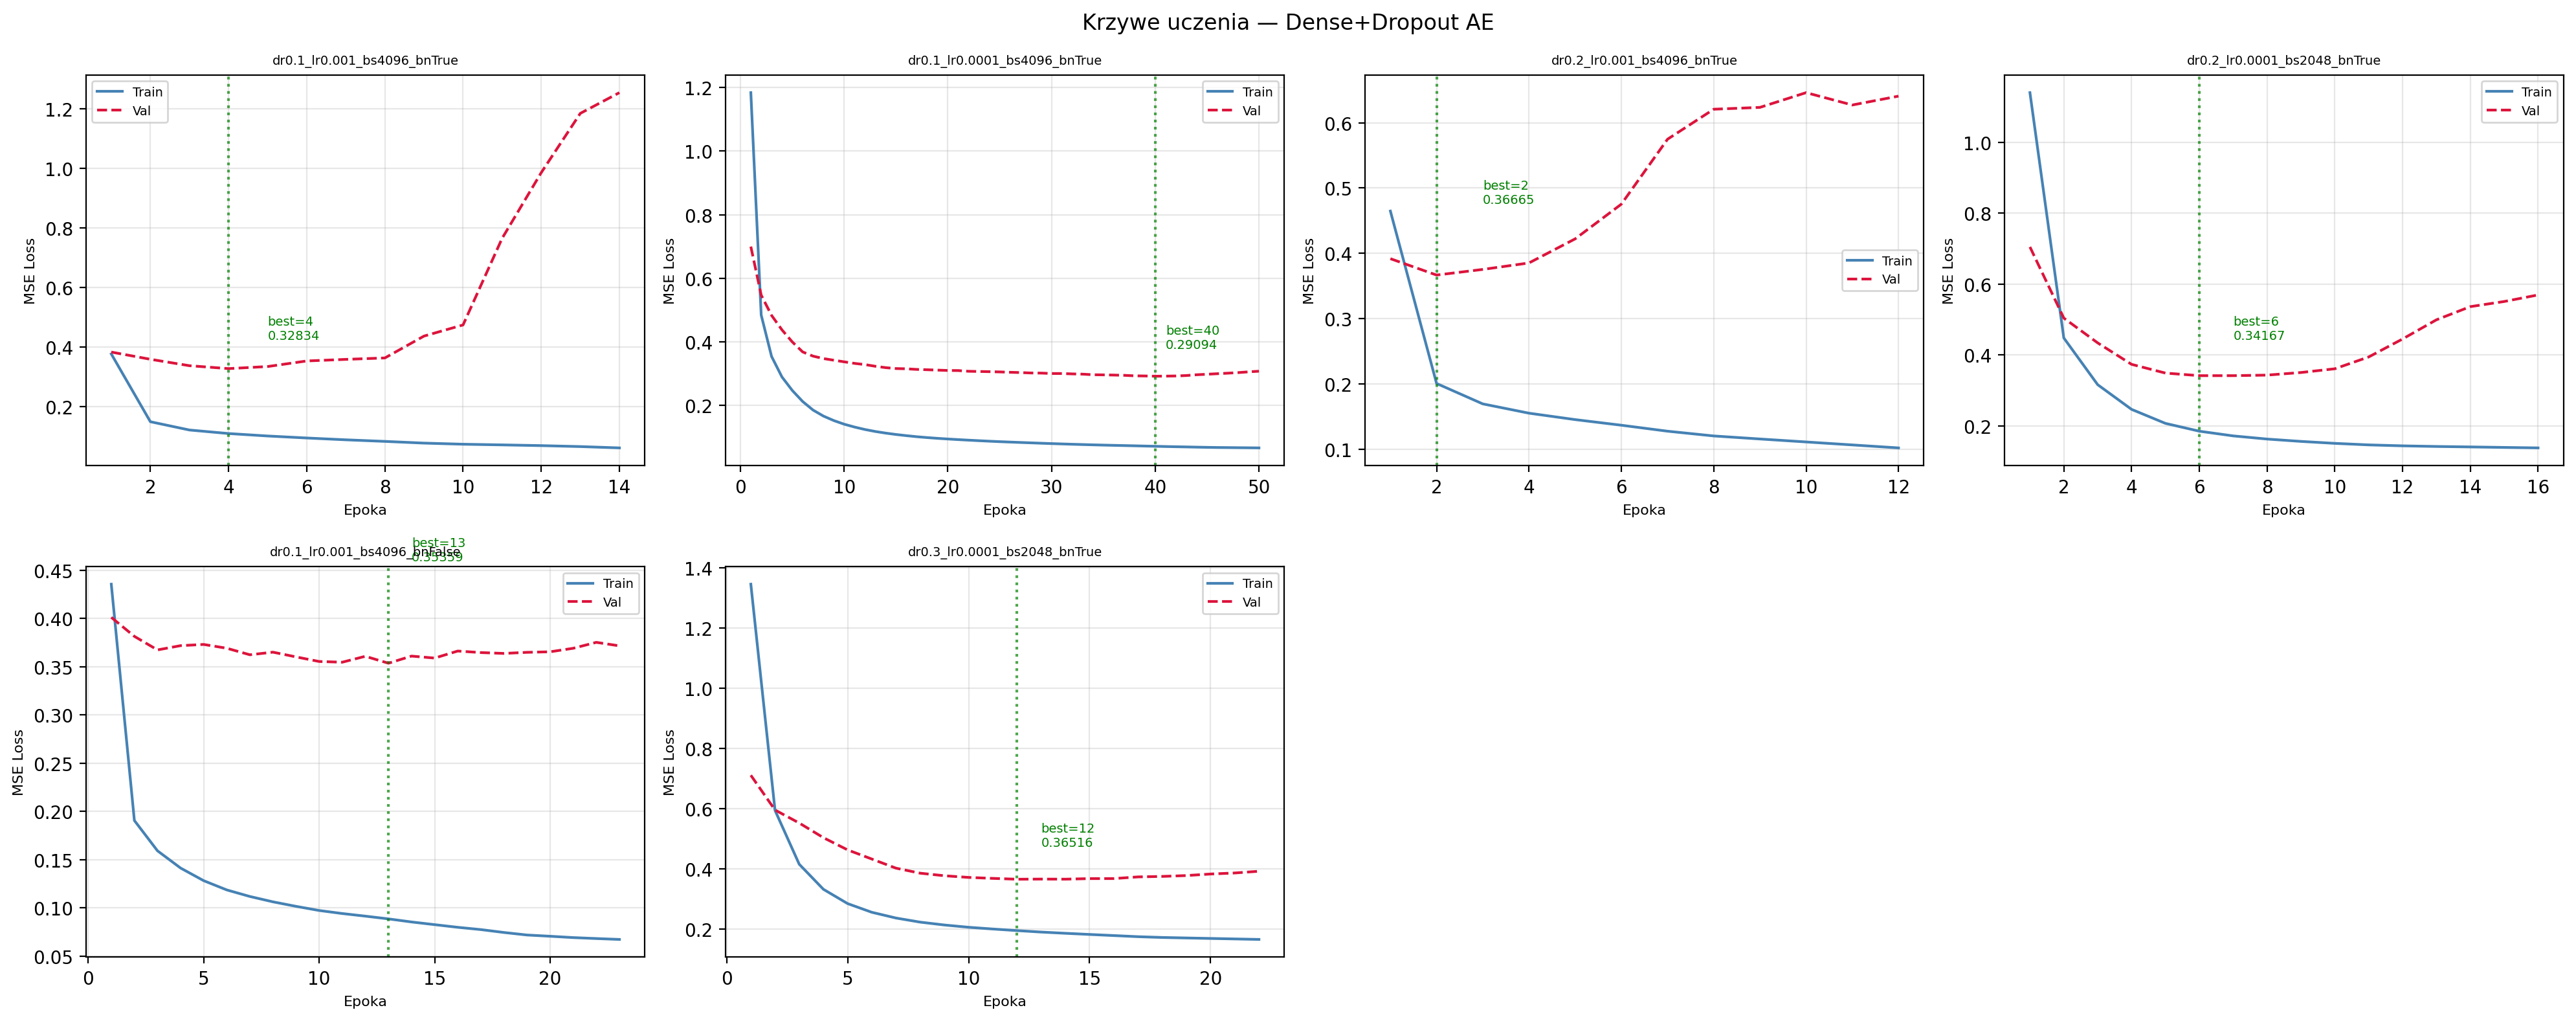
\includegraphics[width=0.9\textwidth]{fig_04b_curves_Dense+Dropout_AE.png}
		\caption{Krzywe uczenia modelu sieci neuronowej w metodzie gęstej sieci neuronowej z droputem}
		\label{fig:04b-curves-dense-dropout}
	\end{figure}
	
	Rysunek \ref{fig:04b-curves-dense-dropout} prezentuje krzywe uczenia modelu dla gęstej sieci z dropoutem. Zastosowano 2 inne parametry do oznaczenia poszczególnych modeli w porównaniu do zwykłej sieci gęstej. Pierwszy z nich (\textit{dr}) oznacza poziom dropoutu np. współczynnik 0{,}2 oznacza losowe wyłączanie 20 \%  neuronów w trakcie treningu. Ostatni parametr charakteryzujący konfigurację to normalizacja próbki (\textit{bnTrue / bnFalse}). Informuje o tym, czy paczka próbek była normalizowana, w celu stabilizacji procesu nauki sieci. Powoduje to stabilniejszy trening i niższą wartość funkcji straty.  Zauważyć można zwiększone straty walidacyjne MSE dla gęstej sieci z dropoutem, które potrafią być większe o 0{,}1, względem bez dropoutu. Najlepszą konfiguracją pod względem głównych miar okazała się być ta z dropoutem wynoszącym 20 \%, współczynnikiem uczenia 0.001, paczką 4096 próbek, z zastosowaną normalizacją. Osiągnęła po 12 epokach uczenia F1-Score na poziomie 0{,}3461, precyzję 0{,}2604 i czułość 0{,}5158, poprawiając wyniki uzyskane przez sieć bez dropoutu. Należy zaznaczyć, że trenowanie konfiguracji zakończyło się w ciągu zaledwie 2 epok, co dowodzi szybkiej zbieżności modelu przy tym zestawie parametrów.
	
	\subsection{CNN-1D Autoencoder}
	W tym eksperymencie wykorzystano architekturę konwolucyjnej sieci neuronowej z jednowymiarowymi warstwami, która w miejsce gęstych warstw posiada przesuwne filtry, które mają za zadanie nauczenie się lokalnych wzorców w cechach. CNN wychwytuje lokalne korelacje między elementami leżącymi obok siebie w wektorze wejściowym, w odróżnieniu od architektury gęstej, która globalnie analizuje wszystkie cechy. 
	
	\begin{figure}%[H]
		\centering
		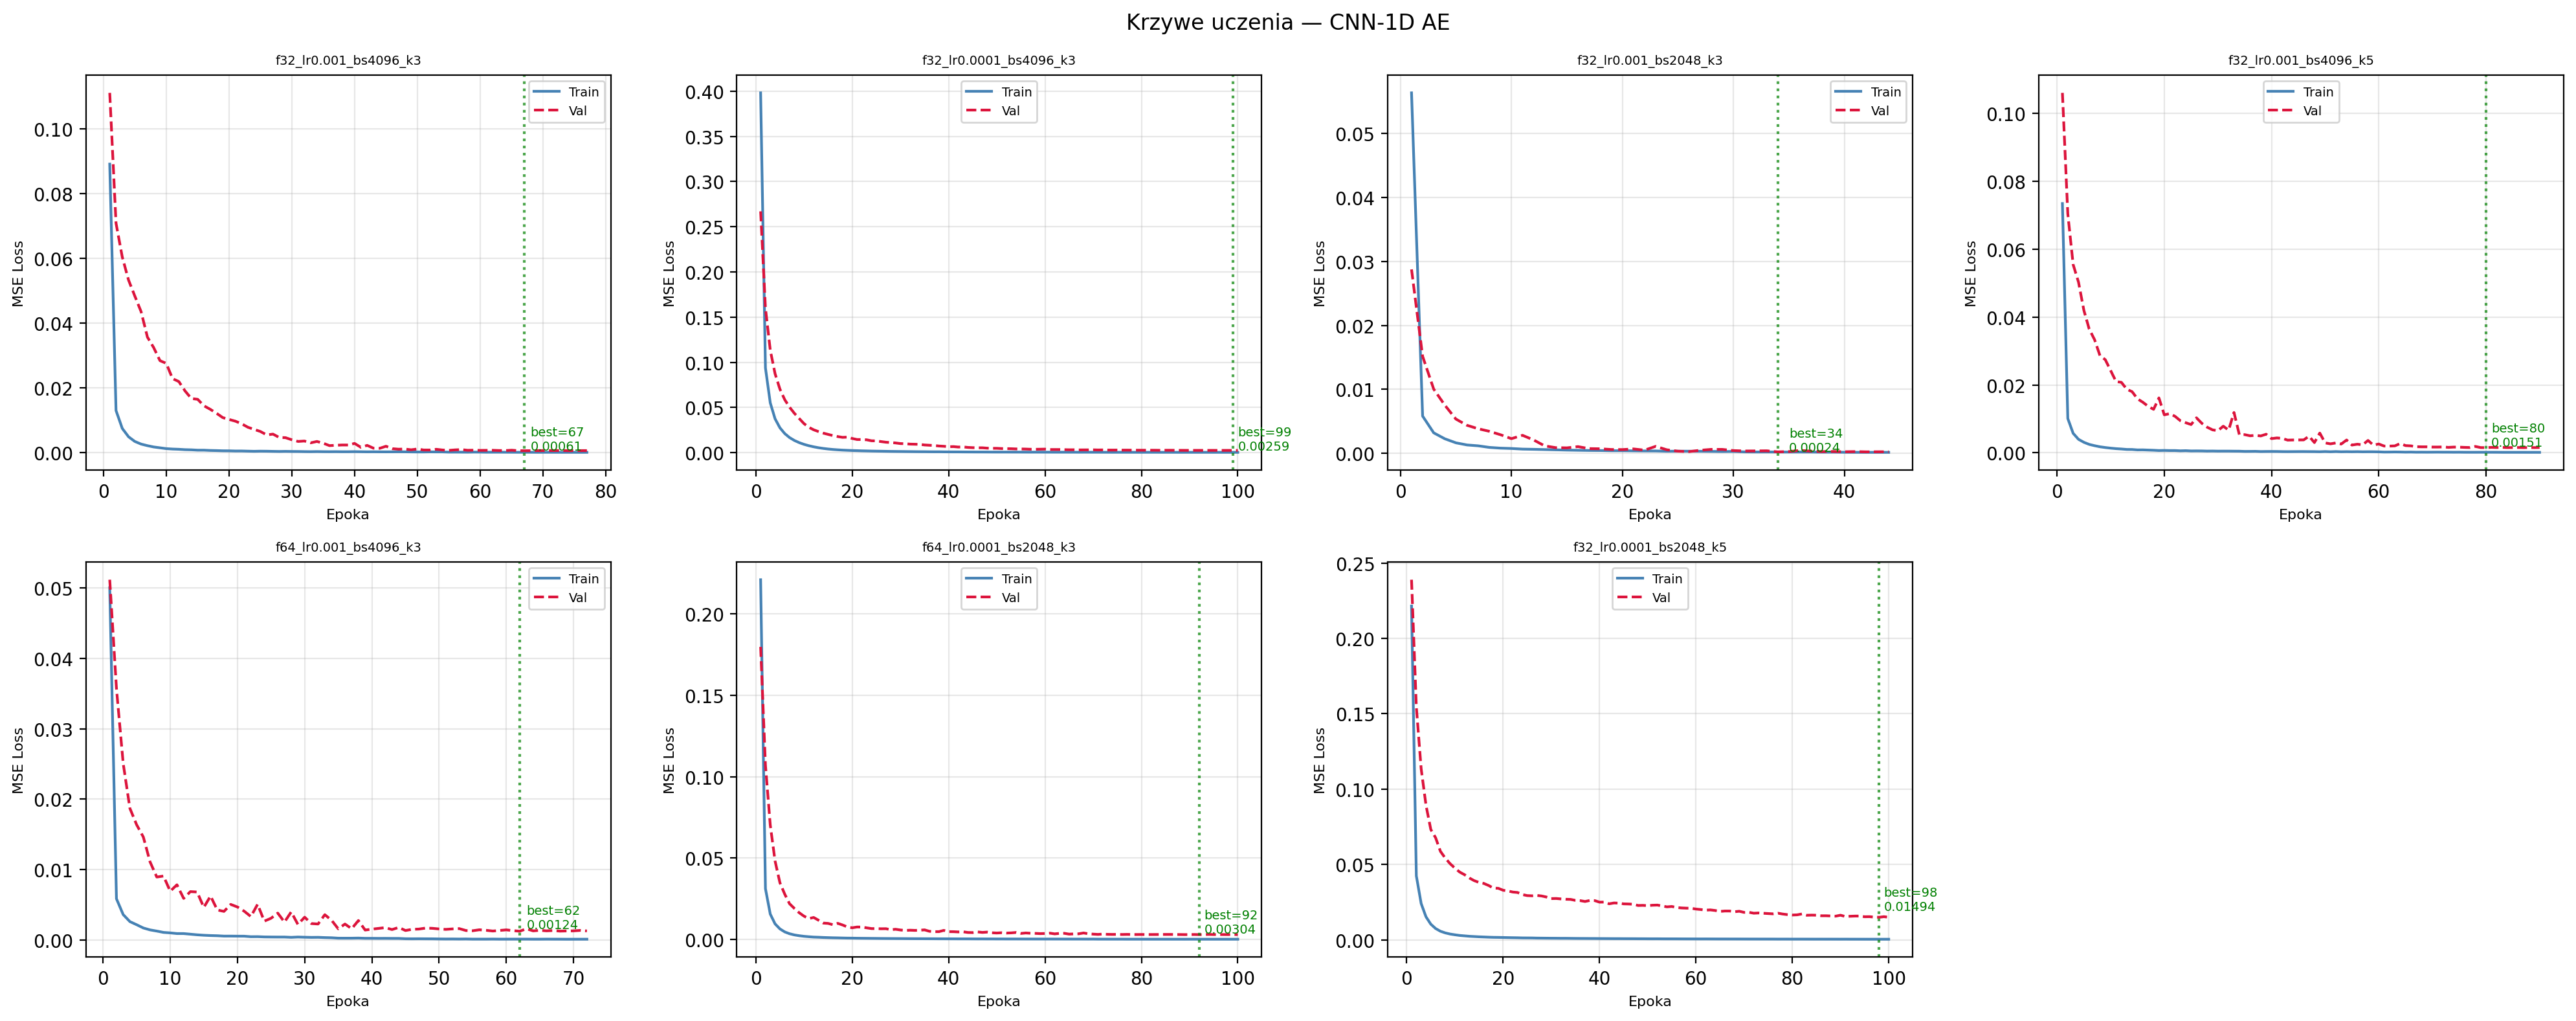
\includegraphics[width=0.9\textwidth]{fig_04b_curves_CNN-1D_AE.png}
		\caption{Krzywe uczenia modelu sieci neuronowej w metodzie konwolucyjnej sieci neuronowej}
		\label{fig:04b-curves-cnn1d}
	\end{figure}
	
	Rysunek \ref{fig:04b-curves-cnn1d} pokazuje różnice na krzywych straty względem gęstych sieci. Używa, tak jak pozostałe metody współczynnika uczenia i rozmiaru paczki, ale posiada też da charakterystyczne parametry. Pierwszy z nich (\textit{f}) oznacza ilość filtrów koewolucyjnych znajdujących się w pierwszej warstwie. Drugi paramet, osobliwy dla tej metody to rozmiar jądra konwolucji (\textit{k}). Wartość oznacza długość lokalnych fragmentów analizowanych przez warstwę konwolucyjną sieci.  Straty walidacyjne są zdecydowanie niższe, niż w poprzednich architekturach, gdyż sięgają wartości rzędu od 0{,}001 do 0{,}003, gdzie straty treningowe zbieżne są do wartości rzędu $10^(-4)$. Obie krzywe opadają równolegle, co nie miało miejsca w poprzednich metodach, gdyż oznacza brak znaków o przeuczeniu sieci. Długość treningu też jest znacznie dłuższa, bo sieć ta potrafi być trenowana przez co najmniej kilkadziesiąt epok, co trwa zdecydowanie dłużej niż w przypadku gęstych sieci. Najlepszą konfiguracją pod względem miar była ta z 32 filtrami, współczynnikiem uczenia 0{,}0001, paczką danych o rozmiarze 4096 i o rozmiarze jądra konwolucji 3 fragmentów. Osiągnęła F1-Score w wysokości 0{,}3284, precyzję 0{,}2396 i czułość na poziomie 0{,}5218. 
	
	\subsection{LSTM Autoencoder}
	
	LSTM oznacza Long Short-Term Memory i jest specjalnym rodzajem sieci neuronowej o architekturze rekurencyjnej. Autoenkoder oparty na tej technice modeluje zależności sekwencyjne w czasie, gdzie każda próbka jest analizowana w kontekście poprzednich, a stan ukryty sieci przechowuje krótkotrwałą pamięć. W warstwach kodujących i dekodujących także zastosowano dropout. Ze względu na znaczny koszt obliczeniowy trenowanie sieci przeprowadzono na ograniczonej próbce 200000 próbek. Dane zostały przekształcone do sekwencji 10 próbek w pamięci, które tworzyły sekwencje wejściowe do treningu autoenkodera LSTM. 
	
	\begin{figure}%[H]
		\centering
		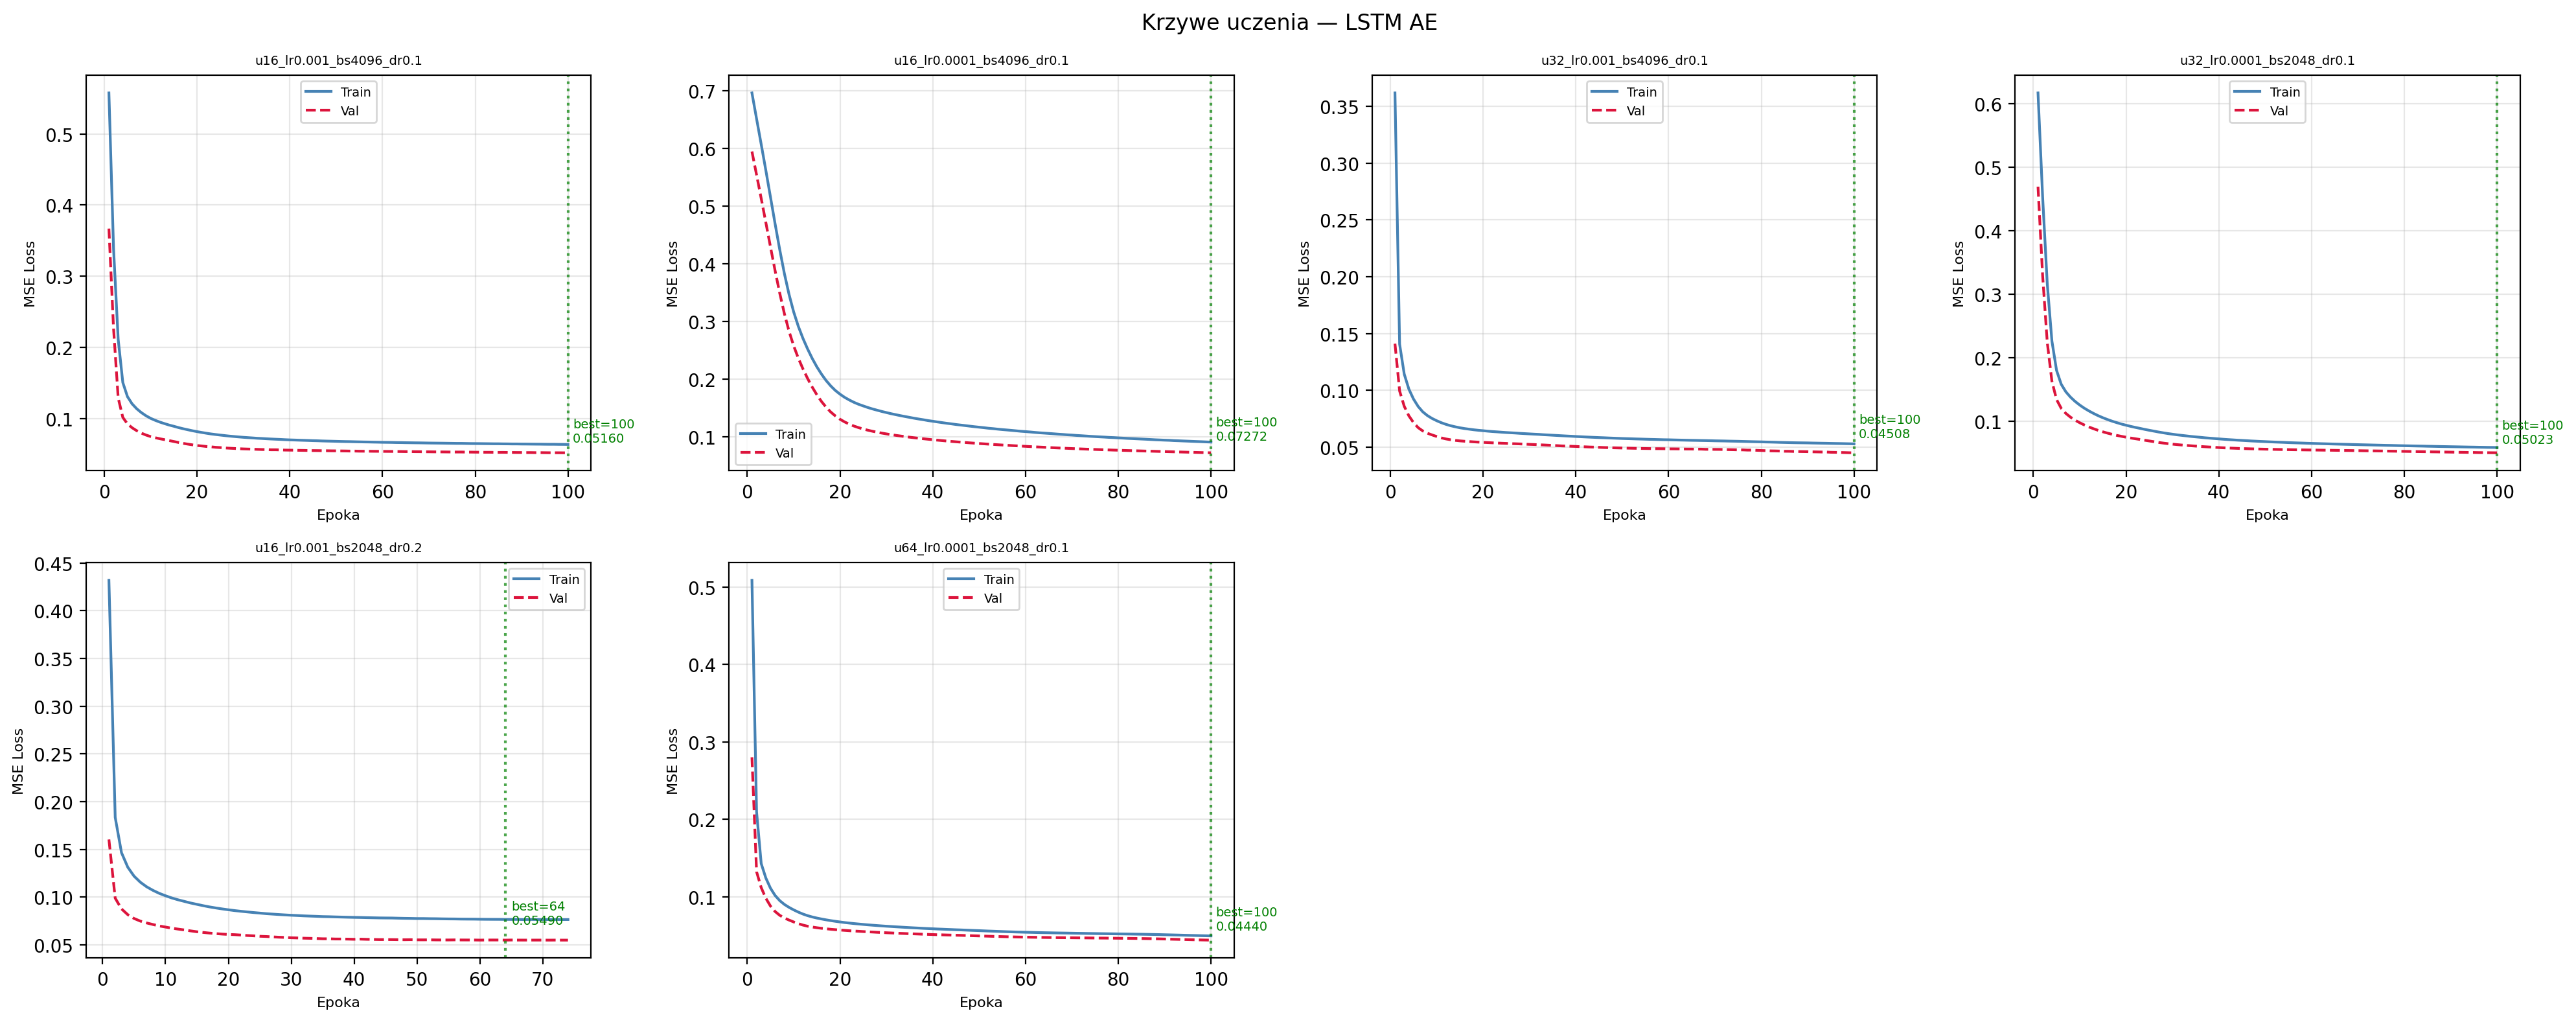
\includegraphics[width=0.9\textwidth]{fig_04b_curves_LSTM_AE.png}
		\caption{Krzywe uczenia modelu sieci neuronowej w metodzie rekurencyjnej sieci neuronowej}
		\label{fig:04b-curves-lstm}
	\end{figure}
	
	Rysunek \ref{fig:04b-curves-lstm} przedstawia wyniki krzywych uczenia z zaznaczonymi stratami i od razu narzuca się pierwszy wniosek. W porównaniu do architektury gęstej, obie krzywe przebiegają równolegle do siebie. Długość treningu też była duża, bo na 6 testowanych konfiguracji, aż 5 trenowało pełne 100 epok ustawione jako górny limit, ze względu na ograniczenia czasowe. Modele tej sieci posiadały tylko jeden charakterystyczny parametr, jednostki pamięci (\textit{u}), które oznaczają ilość komórek w warstwie rekurencyjnej, którą model wykorzystuje do nauki zależności między próbkami w sekwencji. Poza tym wykorzystuje współczynnik uczenia i rozmiar paczki próbek, tak jak każda inna metoda w tej klasie, a także współczynnik dropoutu.  Fakt, że większość modelu wykorzystała górny limit epok na naukę modelu może mieć wpływ na niskie wyniki miar ewaluacyjnych, biorąc jeszcze pod uwagę fakt ograniczonej próbki w zbiorze uczącym. Najlepsza konfiguracja, czyli 32 komórki w pamięci, współczynnik uczenia 0{,}001, rozmiar paczki wynoszący 4096 próbek i 10 \% dropoutu, osiągnął F1-Score na poziomie 0{,}2139, stając się jedyną metodą głębokiego uczenia, która nie polepszyła wyniku punktu odniesienia, czyli metody IQR. Precyzja wyniosła 0{,}124, a czułość 0{,}7768
	
	\subsection{Podsumowanie metod uczenia głębokiego}
	
	\begin{figure}%[H]
		\centering
		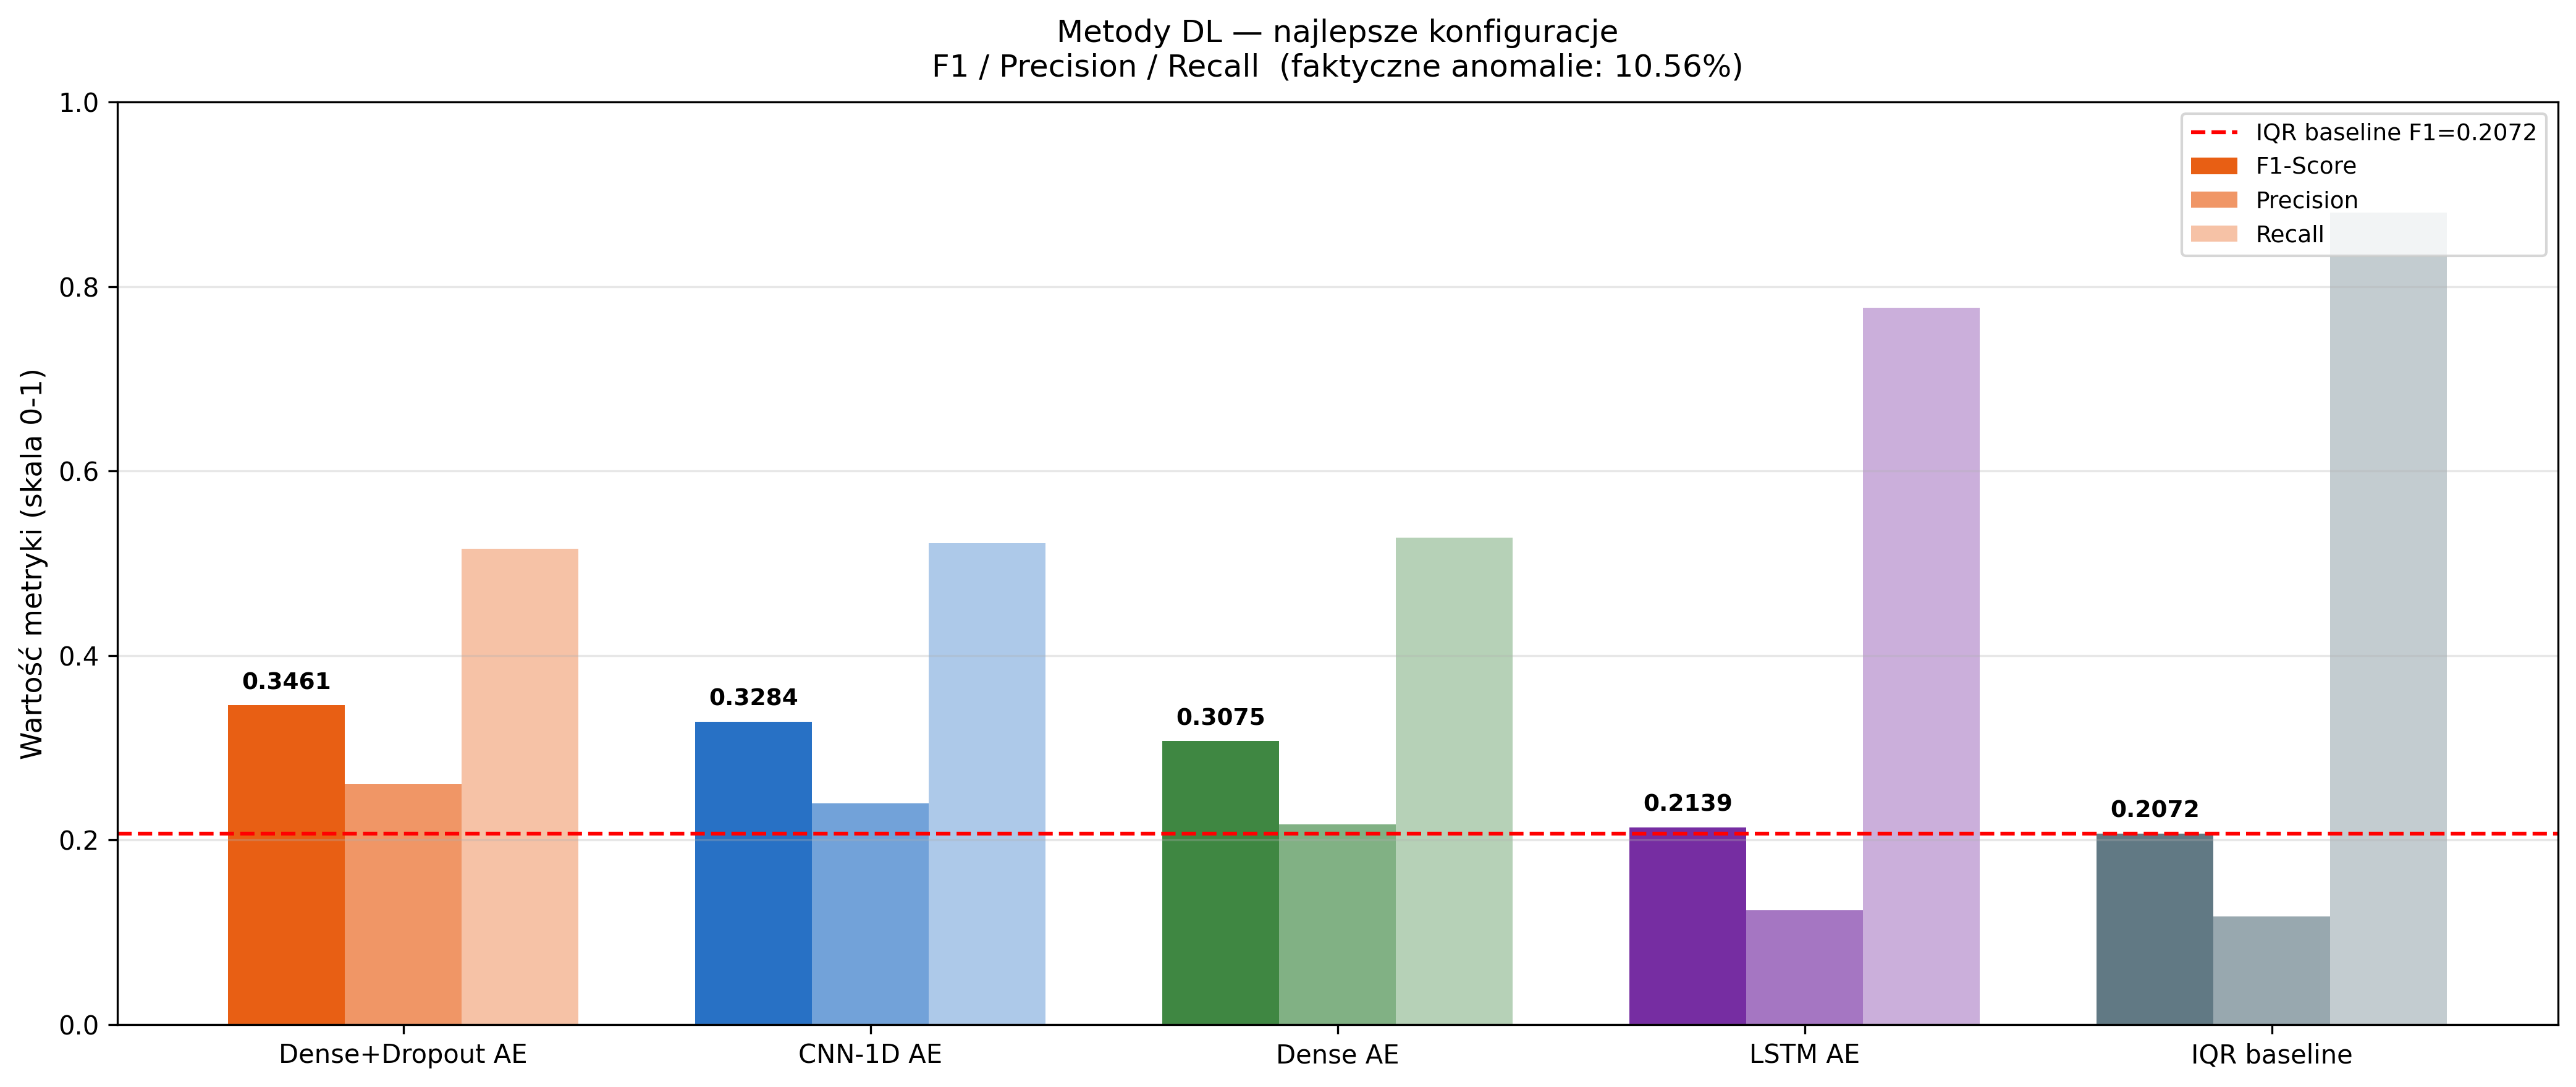
\includegraphics[width=0.9\textwidth]{fig_04b_comparison.png}
		\caption{Zestawienie skuteczności architektur opartych na głębokich sieciach neuronowych.}
		\label{fig:04b-comparison}
	\end{figure}
	
	\begin{figure}%[H]
		\centering
		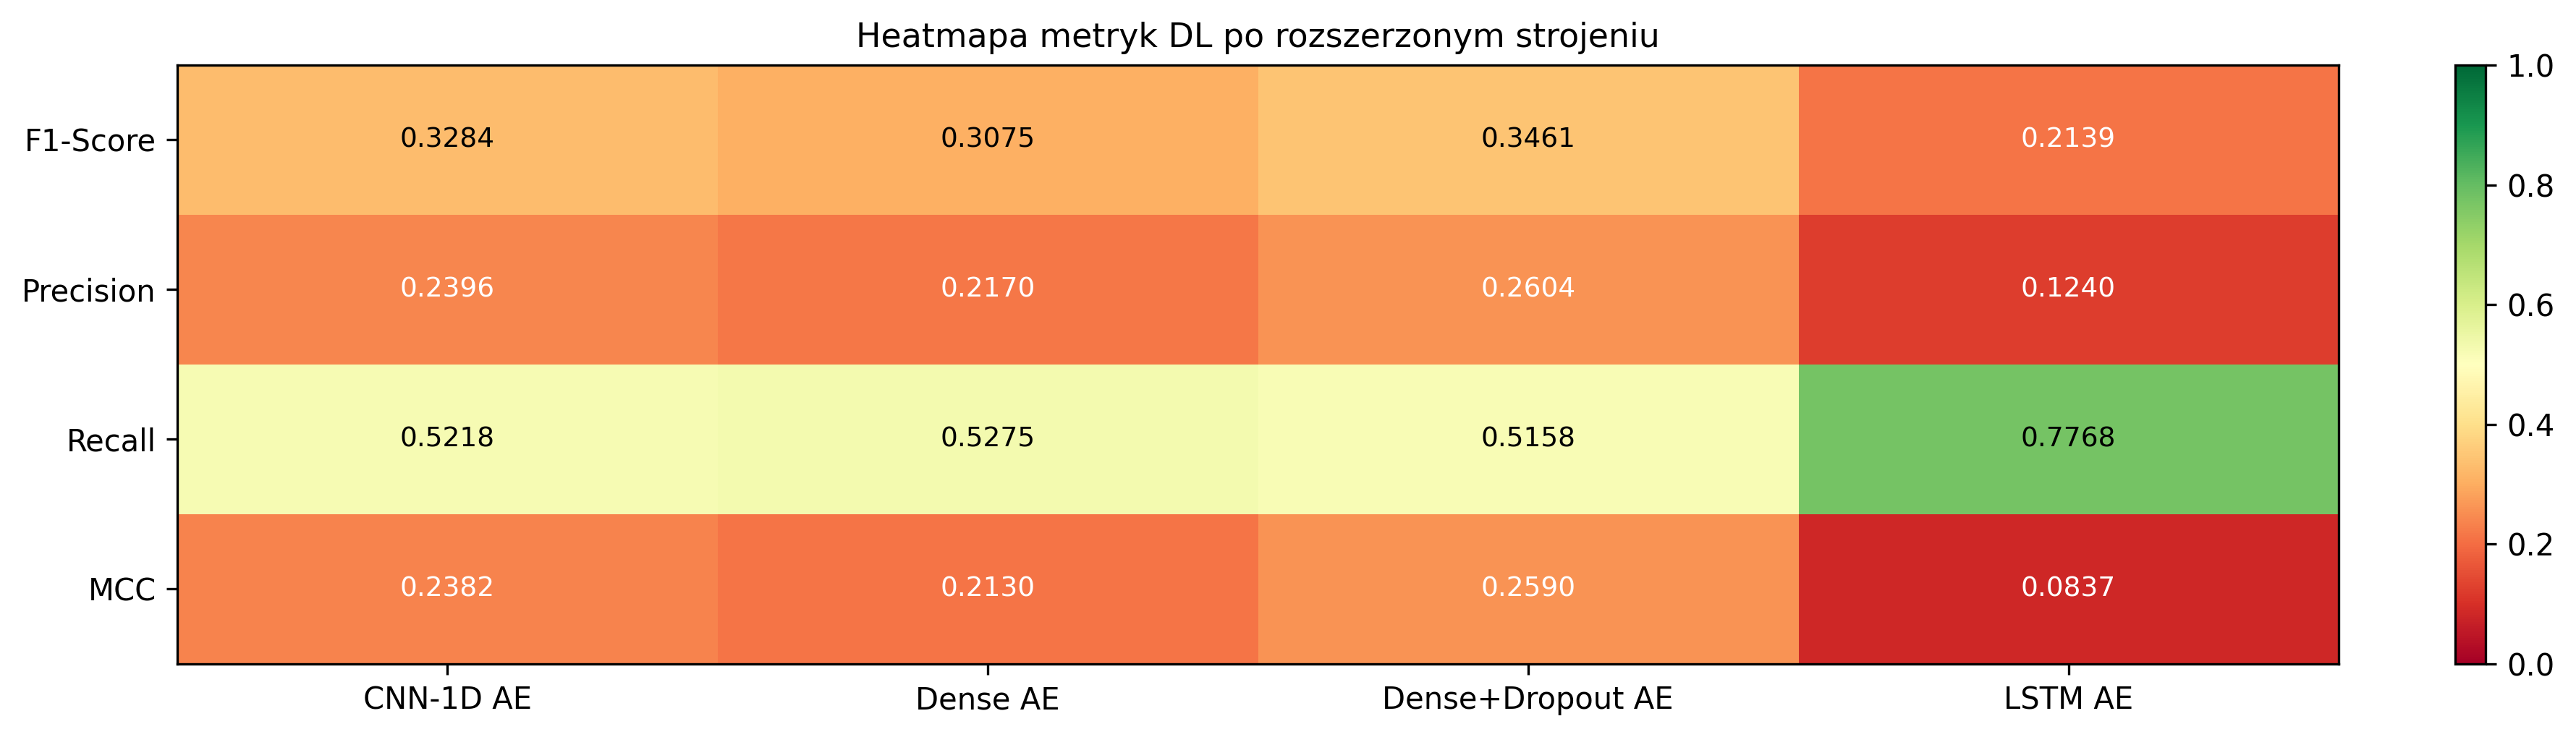
\includegraphics[width=0.9\textwidth]{fig_04b_heatmap.png}
		\caption{ Porównanie parametrów ewaluacyjnych architektur DL.}
		\label{fig:04b-heatmap}
	\end{figure}
	
	Rysunki \ref{fig:04b-comparison} i \ref{fig:04b-heatmap} prezentują zbiorcze porównanie metod głębokiego uczenia pod kątem wykrywania anomalii. Trzy z czterech metod  wyraźnie polepszyły wyniki uzyskane przez punkt odniesienia i metody uczenia maszynowego. Najlepszą okazała się być architektura gęstej sieci neuronowej z zastosowaniem mechanizmu Dropout (F1\,=\,0{,}3461). Wyniki pokazują też, że najbardziej zaawansowane metody przy ograniczonych zasobach platformy badawczej nie dają lepszych wyników, w porównaniu z prostszymi metodami, ale z odpowiednią regulacją. O skuteczności metody decyduje nie głębokość architektury, a zdolność do nauki na całym zbiorze treningowym bez większych ograniczeń pamięciowych, co przyczyniło się do klęski metody LSTM. 
	
	
	\section{Porównanie metod}
	
	\begin{tabular}{llccc}
		\toprule
		\label{tab:zbiorcza-wyniki}
		\textbf{Model} & \textbf{Typ} & \textbf{Precision} 
		& \textbf{Recall} & \textbf{F1-Score} \\
		\midrule
		IQR (baseline)    & Stat. & 0{,}1304 & 0{,}7279 & 0{,}2211 \\
		Z-Score           & Stat. & 0{,}1222 & 0{,}6446 & 0{,}2055 \\
		Z-Score Mod       & Stat. & 0{,}1311 & 0{,}7018 & 0{,}2210 \\
		CUSUM raw         & Stat. & 0{,}1108 & 0{,}9449 & 0{,}1984 \\
		EWMA              & Stat. & 0{,}1089 & 0{,}9999 & 0{,}1964 \\
		\midrule
		Isolation Forest  & ML   & 0{,}1880 & 0{,}4300 & 0{,}2616 \\
		LOF               & ML   & 0{,}2323 & 0{,}2874 & 0{,}2569 \\
		One-Class SVM     & ML   & 0{,}1282 & 0{,}8421 & 0{,}2225 \\
		K-Means           & ML   & 0{,}1674 & 0{,}1155 & 0{,}1367 \\
		\midrule
		Dense AE          & DL   & 0{,}2170 & 0{,}5275 & 0{,}3075 \\
		Dense+Dropout AE  & DL   & 0{,}2604 & 0{,}5158 & \textbf{0{,}3461} \\
		CNN-1D AE         & DL   & 0{,}2396 & 0{,}5218 & 0{,}3284 \\
		LSTM AE           & DL   & 0{,}1240 & 0{,}7768 & 0{,}2139 \\
		\bottomrule
	\end{tabular}
	
	Tabela \ref{tab:zbiorcza-wyniki} zestawia ze sobą wyniki wszystkich metod testowanych w ramach badań pod kątem miar wykrywania anomalii. Metody statystyczne skupiły się w wąskim przedziale F1 \,=\,0{,}196--0{,}221, nie przekraczając punktu odniesienia wyznaczonego, przez metodę IQR. Metody uczenia maszynowego radziły sobie lepiej (F1\,=\,0{,}259--0{,}260 dla IF i LOF), choć K-Means wyróżnia się na tle grupy, poprzez odstawanie wynikami. Metody głębokiego uczenia (z wyłączeniem LSTM) posiadają F1\,=\,0{,}308--0{,}346, wyraźnie wychodząc przed szereg względem pozostałych klas.
	
	Warto spojrzeć też na pozostałe miary, czyli precyzję i czułość. LSTM i całość metod statystycznych posiadają wysoką czułość, ale kosztem niskiej precyzji, co oznacza małą wrażliwość na szczegóły i częste alarmowanie, co przekłada się na niższe F1. Metoda gęstej sieci z dropoutem posiadała najlepszą precyzję (0{,}2604), co w połączeniu ze średnim poziomem czułości (0{,}5158) okazała się najlepszą metodą w całym eksperymencie pod względem wyników. 
	
	
	\section{Testy statystyczne}
	Zanim wyniki testów zostaną uznane za zasadne, trzeba zapewnić, że nie są one zależne od konkretnego podziału zbioru danych na treningowy i testowy, a także od losowości pewnych algorytmów. W celu oceny stabilności i istotności statystycznej różnic, postanowiono rozszerzyć procedurę badań o dodatkowe analizy, którymi są przedziały ufności i test różnicy F1 parami z dodatkową korektą wielokrotnych porównań. 
	
	\subsection{Metodologia}
	Z powodu brakujących wektorów predykcji w badaniach wszystkich metod, zastosowano \textbf{bootstrap parametryczny oparty na zapisanych macierzach pomyłek}. Każda metoda posiadała swoje wartości macierzy błędów, czyli TP, FP, FN i TN, które wyznaczają rozkład multinomialny wyników klasyfikacji. Dla każdej iteracji wykonywanego testu, losowane były nowe wartości macierzy pomyłek z tego rozkładu. Następnie dla niego wyliczano miarę F1-Score i gromadzono rozkład empiryczny. Dla tych eksperymentów ustalono ilość iteracji testu na $B = 5000$, a poziom ufności $\alpha$ na wartość 0{,}95.
	
	Porównania par metod wykrywania anomalii przeprowadzono  \textbf{bootstrapowym testem różnicy F1}. Działa on poprzez wyznaczenie empirycznego rozkład różnicy $\Delta\text{F1} = \text{F1}_B - \text{F1}_A$, a~p-wartość obliczono jako procent iteracji, dla których $\Delta\text{F1} \leq 0$ (zakładając, że B > lepsze). Jest to niesparowany test oparty na agregatach, co umożliwia porównanie metod ewaluowanych na różnych rozmiarach zbiorów, co jest podyktowane ograniczeniem próbek treningowych dla metod uczenia maszynowego LOF i One-Class SVM, a grupami DL i statystycznymi. Wszystkie wartości z 91 porównań par zostały skorygowane jeszcze \textbf{metodą Holma}, dla $\alpha$ = 0{,}05. Jest to procedura krokowa, która ma za zadanie kontrolę współczynnika błędu rodzinnego. Należy wspomnieć, że przy kilkumilionowej próbce testowej dla metod statystycznych i większej dla głębokiego uczenia, przedziały ufności są dość wąskie. Powoduje to niska wariancja F1 dla dużych próbek, co jest właściwością wyników z prawa wielkich liczb.   
	Przedziały ufności
	
	\subsection{Przedziały ufności}
	
	Tabela \ref{tab:bootstrap_ci} prezentuje wyniki najlepszej konfiguracji każdej z testowanych metod w ramach badań z przedziałami ufności dla głównych miar ewaluacji, czyli F1, precyzji i czułości. 
	Analiza potwierdziła stabilność większości wyników. Dla poszczególnych metod przedziały się nie nakładają w grupie, gdyż każda z nich zajmuje swoją część, co znaczy, że różnice w F1 nie są wynikiem losowości. Jest tylko jeden wyjątek, którym jest para IQR i zmodyfikowanej metody Z-Score, gdzie przedziały są prawie identyczne, co zostało udowodnione poprzez test różnicy parami.
	
	\begin{table}[ht]
		\centering
		\caption{Najlepsze konfiguracje metod z 95\% przedzialami ufnosci (bootstrap parametryczny, $B=5000$).}
		\label{tab:bootstrap_ci}
		\small
		\begin{tabular}{llccc}
			\toprule
			Grupa & Metoda & F1 [95\% CI] & Precision [95\% CI] & Recall [95\% CI] \\
			\midrule
			Deep Learning & Dense+Dropout AE & 0.3461 [0.3454, 0.3467] & 0.2604 [0.2598, 0.2609] & 0.5158 [0.5149, 0.5167] \\
			& CNN-1D AE & 0.3284 [0.3278, 0.3290] & 0.2396 [0.2390, 0.2401] & 0.5218 [0.5210, 0.5227] \\
			& Dense AE & 0.3075 [0.3070, 0.3081] & 0.2170 [0.2166, 0.2175] & 0.5275 [0.5266, 0.5284] \\
			& LSTM AE & 0.2139 [0.2136, 0.2143] & 0.1240 [0.1238, 0.1243] & 0.7768 [0.7761, 0.7775] \\
			\midrule
			ML & Isolation Forest & 0.2616 [0.2605, 0.2628] & 0.1880 [0.1870, 0.1889] & 0.4300 [0.4282, 0.4317] \\
			& LOF & 0.2569 [0.2556, 0.2583] & 0.2323 [0.2309, 0.2336] & 0.2874 [0.2858, 0.2890] \\
			& One-Class SVM & 0.2225 [0.2218, 0.2232] & 0.1282 [0.1278, 0.1287] & 0.8421 [0.8408, 0.8433] \\
			& K-Means & 0.1367 [0.1354, 0.1380] & 0.1674 [0.1657, 0.1689] & 0.1155 [0.1144, 0.1166] \\
			\midrule
			Statystyczne & IQR & 0.2211 [0.2203, 0.2219] & 0.1304 [0.1298, 0.1309] & 0.7279 [0.7262, 0.7295] \\
			& Z-Score Mod & 0.2210 [0.2202, 0.2217] & 0.1311 [0.1306, 0.1316] & 0.7018 [0.7002, 0.7034] \\
			& Z-Score & 0.2055 [0.2047, 0.2062] & 0.1222 [0.1217, 0.1227] & 0.6446 [0.6429, 0.6463] \\
			& CUSUM raw & 0.1984 [0.1977, 0.1990] & 0.1108 [0.1104, 0.1112] & 0.9449 [0.9441, 0.9457] \\
			& EWMA & 0.1964 [0.1958, 0.1970] & 0.1089 [0.1085, 0.1093] & 0.9999 [0.9999, 0.9999] \\
			& EWMA raw & 0.1911 [0.1905, 0.1917] & 0.1062 [0.1058, 0.1066] & 0.9518 [0.9511, 0.9526] \\
			\bottomrule
		\end{tabular}
	\end{table}
	
	\subsection{Testy różnicy}
	
	W ramach testów sprawdzono 91 par metod, z których 90 miało istotność statystyczną po korekcie Holma ($p < 0{,}05$). Jedyną konfiguracją, która okazała się nieistotna pod względem statystycznym, była para IQR – Z-Score Mod, gdzie ($\Delta\text{F1} = -0{,}0001$, z kolei $p_\text{Holm} = 0{,}788$). W momencie, w którym cechy lokalne wyznaczone, przez mechanizm okna kroczącego są już wycentrowane, zastosowanie MAD nie daje dodatkowej korzyści. Porównania metod z różnych klas, czyli statystyczne i ML, ML i DL itd., są istotne pod względem statystycznym, co daje potwierdzenie, że prymat metod głębokiego uczenia, z wyłączeniem LSTM, nad resztą nie jest wynikiem przypadku. Wszystkie pary wewnątrz grupy metod głębokiego uczenia są istotne, wliczając parę najlepszych metod, czyli Dense + Dropout i CNN-1D, w których ($\Delta\text{F1} = 0{,}0177$, $p_\text{Holm} = 0{,}018$). Różnica między nimi jest realna statystycznie, pomimo tego, że wartość bezwzględna jest względnie niska. Wybrane kluczowe porównania zostały ukazane w tabeli \ref{tab:pary_kluczowe}. 
	
	\begin{table}%[H]
		\centering
		\caption{Wybrane kluczowe porównania parami -- bootstrapowy
			test różnicy F1 z~korektą Holma ($\alpha=0{,}05$).}
		\label{tab:pary_kluczowe}
		\small
		\begin{tabular}{llcccc}
			\toprule
			\textbf{Metoda A} & \textbf{Metoda B}
			& $\Delta$\textbf{F1}
			& \textbf{95\% CI różnicy}
			& $p_\text{Holm}$
			& \textbf{Istotna} \\
			\midrule
			IQR (baseline)   & Dense+Dropout AE & $+0{,}1250$ & --- & $<0{,}001$ & Tak \\
			IQR (baseline)   & Isolation Forest & $+0{,}0405$ & --- & $<0{,}001$ & Tak \\
			Isolation Forest & Dense+Dropout AE & $+0{,}0845$ & --- & $<0{,}001$ & Tak \\
			Dense+Dropout AE & CNN-1D AE        & $-0{,}0177$ & --- & $0{,}018$  & Tak \\
			Dense+Dropout AE & LSTM AE          & $-0{,}1322$ & --- & $<0{,}001$ & Tak \\
			IQR              & Z-Score Mod      & $-0{,}0001$ & --- & $0{,}788$  & \textbf{Nie} \\
			\bottomrule
		\end{tabular}
	\end{table}
	
	\subsection{Obserwacje}
	
	Testy statystyczne wysunęły poniższe wnioski:
	
	\begin{enumerate}
		\item \textbf{Istotność hierarchiczna grup.} Porównania pomiędzy grupami metod po korekcie Holma są istotne. Dzięki temu można stwierdzić, że poprawa wyników po przechodzeniu do bardziej zaawansowanych metod nie jest dziełem przypadku.
		\item \textbf{Prymat metody Dense + Dropout} nad pozostałymi, w tym nad CNN-1D ($p = 0{,}018$).
		\item \textbf{Jedna metoda statystycznie nierozróżnialna}. IQR i Z-Score Mod ($p = 0{,}788$) jest jedyną parą metod nieistotną statystycznie. Modyfikacja już wcześniej odpornych estymatorów nie ma pozytywnego efektu na tym zbiorze danych.
		\item \textbf{Dość niskie CI}, w których szerokość wynosi $\approx 0{,}001$, jest właściwością przy $n > 10^6$ próbek, a nie artefaktem, co potwierdza, że wyniki są powtarzalne i stabilne.
	\end{enumerate}
	
	\newpage	
	\section{Koszt obliczeniowy metod}
	
	Wynik trzech głównych miar to tylko cześć łącznej ewaluacji metod wykrywania anomalii. Poza skutecznością detekcji istotną rolę ma koszt obliczeniowy, który przekłada się na czas działania algorytmu i zużycie pamięci. Nie zawsze jakość wyników danej metody idzie ramię w ramię z łatwością wdrożeniową. W ramach tej ewaluacji mierzono kilka wartości. Czas danej metody badany był jako mediana czasu dla wszystkich konfiguracji z dodaniem czasu minimalnego. Jako koszt pamięci uznano moment, w którym osiągnięto punkt szczytowy. F1-Score jest używany jako odniesienie do metryki. Wszystkie te wartości mają za cel postawione znalezienie odpowiedniego kompromisu jakości metody i kosztu obliczeniowego. 
	\begin{figure}
		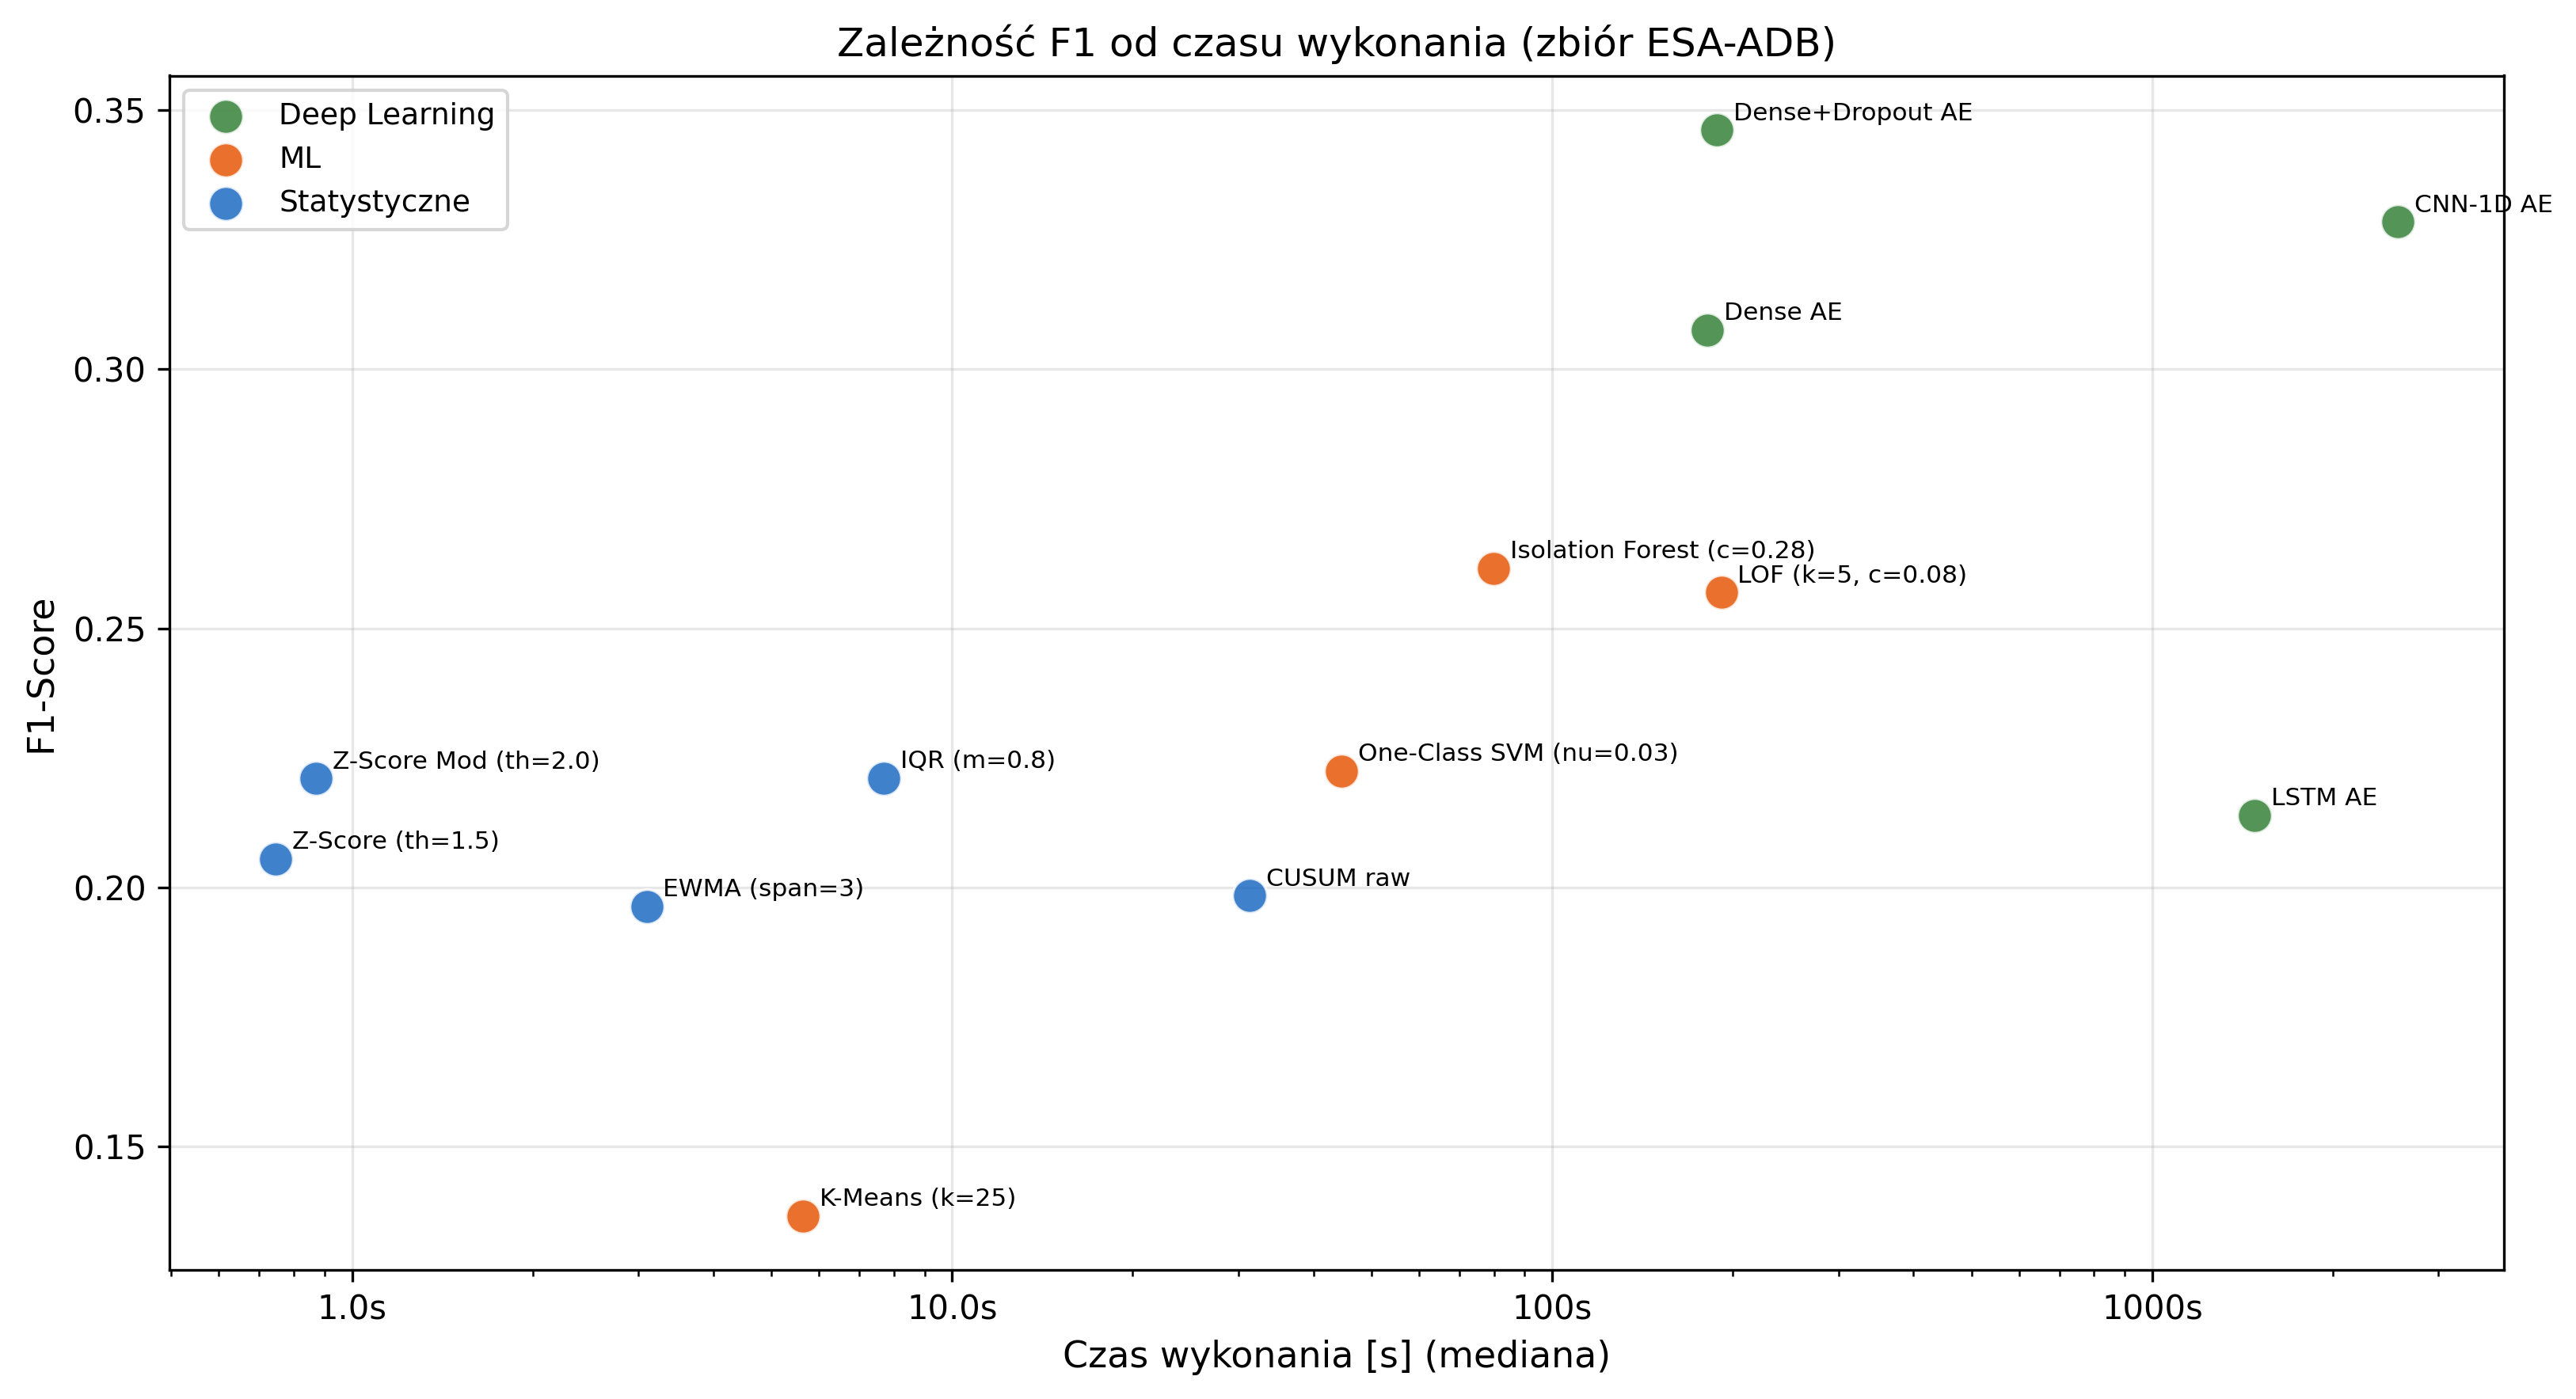
\includegraphics[width=\textwidth]{fig_05_f1_vs_time.png}
		\caption{Zależność F1 od czasu wykonywania eksperymentu}
		\label{fig:05-time-f1}
	\end{figure}	
	Rysunek \ref{fig:05-time-f1} zestawia wyniki F1-Score wszystkich metod z medianą czasów wykonania danej metody. Metody statystyczne okazały się być najszybszymi z badanych z wynikiem raptem kilku sekund na ewaluację. Wśród nich metoda IQR, uznawana za punkt odniesienia do pozostałych, daje dobry kompromis w całej grupie. Dała najlepszy wynik i tylko metoda CUSUM wykonywała się dłużej. Natomiast metoda zmodyfikowanego Z-Score, która okazała się nieistotna statystycznie, ma jedną zaletę. Wykonując się szybciej, daje prawie identyczny F1-Score. Metody uczenia maszynowego, z racji większej złożoności, wykonywała się w większym czasie, ale dając lepsze wyniki F1. Metoda Isolation Forest wyróżnia się najlepszymi wynikami miar i w miarę lepszym czasem niż druga najlepsza, czyli LOF. Wykonanie tego algorytmu trwało poniżej 80 sekund, co nie jest przesadnie dużym wynikiem, zakładając rozmiar zbioru testowego. LOF dał porównywalne wyniki w czasie 191{,}2~s, czyniąc go gorszym w obu aspektach porównania. Algorytm K-Means liczył bardzo szybko, bo w ciągu pojedynczych sekund, ale wyniki miał zdecydowanie najgorsze ze wszystkich badanych metod. Metody głębokiego uczenia okazały się jeszcze lepsze całościowo w porównaniu do innych grup, natomiast potrzebowały zdecydowanie najwięcej czasu. W najbardziej wymagającym przypadkach, czyli LSTM opartym na architekturze sieci rekurencyjnej i  CNN, działających na sieci konwolucyjnej, czasy  przekraczały próg 1000  sekund. Dla LSTM mediana wyniosła 1479{,}5 sekundy, czyli prawie 25 minut. Metoda CNN-1D, liczyła 2563 sekundy, co oznacza ponad 40 minut. Jest to spowodowane trenowaniem sieci konwolucyjnej przez 100 epok. Dla porównania metoda Dense + Dropout trenowała przez 12 epok.  Zdecydowanie lepiej pod względem czasu wypadają autoenkodery oparte na sieci gęstej, które wykonywały swoje testy w nieco ponad 3 minuty. 
	
	\begin{figure}
		\centering
		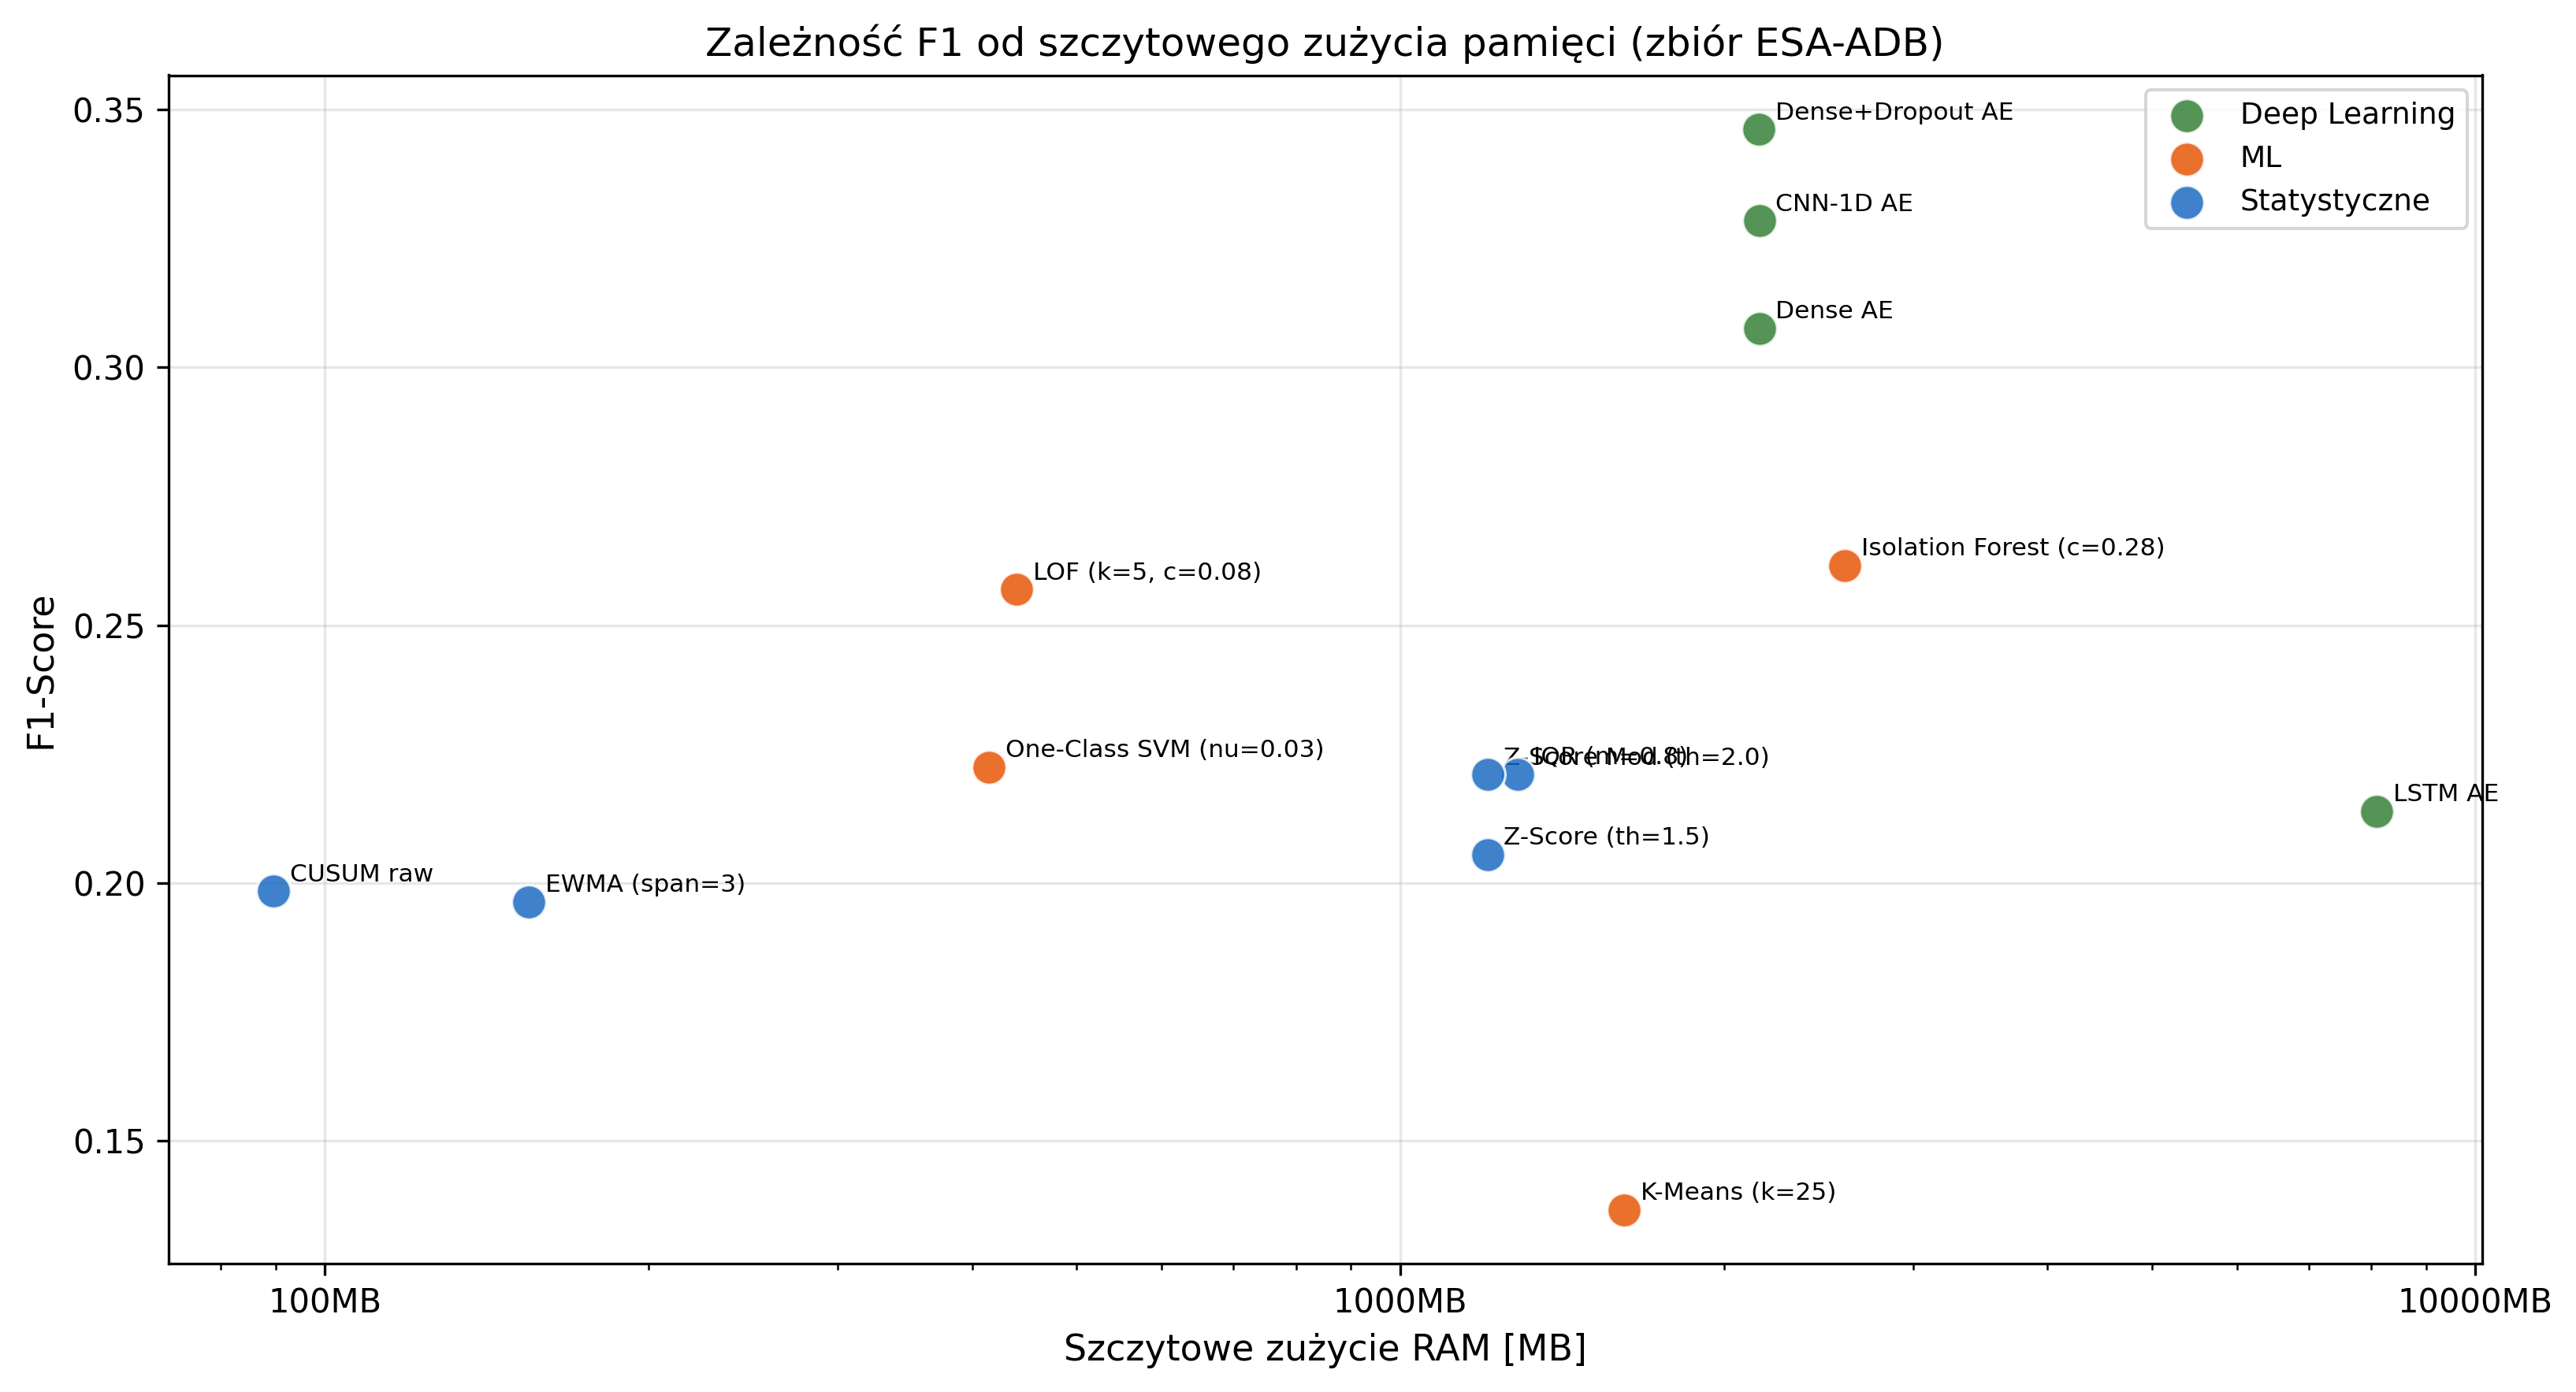
\includegraphics[width=\textwidth]{fig_05_memory_vs_f1.png}
		\caption{Zależność F1 od wykorzystanej pamięci przez metodę}
		\label{fig:05-memory-f1}
	\end{figure}
	
	Koszt zużycia pamięci w odniesieniu do uzyskanego wyniku F1-Score prezentuje rysunek \ref{fig:05-memory-f1}. Obserwacje nieznacznie różnią się w porównaniu z czasem wykonania. Niezaprzeczalnie najkosztowniejszą metodą pod kątem szczytowego wykorzystania pamięci okazał się autoenkoder rekurencyjny, który zużył ponad 8000 MB w szczytowym momencie. Pozostałe metody z grupy głębokiego uczenia osiągnęły bardzo zbliżone wyniki w okolicach 2150 MB, co okazało się mniejszą liczbą niż algorytm Isolation Forest, który potrzebował prawie 2600 MB. Algorytm LOF, który potrzebował więcej czasu do wykonania, osiągnął koszt na poziomie 440 MB, który okazał się niższy, niż  metod statystycznych . To czyni ewaluację algorytmów nieoczywistą, zależną od tego, co badacz uznaje za najważniejsze: wynik miar, czy koszt czasu i pamięci. 
	
	Wnioski z tego rodzaju badań są następujące:
	\begin{enumerate}
		\item Dense  + Dropout AE posiada najlepsze wyniki metryk, a koszty obliczeniowe nie są przesadzone.
		\item Isolation Forest zyskuje, gdy zależy nam na czasie wykonania. 
		\item Meotdy Z-Score, czy IQR posiadają najniższe czasy wykonania, wyniki osiągają w ciągu kilku sekund. 
		\item Autoenkoder rekurencyjny, zgodnie ze swoją naturą, okazał się najmniej opłacalny, wyraźnie górując nad innymi pod względem kosztów pamięci i znajdując się wśród najdłuższych metod. 
	\end{enumerate}
	
	% TODO
	
	\chapter{Podsumowanie}
	
	Celem pracy było opracowanie, implementacja, oraz badanie oceny skuteczności wybranych metod z trzech różnych paradygmatów analitycznych, jakimi były metody statystyczne, uczenia maszynowego i głębokiego uczenia w zakresie problemu detekcji anomalii w szeregu czasowym, który został zrealizowany w ramach serii eksperymentów na ogromnym zbiorze danych ESA-ADB. Dzięki wdrożeniu autorskiego rurociągu badawczego, na który składały się inżynieria cech przy użyciu techniki okna kroczącego, optymalizacji parametrów każdej metody badawczej i analiza istotności statystycznej i kosztu obliczeniowego, które dodają dodatkowy wymiar oceny poszczególnej metody
	Wyniki uzyskane w trakcie badań dowodzą znaczenia doboru klasy metod na zdolności modelu do wykrywania złożonych sekwencyjnych anomalii. Proste metody statystyczne  (np. IQR, Z-Score), choć skuteczne w detekcji pojedynczych skoków sygnału, co poparte jest wysoką czułością wszystkich metod, gdzie niektóre konfiguracje przekraczały wartość $0{,}94$, posiadają braki w wykrywaniu złożonych wielowymiarowych generalizacji. Niska wartość precyzji w tych metodach, oznacza generowanie wielkiej ilości fałszywych alarmów, co nie jest pożądane w rzeczywistych systemach. Wartość miary $F_1$, która jest średnią harmoniczną miar precyzji i czułości dla punktu odniesienia, jakim była metoda IQR, wyniosła zaledwie 0{,}2211, co okazało się progiem nie do przekroczenia dla progowania jednowymiarowego. Metody oparte na uczeniu maszynowym (ML) osiągnęły poprawę w detekcji nieliniowych zależności. W tej grupie najlepszy okazał się algorytm Isolation Forest osiągając $F_1$ na poziomie 0{,}2616. Losowy podział przestrzeni, na którym opiera się ta metoda, okazał się skuteczniejszym podejściem, a niżeli analiza lokalnej gęstości badanego punktu (na której opiera się algorytm LOF). Wynik metody K-Means okazał się porażką, osiągając najniższą wartość $F_1$ na poziomie 0{,}1367, na podstawie czego nasuwa się następujący wniosek: metody oparte na odległości euklidesowej od centroidu nie radzą sobie z zaszumionymi szeregami czasowymi, gdzie anomalią jest głównie zmiana wariancji i trendu sygnału. Modele głębokiego uczenia, oparte na koncepcji autoenkodera okazały się najlepsze w zestawieniu, dzięki wielowymiarowej rekonstrukcji sygnału. W całym badaniu najlepszą metodą okazała się metoda gęstej sieci neuronowej z mechanizmem Dropout, osiągając $F_1$ równe0{,}3461. Kluczowym dla tego wyniku było zastosowanie mechanizmu Dropout, który losowo wyłącza poszczególne neurony, co zmusza sieć do nauki bardziej uniwersalnych i rozproszonych sygnałów, co zapobiegło przuczeniu sieci. Architektura konwolucyjna również osiągnęła dobry wynik na tle pozostałych, gdyż miara $F_1$ wyniosła 0{,}3284, co czyni lokalne filtry przesuwające się po sekwencji czasowej użytecznymi w zagadnieniu detekcji anomalii. Trzeba natomiast zwrócić uwagę, na słaby wynik architektury LSTM, która osiągnęła $F_1$ na poziomie 0{,}2139. Nie jest to zasługa samej metody, a raczej ograniczeń w platformie badawczej, które narzuciły małą próbkę badawczą, z powodu ogromnych kosztów pamięciowych, które doprowadziły do przeuczenia sieci i słabej generalizacji na zbiorze testowym. 
	
	Same wartości miar ewaluacji nie daja pełnego obrazu skuteczności metod i użyteczności w scenariuszach rzeczywistego nadzoru danych w środowiskach badawczych. Przeprowadzono analizę kosztów obliczeniowych, które uzupełniają dane metody ewaluacji o zużycie czasu i pamięci na wykonanie modelu. Badania te ukazały znaczny rozkład zużytych środków między metodami. Metody statystyczne dokonały ewaluacji na zbiorze testowym w ciągu pojedynczych sekund bez większego obciążenia zasobów pamięci. Architektury bardziej złożone, takie jak metody ML i autoenkodery potrzebowały więcej zasobów do przeprowadzenia oceny skuteczności modelu. Największą ilość czasu i pamięci do ewaluacji potrzebowała architektura rekurencyjnej sieci neuronowej, w postaci metody LSTM.   Pomimo tego, że nie zajęła największego czasu, gdyż tylko architektura CNN potrzebowała więcej czasu, natomiast są to jedyne metody, których mediana czasu potrzebnego przekroczyła próg 1000 sekund. Natomiast wynik zużycia pamięci jest jeszcze mniej korzystny dla metody LSTM. W szczytowym momencie model zużył ponad $8000$ MB pamięci RAM. Po raz kolejny architektura gęstej sieci neuronowej z zastosowanym mechanizmem Dropout dała najlepszy kompromis, potrzebując nieco ponad 3 minut i zużywając $2150$ MB pamięci. To czyni tą metodę najbardziej perspektywiczną w potencjalnym wdrożeniu w systemach kontroli i monitorowania danych. 
	
	Zastsowanie testów statystycznych pozwoliło na większa uwiarygodnienie wyników. Testy bootstrapowe z korektą Holma udowodniły, że hierarchia metod pod kątem wyników nie jest wynikiem losowości i przypadku. Wykazano istotną różnicę ($p = 0.018$) między dwoma najlepszymi metodami, jakimi były architektura gęsta z  Dropoutem i sieć konwolucyjna. W ramach testów uznano tylko jedna parę danych za nieistotną statystycznie. Okazały się nimi para metody IQR i zmodykowany Z-Score, który osiągnął ($p = 0.788$). Jest to dowód matematyczny na to, że aplikowanie miar odpornych na zmianę charatkeru sygnału w metodach statystycznych, takich jak MAD, mija się z celem, w przypadku gdy dane badane zostały już podane wstępnej inżynierii cech nakładającą cechy lokalne poprzez okno kroczące. 
	Pomimo realizacji założonych celów, badania przeprowadzone mają swoje ograniczenia. Przede wszystkim mowa tu o ograniczeniach sprzętowych, które wywołały przymus redukcji rozmiaru próbki badawczej dla niektórych metod, głównie głębokiego uczenia i One-Class SVM. Szczególnie w przypadku metody LSTM użycie pełnego zbioru, może mieć pozytywny wpływ na wartość miar mierzonych w ewaluacji modeli. Ponadto, w samym badaniu użyto tylko 6 kanałów zbioru danych, który posiada ich znacznie więcej, a same kanały są dość niezbilansowane, co może mieć negatywny wpływ na skuteczność metod progowych. Biorąc te obserwacje pod uwagę w ramach dalszych prac powinno się skupić na implementacji badań na bardziej adekwatnej platformie sprzętowej niż laptop do codziennej pracy. Wtedy można ocenić prawdziwą skuteczność badanych metod, a nie w przypadku skrajnego scenariuszu. Dodatkowo zauważono ograniczenia niektórych metod z racji swojej natury. W literaturze naukowej często w ramach detekcji anomalii stosuje się połączenie kilku metod, tworząc algorytmy hybrydowe \cite{ rana2022hybrid}. Kolejnym obszarem , który można poruszyć w ramach rozwoju jest zastosowanie algorytmów metaheurystycznych do optymalizacji parametrów strojonych w każdej metodzie. W wykonanych badaniach testowane parametry zostały testowane przez kosztowne przeszukiwanie siatki (Grid Search) co tworzyło dużą liczbę testowanych konfiguracji, co miało przełożenie na czas badania, który sięgał kilkanaście godzin nieprzerwanej pracy. Skupienie się na tych kierunkach rozwoju stanowi naturalną ewolucję systemu monitorowania, która za zadanie będzie miała zwiększenie bezawaryjności modeli, które będą służyć rozwojowi technologicznemu i poznawczemu.

	
	\cleardoublepage
	\phantomsection
	%\bibliographystyle{plplain}  % bibtex
	%\bibliography{biblio} % bibtex
	\addcontentsline{toc}{chapter}{Bibliografia}
	\printbibliography           % biblatex
	
	\begin{appendices}
		
		% TODO
		\chapter{Dokumentacja techniczna}
		
		
		% TODO
		\chapter{Spis skrótów i symboli}
		
		\begin{itemize}
			\item[DNA] kwas deoksyrybonukleinowy (ang. \english{deoxyribonucleic acid})
			\item[MVC] model -- widok -- kontroler (ang. \english{model--view--controller}) 
			\item[$N$] liczebność zbioru danych
			\item[$\mu$] stopnień przyleżności do zbioru
			\item[$\mathbb{E}$] zbiór krawędzi grafu
			\item[$\mathcal{L}$] transformata Laplace'a 
		\end{itemize}
		
		% TODO
		\chapter{Lista dodatkowych plików, uzupełniających tekst pracy (jeżeli dotyczy)} 
		
		W systemie do pracy dołączono dodatkowe pliki zawierające:
		\begin{itemize}
			\item źródła programu,
			\item zbiory danych użyte w~eksperymentach,
			\item film pokazujący działanie opracowanego oprogramowania lub zaprojektowanego i wykonanego urządzenia,
			\item itp.
		\end{itemize}
		
		
		\listoffigures
		\addcontentsline{toc}{chapter}{Spis rysunków}
		\listoftables
		\addcontentsline{toc}{chapter}{Spis tabel}
		
	\end{appendices}
	
	\end{document}
	